% !Mode:: "TeX:UTF-8"
\documentclass[master,openright,oneside]{buaathesis}
\usepackage{amssymb}

%\usepackage{enumerate}
\usepackage{fancyvrb}
\usepackage[linesnumbered,boxruled,noline]{algorithm2e}
\renewcommand{\algorithmcfname}{算法}
\IncMargin{1em}
%\SetAlCapSkip{10ex}

\RequirePackage{fancyhdr}


\begin{document}

% 个人信息
% !Mode:: "TeX:UTF-8"

% 学院中英文名,中文不需要“学院”二字
% 院系英文名可参见
% http://ev.buaa.edu.cn/education/index.php?page=department
\school
{计算机}{School of Computer Science and Engineering}

% 专业中英文名,中文不需要“专业”二字
\major
{计算机系统结构}{Computer architecture}

% 论文中英文标题
\thesistitle
{一种面向通信的\\
多核分区实时调度算法研究}
{%这里是长长的长长的长长的长长的长长的长长的长长的长长的长长的副标题
}
{A Communication-Oriented Real-Time Tasks Scheduling Algorithm for Partition System on Multiprocessors}
{%English sub title, It is very very very very very very very very very very long
}

% 作者中英文名
\thesisauthor
{王锦麟}{Wang Jinlin}

% 导师中英文名
\teacher
{龙翔}{Long Xiang}

% 中图分类号,可在 http://www.ztflh.com/ 查询
\category{TP316.2}

% 学习开始时间
\thesisbegin{2010}{09}{06}

% 学习结束时间
\thesisend{2012}{12}{24}

% 毕设答辩时间
\defense{2012}{12}{24}

% 中文摘要关键字
\ckeyword{多核,实时系统,调度算法,面向通信,同步数据流} %======================

% 英文摘要关键字
\ekeyword{multiprocessor, real-time OS, scheduling algorithm, Communication-Oriented, SDF} %=============================

% 研究方向
\direction{实时系统调度算法}

% 教师职称中英文
\teacherdegree{教授}{Prof.}

% 保密等级
\mibao{}

% 论文编号,由10006+学号组成
\thesisID{10006SY1006515}

% 论文提交时间
\commit{2012}{12}{24}

% 学位授予日期
\award{\qquad}{\quad}{\quad}

% 中英封面、提名页、授权书
\maketitle

%%%%%%%%%%%%%%%%%%%%%%%%%%%%%%%%%%%%%%%%%%%%
% 摘要、目录页眉页脚

\pagestyle{fancy}
\fancyhead{}
\fancyfoot{}
\fancyfoot[C]{\zihao{5}\thepage}
%%%%%%%%%%%%%%%%%%%%%%%%%%%%%%%%%%%%%%%%%%%%%


%前文区
\frontmatter

\pagestyle{plain}
% 摘要
% !Mode:: "TeX:UTF-8"
\begin{cabstract}
本篇文档主要介绍{\bf 北航毕业设计论文\LaTeX{}模板}使用和相关软件环境的安装配置,
以及本模板所遵循的开源协议等。
\end{cabstract}
\begin{eabstract}
Here is the Abstract in English. And this is a test sentence, just for
a test to see how the buaathesis works. You can just ignore this.\par
This is another pargraph.
\end{eabstract}



%%%%%%%%%%%%%%%%%%%%%%%%%%%%%%%%%%%%
% 目录、插图目录、表格目录
\tableofcontents
\listoffigures
\listoftables

% 符号表
% !Mode:: "TeX:UTF-8"

% 改为按字母顺序排列

\begin{denotation}
  \item[COSS] 面向通信的静态调度算法 (Communication-Oriented Static Scheduling Algorithm)
  \item[DAG] 有向无环图 (Directed Acyclic Graph)
  \item[DLS] 动态层级调度 (Dynamic Level Scheduling)
  \item[DSP] 数字信号处理 (Digital Signal Processing)
  \item[GSDF] 广义同步数据流 (General Synchronous Data Flow)
  \item[ICS] 改进的 Class S 算法 (Improved Class S Algorithm)
  \item[MDLS] 修改的动态层级调度 (Modified Dynamic Level Scheduling)
  \item[SBL] 静态 B 层级 (Static B-Level)
  \item[SDF] 同步数据流 (Synchronous Data Flow)
\end{denotation}



%\begin{denotation}
%
%\item[HPC] 高性能计算 (High Performance Computing)
%\item[cluster] 集群
%\item[Itanium] 安腾
%\item[SMP] 对称多处理
%\item[API] 应用程序编程接口
%\item[PI] 聚酰亚胺
%\item[MPI] 聚酰亚胺模型化合物,N-苯基邻苯酰亚胺
%\item[PBI] 聚苯并咪唑
%\item[MPBI] 聚苯并咪唑模型化合物,N-苯基苯并咪唑
%\item[PY] 聚吡咙
%\item[PMDA-BDA] 均苯四酸二酐与联苯四胺合成的聚吡咙薄膜
%\item[$\Delta G$] 活化自由能~(Activation Free Energy)
%\item[$\chi$] 传输系数~(Transmission Coefficient)
%\item[$E$] 能量
%\item[$m$] 质量
%\item[$c$] 光速
%\item[$P$] 概率
%\item[$T$] 时间
%\item[$v$] 速度
%\end{denotation}



%%%%%%%%%%%%%%%%%%%%%%%%%%%%%%%%%%%%%%%%%%%%
% 正文页眉页脚

\pagestyle{fancy}
\fancyhead{}
\fancyfoot{}
\fancyhead[C]{\zihao{-5}\songti
    \ifodd\value{page}
        北京航空航天大学硕士学位论文\vspace{1.5mm}
    \else\leftmark
    \fi
}
\fancyfoot[C]{\zihao{5}\thepage}

\renewcommand{\headrulewidth}{0.5bp} % 页眉线宽度

\fancypagestyle{plain}{
    \pagestyle{fancy}
}

%%%%%%%%%%%%%%%%%%%%%%%%%%%%%%%%%%%%%%%%%%%%%

% 正文页码样式
\mainmatter

\normalem %去除 ulem 包的下划线

% 正文
% Introduction 国内外现状
% !Mode:: "TeX:UTF-8"
\chapter{绪论}

% \emph{TODO: 调整格式、补全引用}

\section{课题研究背景}

% -------------------------------
\subsection{多核分区系统}
在航空电子等方面,传统的联合式结构中,每个单独的计算机系统只负责某一项具体的应用功能,所有功能模块通过特定的总线接口与相关协议有机的联系起来,控制整机的正常运行。这种结构的好处是他们内在的错误具有隔离性,即一般一个功能模块的失效并不会影响其他功能的正常运行。但同时其缺点是每个功能都需要自己独占的计算机,系统中处理器的数量会随着系统功能的丰富而增加,造成整个系统在空间、电力、重量、冷却、安装、维护等方面的重复负担,增加了维护成本、限制了系统规模。

为了提高系统的集成度,增加计算机资源的利用率,人们提出了系统综合化的要求。在综合化的系统中,一个计算机系统能够为多个应用提供计算资源,从而提高系统的利用效率。但综合化系统会破坏原来硬件的天然隔离,增加错误传播的几率。为了解决这个问题,分区系统被提了出来。使用分区机制可以为运行在系统中的不同应用建立独立分区,在时间和空间两个维度提供资源,使应用之间相互隔离,保持联合式结构中的优点。

% 可以添加 综述 里关于多核发展的描述 \cite{SurveyHRT}
另一方面,随着集成电路工艺的发展遇到瓶颈,单核处理器的性能已经达到极限,单纯的通过提高主频等传统方式已经无法显著提高处理器的性能。通过多核、众核架构来更好的并行处理任务成为了新的趋势,主要处理器芯片商也纷纷推出多核产品,目前已在通用领域得到广泛应用。因此,分区系统向多核处理器平台发展也将成为不可避免的趋势。


\subsection{实时调度算法}


目前,关于多核实时系统的调度算法研究,多集中于任务的时间约束,以及提高处理器的利用率等方面\upcite{SurveyHRT}。多核的并行任务分配大部分是NP完全问题\upcite{SchOSRT},这给算法设计带来了难度。此外,多核实时调度算法针对任务间数据流通、协作而产生的偏序依赖关系的情况还缺少成熟的结论。

随着系统规模的扩大,实时任务间的关系也日趋复杂。如文章\cite{Without}中提到的情况,在构建一个关键的嵌入式控制系统时,系统中的控制循环包括传感器、控制算法和调节系统状态的传动部件等。这类系统的构建通常需要多人团队并行的分工合作,分别开发系统中的不同部分,之后再将这些部分(或者称作任务)组合成一个系统。这类集合工作经常需要人工在离线情况下对任务排序,来保证任务的执行是可预测、可确定的。但在目前成熟可靠的嵌入式操作系统中,如用于汽车工业的 OSEK\upcite{OSEK}系统、面向宇航的 RTEMS\upcite{RTEMS} 系统、以及遵循 ARINC 653 标准\upcite{ARINC653} 的航电系统(如 VxWorks 653\upcite{VxWorksRTCA})等,对带有数据依赖的任务并没有提供直接支持。这意味着任务间通信的确定性保证通常需要手工先对任务部分排序,然后再交由操作系统调度,而这个过程是冗繁的。

%再举个例子

%\section{课题来源与意义} %=========================================

\section{论文研究目标与内容}


结合以上几方面的发展趋势及多核调度算法在实际问题中所遇到的挑战,本文以多核分区系统平台的任务为模型,提出一种面向通信的调度算法,综合考虑任务的周期性时间约束和任务间由于数据通信所产生的数据依赖约束,产生满足以上约束条件的静态调度。

本文针对多核分区的实时系统,研究它的调度算法。主要研究目标包括:
\begin{enumerate}
\item	调研现有多核或实时调度算法,讨论在多核分区实时系统中,这些算法在调度包含周期性时间约束和数据通信产生的数据依赖约束的任务时所遇到的困难。包括如何解决周期任务间的依赖关系、保证实时任务的时间限制、考虑不同处理器间的通信延迟等。
\item	针对以上问题抽象出一个问题模型,在该模型上实现一种多核分区实时调度算法,在给定一个周期性任务集和他们的时间限制,并给出任务间的数据依赖关系的情况下,在目标多核分区处理器平台寻找满足以上约束条件的静态调度。在能够调度时给出考虑核间通信延迟下的一种可行调度方案。
\item	验证算法的正确性,分析算法的时空复杂度,并结合例子分析算法对通信约束的处理。
\end{enumerate}


本论文的主要研究内容有以下几个方面:
\begin{enumerate}
\item	调研多核系统现有的并行调度算法及其优势和局限性。
\item	设计调度算法,以满足对多核分区系统中有依赖关系的实时任务的有效调度。主要考虑以下问题:
  \begin{itemize}
    \item	任务的实时性要求。如周期性、时间限等。
    \item	任务的数据依赖关系约束。如任务C的执行需要任务A 和B 的输出结果时,不能使C 先于任务A 和B 执行。
    \item	核间的通信开销。当A向其他核上执行的任务B发送数据时,B要在数据到达后才能开始执行;如果A 和B 在同一处理器时不存在此延迟,或延迟可忽略。
    %\item	在给定的多核架构上充分发掘任务间的并行性,以使调度结果尽量接近最优。
  \end{itemize}
\item	从理论上证明算法对实时任务在时间上的保证。
\item	构建调度算法模拟程序,并验证调度的任务满足时间与数据约束。%并实测算法的运行效率和调度结果的优劣。
\end{enumerate}

\section{国内外研究现状}

%介绍实时任务的两方面:传统周期性约束 以及 DSP 中的数据约束
实时任务的正确性不仅要求任务运行结果在逻辑上正确,还要求任务必须在一定的时间限内运行结束。从周期性和偶发任务模型来说,实时任务包括周期性任务、偶发性任务和非周期任务等,它们的特征是任务均以时间为驱动,即任务什么时候释放、是么时间段可以执行以及任务什么时候必须执行完毕都是由时间来决定的;与此相对的,DSP 系统中的数据流程序则属于另一类的实时任务,它们以数据驱动为特征,即什么时候可以执行,哪个任务先执行,都是由任务间的数据流动来决定的。

%分两段分别介绍时间约束的实时系统,如 VxWorks 等 和 DSP 中的数据约束 各自的处理方法,如 时间系的调度为何不满足需求、SDF 系的调度为何也不满足需求
周期性和偶发任务模型是大多数传统的实时操作系统所支持的任务模型。在绝大多数发表的关于周期性和偶发任务模型的调度研究中,都假定任务间是相互独立的\upcite{SurveyHRT},即不考虑因处理器以外的资源争用造成任务阻塞。大部分多核的实时任务调度问题都是NP完全的,因此一些启发式算法被提了出来,如 Thakor, D. 和 Shah, A. 提出的D\_EDF 算法\upcite{DEDF},Zhu Xiangbin 和 Tu Shiliang 提出的基于 myopic 算法的启发式算法\upcite{Zhu2003} 等。但由于受任务模型所限,这些算法均未能考虑任务间制约关系的问题。 % 参考那篇大综述,有一章讲了争用
此外,Rajkumar 等人在\cite{Contention}中使用固定优先级的方法在多核分区系统中实现了类似单处理器调度中用于解决共享资源争用的 PCP (Priority Ceiling Protocol) 策略\upcite{SContention},一定程度上打破了周期性和偶发任务模型对于任务相互独立的限制。但这类方法用于解决多核系统中多任务互斥访问共享资源的调度问题,对于任务间数据通信所产生的先后依赖关系仍未涉及。


在数据驱动的任务模型中,由于DSP系统对大数据量吞吐率的需求,任务多采用静态调度,它的并行调度算法也较好的解决了任务间的数据传输、依赖关系等问题。设计流式程序所要面对的一个挑战是如何有效表达程序中的并行性\upcite{Challenge}。而基于计算模型 (Model-of-Computation, MoC) 的设计则成为了解决这一挑战的事实标准\upcite{MoCdefacto}。% 提出 SDF 方法
如EDWARD ASHFORD LEE 等人提出的SDF 方法\upcite{SDF1987,SDF_C} 即是一种在 DSP 中使用广泛的计算模型,它能够较好的表述任务间的数据传输、依赖关系等,并由此得到有效的静态调度表。 但由于DSP 系统是数据驱动型的,这点从本质上与时间驱动型的实时系统有所不同,DSP 中的一些调度算法(包括 SDF 相关的方法)并不能直接用来解决带有周期性时间属性的实时任务调度问题。在解决时间约束方面Margarete Sackmann 等人提出的一个考虑时间和能耗约束的快速启发式算法\upcite{FastHeu} 在解决单个任务的时间限制约束上有一定进展,但仅将时间限制作为调度的参考,没有给出理论上的严格保证,也未考虑任务的周期性约束条件等。

% 再一段介绍有些方法企图将两者结合起来,如。。。等
% 主要是那几篇解决问题比较类似的论文
也有些文章综合考虑了任务的时间约束以及任务间的偏序依赖关系。如\cite{Xujia1993}提出了这样的任务模型:有一个任务集,其中每个任务有确定的释放时间和结束时间限,每个任务又由一系列包含偏序关系和互斥关系的子任务组成。文中针对此任务模型提出了在多核平台的静态最优调度算法。虽然该模型同时考虑了任务的时间以及依赖约束,但其时间约束仅针对整个任务,对子任务没有单独的限制。此外,与本文的工作相比,\cite{Xujia1993} 中的模型也有几点不同:1)~时间约束是一次性的,未考虑周期性调度的情况;2)~未考虑任务或子任务之间通信延迟的影响。
另外,文章\cite{Without}提出并研究了关键嵌入式系统中,带有先后关系约束的周期性任务集的调度问题。文中将任务的先后关系分为两类来解决:(1)~简单先后关系:带有先后关系的任务具有相同的周期;(2)~扩展的先后关系:带有先后关系的任务可以有不同的周期。对于简单先后关系的任务,文中将任务在周期内按不同的时间偏移重新组织,保证在周期内满足任务间先后关系的约束;而对于扩展的先后关系,文中取两个周期的最小公倍数周期作为一个大周期,列举大周期内各任务多次执行之间的所有先后关系约束,将其化为相同周期的任务处理。之后,由于每个处理器上的调度仅采用固定优先级的传统周期任务实时调度算法,该策略没有能够保证任务之间先后关系的机制,因此需要单独调整各个带有先后关系的任务的周期属性,推后首次释放时间、缩减运行时间限来保证任务间的先后关系约束。这样造成的一个明显缺陷是,当任务中先后关系较多时,原本有可能调度的任务由于推后了首次释放时间和减少了时间限造成无法调度的结果。另外,本文也没有链路上的通信调度。
文章\cite{HRTSCSDF}将非环的 CSDF 图(一种类似 SDF 的计算模型)转化为周期性任务,试图在转化后仅用传统的针对相互独立任务的周期性调度算法来调度这些任务,同时还保证任务间满足 CSDF 图所述的数据依赖关系。该文的方法与\cite{Without}类似,都是希望将数据依赖关系转化为独立的周期性任务,通过调整任务的周期属性来保证任务间的先后依赖关系。由于转化为周期性任务限制了任务调度的灵活性,因此该方法并不保证对所有数据依赖都能成功转化。与之相比,本文的方法将周期性的时间约束关系转化为数据依赖关系,并与原任务间的数据依赖共同构成统一的 GSDF 图。由于上述转化过程是不损失调度灵活性的,因此该转化过程对任务的可调度性无损害。

% 中期检查

在分布式计算方面,人们对多处理器的并行调度也有较多研究,由于运算环境的复杂性,各处理器间的通信效率、时延以及整个任务集的总调度长度等方面是主要的关注点,如文章\cite{DLS} 提出的Mapping Heuristic 算法,文章\cite{Leinberger2000,Yu1991} 提出的DLS 算法等,考虑了数据通信的消息调度等问题。但同样这些算法也缺少对周期性实时性任务的支持,并不能从理论上保证任务的时间需求。


\section{论文研究成果}
%直接照搬 abstract,待修改

针对多核实时系统上的任务调度问题,本文提出一种面向通信的静态调度 (Communication-Oriented Static Scheduling, COSS) 算法。该算法能够在考虑任务间数据通信和周期任务时间限的情况下,在运行前将任务静态调度到多核处理器平台上,同时保持任务之间的通信关系和时间限制得到满足。在有效调度能够被找到的情况下,算法将会给出各个核上的调度序列,以及核之间链路上的消息调度序列。

\section{本文的组织}

本文其余部分组织如下:

第二章首先简要介绍目前主要多核实时调度算法的分类、各自的特点。其次论文讨论相关的几种多核平台的计算模型极其特点,所采用相关算法的考虑因素。第三节介绍了 DAG 调度的主要几类算法,并分析了各自的特点。第二章最后对多核分区操作系统的特点做了简要介绍。

% 直接说三四两章详细介绍算法设计,不用这么具体写每章是什么
本文三、四、五章分别详细介绍了 COSS 算法的三个步骤的具体设计及思路,给出了每个过程中所要解决的问题,以及所选取的具体方法的原因,提出了每个过程的具体算法过程,并分析了算法复杂度。

第六章根据前述算法流程的设计,介绍算法的具体实现过程,模块划分以及各模块在具体实现中遇到并解决的一些问题。

第七章从几个例子验证了调度算法对任务调度结果的正确性,并结合相同任务集在不同连接平台的调度结果分析了处理器间的连接对任务分配的影响。

% 背景知识
% 介绍基于的算法
% !Mode:: "TeX:UTF-8"

%除了通用系统的多核调度外,在各个特殊领域,如DSP系统、分布式计算、实时系统中,也对多任务多核的并行调度提出了各自的要求。DSP系统是传统的并行处理系统,其为了数据的最大吞吐率,往往要设计各处理单元间协同工作,哪些任务需要并行,哪些任务安排在相同或不同的处理器,哪些任务先执行,数据通路如何安排都需要精心设计。与之相比,分布式计算往往更注重通信方面的开销,其计算系统各运算单元间通信的不确定性,也为任务调度安排带来了新的变数。

%在 DSP 系统方面,现有算法能够较好的处理任务间的偏序关系,但 DSP 的调度算法主要是数据驱动型的,它对以强烈时间属性为特性的实时任务仍然难以满足需求。在分布式计算方面,主要关注点在于任务间通信以及总的调度长度,同样缺少调度算法对任务的时间要求给予特别的保证。


\chapter{相关技术介绍}

\section{实时调度算法背景简介}

%\subsection{实时调度算法}

%\emph{TODO: 调整格式、补全引用}

\subsection{任务模型}

一个基本的实时任务模型包括以下三类任务:
\begin{description}
  \item[周期性任务 (periodical)] 包括以下参数:\\
    周期 T;最坏执行时间 C;首次执行偏移 O;相对时间限 D。
  \item[偶发性任务 (sporadic)] 相比周期性任务,它的周期不是一定的,但有一个最小间隔时间。
  \item[非周期任务 (aperiodic)] 只释放一次的任务。
\end{description}

\subsection{任务的时间限}

周期性任务的时间限有以下三种分类:
\begin{itemize}
  \item 隐性时间限(implicit-deadline),任务的时间限与任务的释放周期相等。
  \item 限制时间限(constrained-deadline),每个任务的时间限都不长于它的释放周期。
  \item 任意时间限(arbitrary-deadline),时间限与释放周期无关。
\end{itemize}

大部分任务系统允许任务被抢占,并在以后被恢复且无额外开销。

一个周期性任务或偶发性任务的占用率(utilization)定义为
\begin{equation}
  U(t) = C/T
\end{equation}

一个由周期性任务和偶发性任务组成的任务系统的总占用率为各任务占用率之和。
以上任务模型根据实际因素会加入 非抢占约束、优先关系约束、互斥关系约束等。

%================================
\subsection{调度环境}

\subsubsection{离线调度}

离线调度也称为静态调度,所有任务的执行时间都认为是最坏情况的执行时间。由于任务的周期性,整体调度也是周期性的,其周期长度等于各任务周期的最小公倍数。因此,随着任务数量的增长,静态调度表的长度具有指数级的大小,对一些嵌入式系统的实现来说可能成为问题。

大部分实时系统内核实现基于优先级的调度器,分为静态优先级和动态优先级。静态优先级,每个任务被赋予一个固定,且与其他任务不同的优先级;动态优先级则在任务执行时多次重复计算。运行时调度选择最高优先级的任务执行。
一个调度算法是最优的,是指如果一个可行调度存在,该算法一定能找到可行调度。

在离线调度中,设计调度算法和检测调度可行性是同一个问题。调度算法根据任务的时间限得到一个可行调度序列。

\subsubsection{在线调度}

除了以上离线调度的情况外,基于优先级的在线调度需要考虑优先级反转现象(priority inversion phenomenon)。如果高优先级的任务 Tc 需要一个低优先级任务 Ta 的资源,而 Ta 根据优先级规则又被一个中等优先级的任务 Tb 抢占,造成 Tb 阻塞 Tc 执行的现象。调度非抢占式的任务,或者任务间需要通过网络传递消息时也会产生此现象。

在在线调度中,实时调度理论集中于以下两个问题:
\begin{itemize}
  \item 调度可行性分析:给定一个任务系统,和一个调度环境,确定是否存在一个调度满足所有时间限。
  \item 运行时调度问题:给定一个可行的任务系统,根据调度环境,确定一个调度算法能够找到满足所有时间限的调度。
\end{itemize}

%================================
\subsection{单处理器调度}

\subsubsection{动态优先级调度}

在可抢占式的单处理器调度环境下,EDF 是最优调度。即针对一个相互独立的任务集,如果存在一个可行的抢占式调度满足所有时间限,则 EDF 也能够产生满足所有时间限的抢占式调度。

LLF 是另一种动态优先级的最优调度。最小松驰时间的任务具有最高优先级。


\subsubsection{静态优先级调度}

静态优先级调度中每个任务要赋予一个与其他任务不同的优先级,而相同任务的每次执行都有相同的优先级。因此静态优先级调度问题本质上转化为给不同任务分配优先级的问题。

对隐性时间限 同步周期性任务来说,RM 调度是最优的。优先级与任务周期成反比关系。也即是说如果存在一种静态优先级分配,能够使所有任务满足时间限,那么 RM 的优先级分配也能够产生满足所有时间限的调度。

对隐性时间限 非同步的周期性任务来说,RM 被证明不是最优的优先级分配方案。

对限制时间限同步周期性任务集,DM 优先级分配是最优的。

对限制时间限非同步周期性任务集,寻找最优静态优先级的计算复杂度仍是一个待解决的问题。

%=================================
\subsection{多处理器调度}

对于周期性与偶发模型的任务调度问题来说,大部分多处理器调度假设所有任务是可抢占的,处理器间迁移也是允许的。

\subsubsection{多处理器平台}

分为同构多处理器,和一致性多处理器。同构多处理器上所有处理器完全相同,一致性多处理器上,每个处理器的运算能力是 k 倍形式的。

\subsubsection{调度算法分类}

多处理器调度主要考虑两个问题:
\begin{enumerate}
  \item 任务分配问题:任务分配给哪个处理器执行。根据分配方式,可将调度算法分为如下三类:
      \begin{itemize}
        \item 非迁移的。每个任务只能在同一个处理器上运行(也称为 partitioned 调度或分区调度)
        \item task-level 迁移。同一任务可在多个处理器上执行,但每次执行只能在一个处理器上
        \item job-level 迁移。每次执行的任务也可以执行一半后迁移到其他处理器,但不允许并行执行多份。(也称为 global 调度或全局调度)
      \end{itemize}
  \item 执行顺序问题:各处理器上任务的执行顺序及时间。同样可分为三类:
      \begin{itemize}
        \item 固定 task 优先级。如 RM 类算法
        \item 固定 job 优先级。如 EDF 类算法
        \item 动态优先级。如 LLF 类算法
      \end{itemize}
\end{enumerate}

%------------------------
多处理器的调度根据是否允许任务的迁移,主要分为分区调度(partitioned)和全局调度(global)两类。分区调度是非迁移的,即每个任务只能在同一个处理器上运行;全局调度则是允许 job-level 迁移的,即每次执行的任务可以执行一半后迁移到其他处理器继续执行。

分区调度的优势在于:
\begin{itemize}
  \item 如果一个任务运行时超出了最坏执行时间,它只影响同一处理器中的其他任务。
  \item 每个任务只运行于一个处理器上,没有迁移开销。
  \item 分区调度在每个处理器上使用一个单独的任务队列,而不像全局调度使用一整个全局队列。对于较大规模的系统,单一全局队列的开销非常巨大。
\end{itemize}

从实用角度讲,只要将任务分配到各处理器后,就可以有效利用现有单处理器调度算法的各种技术。如对隐性时间限的抢占式周期任务的静态优先级的最优调度RM;对限制时间限周期任务的静态优先级的最优调度DM;对任意时间限的抢占式偶发性任务集的最优调度 EDF。

分区调度的最大劣势是 将任务分配到不同处理器上去类似于一个打包分配问题,而这是 NP-Hard 的。

相对的,全局调度的优势在于:
\begin{itemize}
  \item 全局调度相比分区调度有更少的上下文交换/抢占开销。因为调度器只有当没有处理器空闲时才会允许任务抢占。
  \item 当任务执行时间短于其最坏执行时间时,这段时间可被用于全局的其他任务,而不只是给在同一分区的其他任务。
  \item 当有任务超过了其最坏执行时间,对整个系统来说,有更低的概率造成整个系统不满足时间限。在所有任务运行最坏执行时间的情况下,相比单处理器 全局调度更不容易造成多处理器超过时间限。
  \item 全局调度更适合于开放系统,当任务集发生改变时,不需要运行负载平衡、任务分配的算法。
\end{itemize}

大多数研究全局调度的算法都集中于允许 job-level 迁移的方法。

\subsubsection{带有约束条件的调度}

以上讨论的大部分分区及全局调度算法都仅仅针对简单的周期性和偶发性任务模型,任务的执行之间都是相互独立的。除此之外,还有一些算法考虑了任务之间对处理器以外的共享资源的互斥访问造成的阻塞,打破了任务间完全独立的假设\upcite{SurveyHRT}。


\section{多核系统计算模型}
\label{basic-MoC}

在 DSP 系统中,由于程序对大数据量吞吐率的要求,它的任务多采用静态调度,它的并行调度算法也较好的解决了任务间的数据传输、依赖关系等问题。在设计流式程序时,如何有效表达程序中的并行性是所要面对的一个挑战\upcite{Challenge}。而基于计算模型 (Model-of-Computation, MoC) 的设计则成为了解决这一挑战的事实标准\upcite{MoCdefacto}。在基于 MoC 的设计中,任务可被映射为一个有向图,图中顶点表示 运算单元(如任务),边表示通信路径。不同的 MoC 模型在 运算单元 的计算和通信方面定义不同的规则和语义。基于 MoC 的设计优势在于,显式表达了程序各部分之间的并行性等重要属性,加强了程序在设计时对运行效率的可分析性。

\subsection{几种计算模型}

在 V. Zadrija 的报告\upcite{MoCSurvey}中,分析比较了几种不同的 MoC。根据运算单元粒度的不同,MoC 可以分为面向进程的 (process-oriented) 和面向状态的 (state-oriented) 两大类。面向进程的计算模型通过并行进程间的通信来描述系统行为,其中通信方式包括消息传递或共享内存等。面向进程的计算模型强调清晰描述进程间的并行性,因此适合于在多核平台上实现,因为多核平台内在要求并行性。面向状态的计算模型通过状态机来描述系统行为,其中状态机由一个状态的集合以及转换条件构成。一般来说,状态多用来明确表示程序的内存状态。与面向进程的计算模型不同,面向状态的计算模型典型的用途是硬件实现层或者用于控制占主导的程序中。

\subsubsection{面向进程的计算模型}
在面向进程的计算模型中,一些应用最广泛的模型包括进程网络 (process networks)、 数据流模型 (dataflow models) 和进程微分 (process calculi),有时也称作进程代数 (process algebra)。
进程网络是最常见面向进程的计算模型的例子。进程网络由一系列并行的进程所组成,进程间通过缓冲区来通信,通信在发送端是异步的,数据在缓冲区中累积,而在接收端,进程一般是阻塞的,直到缓冲区中达到运行所需的最小数据才可执行。
数据流模型强化了图在表达系统行为时的作用,它用一个有向图来表示进程间的关系。与进程网络不同的是,数据流中的一个运算单元表示执行的一个原子块,从而上下文切换操作可以被避免。

% SDF 方法\upcite{SDF1987,SDF_C} 即是一种在 DSP 中使用广泛的计算模型,它能够较好的表述任务间的数据传输、依赖关系等,并由此得到有效的静态调度表。

Kahn 进程网络 (Kahn process networks, KPN)\upcite{KPN74} 是一种面向进程的计算模型,如图\ref{basic-fig-KPN} 所示。在 KPN 模型中,进程之间相互独立且并行执行,通信通过一个单向的点到点消息传递通道实现。消息传递通道与缓冲区一起,使得发送消息的进程可以异步执行。KPN 模型是适用于多核平台的计算模型,但其没有明确表述进程之间具体的数据传输量,也无法确定各进程何时可以执行,何时由于数据不足应当阻塞,也无法确定具体的缓冲区使用量,因此该模型只能用于动态调度。

\begin{figure}[!bt]
  \centering
  % Requires \usepackage{graphicx}
  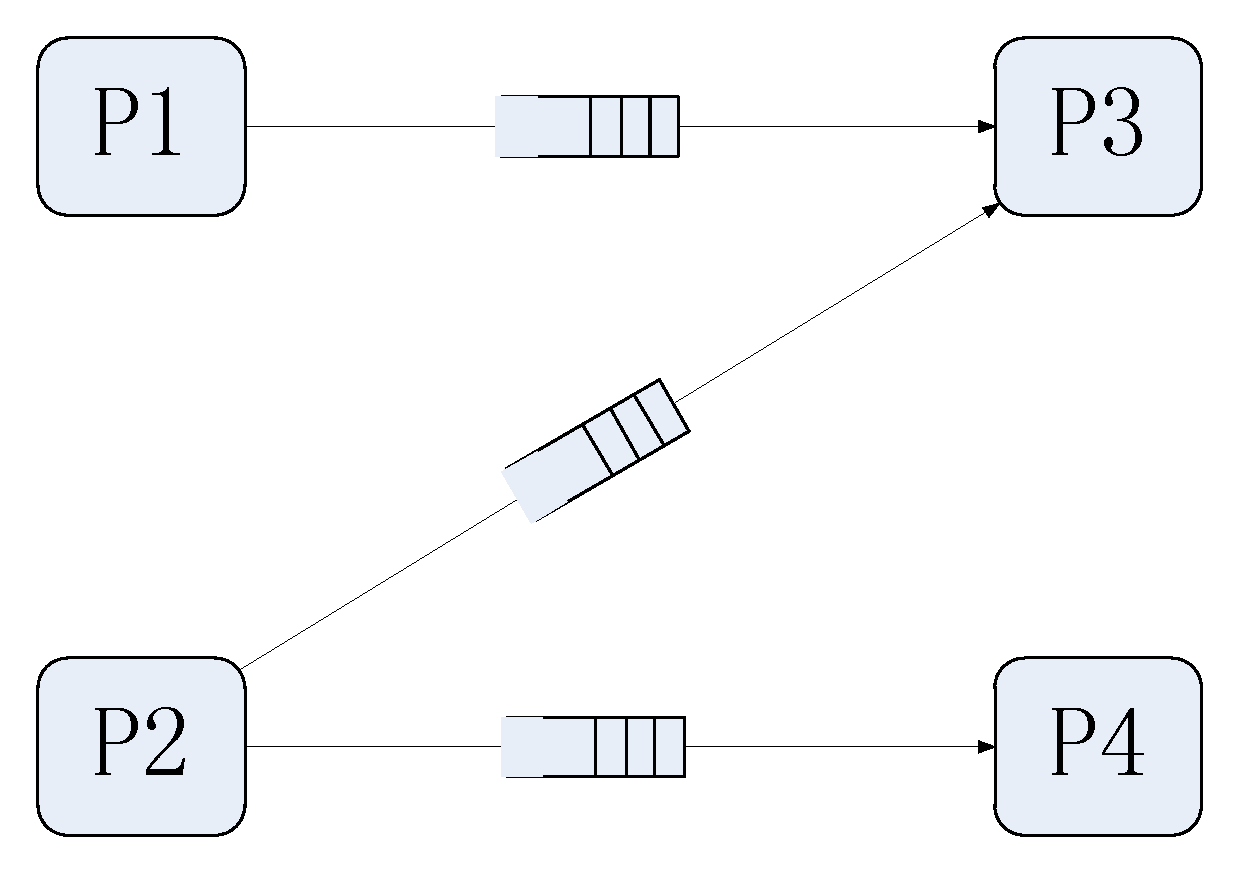
\includegraphics[height=20ex]{figure/basic-KPN.pdf}\\
  \caption{KPN 模型的例子}\label{basic-fig-KPN}
\end{figure}

同步数据流 (Synchronous Data Flow, SDF)\upcite{SDF1987} 是数据流模型的一种,在此模型中,运算单元每次执行时消耗与产生的数据量事先已知,因此系统执行时是可确定的,因此适用于静态调度,下一节将详细介绍。

此外,进程代数模型对进程之间的交互、同步通信机制提供了高层的形式化描述方法,此模型适用于分析、等价检查以及形式化验证。

\subsubsection{面向状态的计算模型}
在面向状态的计算模型中,具有代表性的几个模型有有限状态机 (finite state machines, FSM)、带数据的有限状态机 (finite state machines with data, FSMD) 等。此外,程序状态机 (Program State Machines, PSM) 可被视为一种组合了面向过程和面向状态两种类型的计算模型。这类模型多用于硬件实现层或者用于控制占主导的程序中,是动态调度的,在我们的算法中并不适合。


\subsection{SDF简介}
\label{SDF-intro}
% 简介 SDF 方法

%根据以上问题描述,以往的多核实时调度算法都不能很好的处理任务间数据依赖的约束,而DSP 中的SDF (Synchronous Data Flow)方法可以较好的描述任务间的数据依赖关系,因此可考虑用SDF的方法来解决以上问题。但SDF 方法不含有对实时任务时间约束的保证,因此需要对此方法加以改进。
在信号处理系统中,LGDF(Large grain data flow)用来表示DSP各计算单元间的数据流通。LGDF 是一个有向图,每个结点表示一个运算过程,可以是很小的运算单元,如加法器或乘法器,也可以是复杂的一段程序,如数字过滤器或FFT单元等。SDF来源于LGDF,但与之不同的是,SDF 要求每个运算单元的数据率在编译时是已知的,其中每条弧的起点表示数据出发结点一次运算所产生的数据,每条弧的终点表示数据接收结点每次运算所消耗的数据,如图\ref{basic-SDF-sample}。

\begin{figure}[!htb]
  \centering
  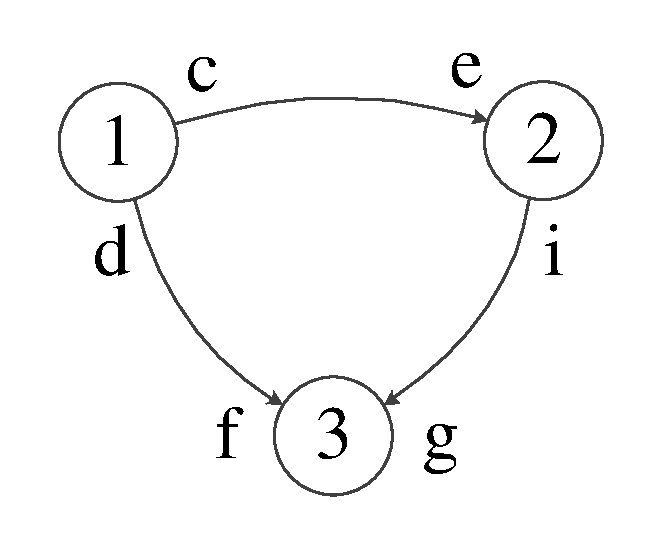
\includegraphics[height=15ex]{figure/basic-1-SDF.pdf}
  \caption{SDF图示例}
  \label{basic-SDF-sample}
\end{figure}

%\begin{figure}[!tb]
%\begin{floatrow}
%  {\ffigbox{\caption{SDF图示例}\label{basic-SDF-sample}} {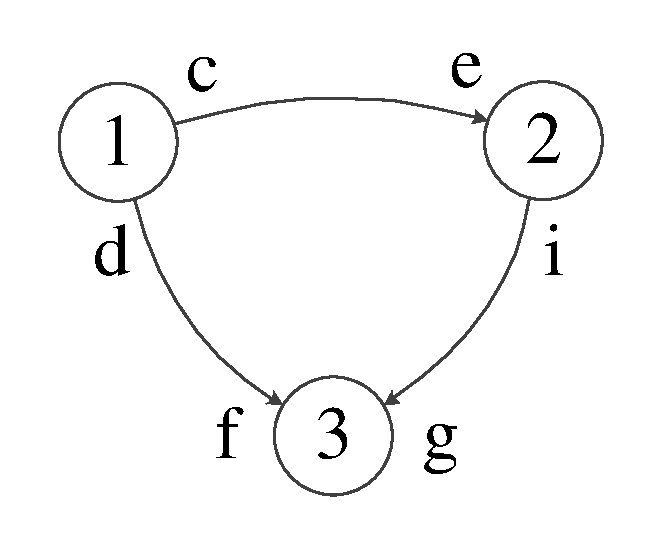
\includegraphics[height=15ex]{figure/basic-1-SDF.pdf}}}
%  {\ffigbox{\caption{SDF图中的Delay}\label{basic-SDF-Delay}}{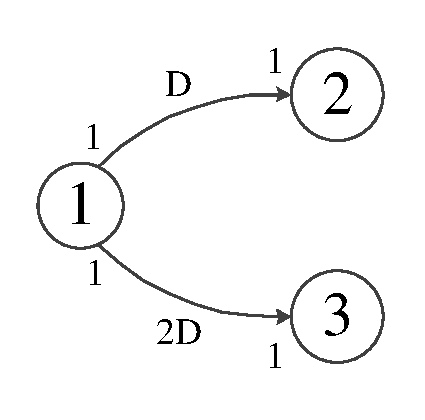
\includegraphics[height=15ex]{figure/basic-2-Delay.pdf}}}
%\end{floatrow}
%\end{figure}

图\ref{basic-SDF-sample}中从结点1到结点2的弧起点c表示结点1每运行一次在这条数据路径上产生c 单位的数据,而结点2 每运行一次在这条数据路径上消耗e 单位的数据。每个SDF 可用一个拓扑矩阵来表示,在矩阵中每列代表一个顶点,每行代表一条弧。如图\ref{basic-SDF-sample} 所示的SDF 图可由如下矩阵表示:

\begin{equation*}
  %\label{basic-SDF-matrix}
  \Gamma=\begin{bmatrix}
    c & -e & 0 \\
    d & 0 & -f \\
    0 & j & -g
  \end{bmatrix}
\end{equation*}

其中三列分别表示结点1、结点2和结点3,三行分别表示从结点1到结点2的弧、从结点1 到结点3 的弧和从结点2到结点3 的弧。由于每条弧上的两端结点运行不一定是完全同步的,因此每条弧上的数据会积累或减少,我们用向量b(n) 表示在n 时刻所有弧上的数据量,而向量

\begin{equation}
  v(n)=\begin{bmatrix}
    1 \\ 0 \\ 0
  \end{bmatrix} \textnormal{或}
  \begin{bmatrix}
    0 \\ 1 \\ 0
  \end{bmatrix} \textnormal{或}
  \begin{bmatrix}
    0 \\ 0 \\ 1
  \end{bmatrix}
\end{equation}

分别表示在n时刻运行1号结点或2号结点或3号结点。文章\cite{SDF1987} 证明了以上三者之间的关系为:

\begin{equation}
  \label{basic-eq-SDF}
  b(n+1)=b(n)+\Gamma{}v(n)
\end{equation}

弧上的Delay表示在系统开始运行前,该弧上已有多少有效数据。如图\ref{basic-SDF-Delay} 所示,在结点1 运行前,结点2 和结点3 分别可以运行1 次和2 次。

\begin{figure}[!htb]
  \centering
  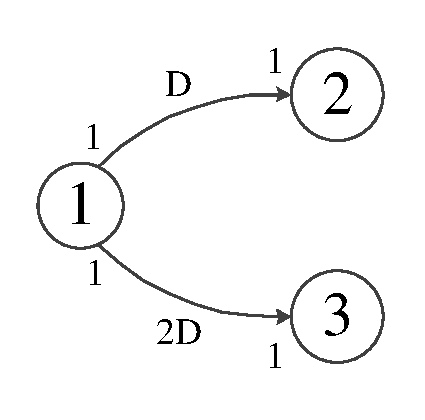
\includegraphics[height=15ex]{figure/basic-2-Delay.pdf}
  \caption{SDF图中的Delay}
  \label{basic-SDF-Delay}
\end{figure}

SDF图的Delay可以用初始时刻的b(0)向量来表示,它决定了系统可以怎样的顺序启动。如图\ref{basic-SDF-Delay} 的SDF图可以表示为

\begin{equation*}
  b(0)=\begin{bmatrix}
    1 \\ 2
  \end{bmatrix}
\end{equation*}

根据以上计算模型,假设SDF中结点数为s,文章\cite{SDF1987}证明了从SDF 图到单个处理器的一个可行的周期性串行调度(Periodic Admissible Sequential Schedule)存在的必要条件是

\begin{equation}
  \label{basic-eq-rank}
  \textnormal{rank}\Gamma=s-1
\end{equation}

由于调度是周期性的,在无限次循环的情况下,要使每条弧上的数据是一个有限值,只能使得一个周期结束后,所有弧上的数据量都回到周期开始前的状态。由\eqref{basic-eq-SDF} 式可知要满足此条件,必有

\begin{equation}
\label{basic-eq-matrix}
  \Gamma{}q=0
\end{equation}

其中向量q表示在每个周期内,每个结点的运行次数。根据以上方法,我们可以从一个SDF 图得到串行调度时每个周期内各个结点的运行次数。

但由此还无法得到一个可行的静态调度表,因为任务间有可能存在循环依赖关系。要打破循环依赖关系需要考虑将SDF转化为一个有向无环图(DAG),这要求我们首先弄清每个结点在运行时所需的数据要求哪些结点已经运行过足够的次数。假设在某SDF 图中有结点η到α的弧a,该SDF的拓扑矩阵为Γ,那么在α结点第j 次运行时,可以知道它所需的总数据量为$-j\Gamma_{a\alpha}$,弧a上原本有的数据为$b_a$,因此需要结点η 额外运行的次数为\upcite{SDF1987}

\begin{equation}
  \label{basic-eq-d}
  d_{\alpha\eta}=\left\lceil{\frac{-j\Gamma_{a\alpha}-b_a}{\Gamma{}_{a\alpha}}}\right\rceil
\end{equation}

才能够为α结点运行提供足够的数据。由以上\eqref{basic-eq-d}式可以得到从 SDF 图到 DAG 的一个S类算法\upcite{SDF1987},以解除SDF图中运算结点间的循环依赖关系。从DAG 再得到静态调度表则是NP完全问题,在运筹学上已经有所研究,目前主要用一些启发式算法,如 Hu-level 算法以及关键路径方法\upcite{HuLevel,CriticalPath}等。

此外,将任务调度到多个核上,生成静态调度表时,可以按照每个周期各结点的运行次数调度,也可按照J 个周期各结点的运行次数来调度。随着周期倍数J 的增大,得到的调度结果会越来越好。

%\emph{TODO}: 实例:一个 SDF 图的处理过程

\section{DAG调度算法简介}
\label{basic-DAG-sch}
% 简介从 DAG 到静态调度表的方法
% DLS 的主要思想

\subsection{DAG调度的分类}

从 DAG 到静态调度表的问题可分为以下四类\upcite{Comparison}:

BNP(Bounded Number of Processors):
    将 DAG 中的任务直接调度到固定个数的处理器上。处理器之间是全连接的。

UNC(Unbounded Number of Clusters):
    将 DAG 的任务调度到非限定个数的处理器上去。处理器之间是全连接的。这些算法采用的技术也称为 clustering

TDB(Task Duplication Based):
    将 DAG 的任务调度到非限定个数的处理器上去。使用任务复制技术来进一步降低完成时间。

APN(Arbitrary Processor Network):
    将任务调度到一个具有任意拓扑结构的处理器网络中去。

任务 DAG 是由一系列带有优先关系的原子任务所组成的有向无环图。一个任务结点可以有一个或多个输入,当所有输入都准备好后,该结点才可执行。在每条弧上有权重,表示从前一个任务结点到后一个任务结点的通信时间,当两个任务被分配至同一个处理器上时,该边的权重变为0。



由于我们需要考虑目标平台处理器多核之间的拓扑连接情况,而在以上四类现存算法中只有 APN 类是解决此类问题的,因此我们主要考察现存算法也主要来自这一类别。而 BNP 类算法要解决的问题是 APN 的子问题,其在解决问题的方法上有很大相似性,理解它们对解决 APN 类问题有很大帮助。

BNP 调度算法基于表调度方法。%解释表调度方法。
表调度方法中常用的图或结点的属性包括:t-level、b-level、static b-level、critical path 等\upcite{DistCompCH}:(假设$t_i$为图中的某个任务结点)% 分别解释
\begin{description}
  \item[t-level] 一个任务节点$t_i$的 t-level 属性是指从入口节点到$t_i$ (包括$t_i$) 的最长路径的长度。这里的路径长度是指这个路径上所有节点和边的权之和。
  \item[b-level] 一个节点$t_i$的b-level 属性是指从$t_i$到出口节点的最长路径的长度。所有节点的 b-level 都不会超过 DAG 的关键路径的长度。
  \item[static b-level] 一些算法在计算 b-level 的时候, 并没有考虑边权, 这样 b-level 在整个调度过程中都不会改变, 因而称为静态 b-level , 简写为SBL (Static B-Level)。
  \item[critical path] 关键路径 (Critical Path) 是一个DAG 图中最长路径。
\end{description}

BNP 中不同算法的区别主要在于针对以上属性,分配任务优先级时所采用的方法不同。有些对具有小 t-level 值的结点给与较高优先级,也有些使较大的 b-level 结点具有更高的优先级,还有些使用 b-level 与 t-level 的差值。总的来说,以 b-level 降序来调度结点,倾向于优先考虑关键路径上的任务结点;而使用 t-level 则倾向于以拓扑顺序来调度。而综合考虑 b-level 和 t-level 则产生介于以上两种情况之间的优先顺序。

    HLEFT (Highest Level First with Estimated Times)算法\upcite{HLEFT} 是一类最简单的算法,使用 static b-level 作为结点优先级。

    ISH (Insertion Scheduling Heuristic)算法\upcite{Kruatrachue1987} 将调度产生的空隙作为研究对象,向其中插入合适的任务结点。

    MCP (Modified Critical Path)算法\upcite{MCPScheduling}使用结点的 As-Last-As-Possible (ALAP) 属性作为优先级。在 CP 上的任务结点其 ALAP 值与 t-level 值相等。

    ETF (Earliest Time First)算法\upcite{ETFScheduling}每次重新计算所有可执行结点在所有处理器上的的最早开始时间来调度。

    DLS (Dynamic Level Scheduling)算法\upcite{DLS}使用 DL(Dynamic level)作为结点的优先级。DL 是结点的 static b-level 与其最早开始时间的差值。

    LAST 算法\upcite{LAST}不属于表调度算法,其主要目标是减少总的通信开销。

% 解决 DAG 问题的两种考虑 SBL 和 最早开始时间
%  DLS 的好处

APN 类算法考虑目标平台的特殊架构,如处理器数量、处理器之间的拓扑结构等。这类算法将任务调度到处理器上,并将消息传递调度到网络通信链路上,消息的调度可能取决于下层路由策略。此类中目前并没有太多算法\upcite{Comparison},下面主要讨论四种:

    MH(Mapping Heuristic)算法\upcite{MHScheduling}首先计算所有结点的 static b-level (SBL) 值,以 SBL 降序排列初始化一个 ready 结点列表,之后每个结点被调度到有最小开始时间的结点上。

    DLS(Dynamic Level Scheduling)算法\upcite{DLS},前面被分为 BNP 类算法,也可用作 APN 类算法。在用作 APN 类算法时,需要用户提供消息路由。

    BU(Bottom-Up)算法\upcite{BUScheduling} 首先寻找 DAG 的 Critical Path (CP),并将其中的所有结点都分配到同一处理器,然后将余下结点以拓扑的逆序分配给处理器,这些结点在分配时以处理器负载均衡为导向。

    BSA(Bubble Scheduling and Allocation)算法\upcite{BSA}以增量的方式逐渐形成一个优化的调度结果。首先将所有结点分配到一个枢轴处理器上(连接最多的处理器),然后算法试着将结点移到临近处理器上以提高每个结点的开始时间。枢轴处理器上所有结点都处理过后,将下一个处理器作为新的枢轴处理器。整个过程以宽度优先变换枢轴处理器不断重复,直到没有结点可被提前。

\subsection{DLS算法简介}
\label{basic-DLS-intro}

Dynamic Level Scheduling (DLS)算法\upcite{DLS}使用了一个动态层次 DL (Dynamic Level)作为任务调度排序的指标。DL 是一个结点的静态层数(SBL) 与它在一个处理器上的最早开始时间之差,相当于综合考虑了CP上的任务和 能够早开始的任务可以尽早开始 两方面情况。在调度的每个步骤中,算法要对在就绪池中的每个结点,计算它们在所有处理器上的 DL。 具有最大 DL 的结点-处理器对被挑选出来进行调度。其中在考虑各个任务于每个处理器上的最早开始时间时,需要根据下层路由得到消息在链路上的调度情况。

DLS算法的步骤如算法\ref{algo-DLS}所述,它的时间复杂度为 $O(n^{2}p f(p))$,其中$n$为 DAG 中的结点个数,$p$为处理器个数,$f(p)$是消息路由算法的时间复杂度。
% 待修改为算法格式
%\begin{Verbatim}[numbers=left,frame=single,xleftmargin=50pt]
%    (1)计算每个结点的 b-level 值
%    (2)初始化就绪结点池,使之包含所有入口结点。
%    反复执行以下步骤,直到所有结点调度完毕:
%        (2.1)计算每个结点在每个处理器上的最早开始时间,再将结点
%        的 SBL 减去最早开始时间,即计算出每个(结点-处理器)对的 DL
%        (2.2)选择具有最大 DL 的结点-处理器对,将该结点调度到相应
%        处理器上
%        (2.3)将最近的就绪结点加入到就绪池中
%\end{Verbatim}

\begin{algorithm}
\caption{DLS 算法}
\label{algo-DLS}
\KwIn{DAG 任务图,目标处理器平台}
\KwOut{静态调度表}
计算 DAG 中每个结点的 b-level 值 (SBL)\;
初始化就绪结点池 R,使之包含所有入口结点\;
\While{R 不空}{
    计算 R 中每个结点在每个处理器上的最早开始时间,再将结点的 SBL 减去最早开始时间,即计算出每个(结点-处理器)对的 DL\;
    选择具有最大 DL 的(结点-处理器)对,将该结点调度到相应处理器上\;
    将新的就绪结点加入到就绪池 R 中\;
}
\end{algorithm}


\section{分区系统简介}
\label{basic-partition}

在分区操作系统中,各个分区之间应该相互隔离,分区应为应用提供时间分区与空间分区。应用运行在系统为其提供的分区环境中,不受其他分区的影响。分区是分区操作系统分配资源的单位。

\subsection{分区、任务与处理器的关系}
% 以下几段来自赵纯毕设,最终提交前要改
分区的时间资源是指各个分区获得的处理器使用时间。运行于同一处理器上的所有分区共享此处理器的计算资源。分区系统需要保证分区能够获得固定的时间进而获得处理器的计算能力。操作系统以分区为单位分配处理器资源,在操作系统分配处理器资源时,并不感知分区内部的任务,即使一个分区内部不存在任务,那么操作系统也会将此处理器资源分配给相应分区,而不是分配给其他分区。同分区内的所有任务根据分区内任务调度算法共享分区的时间资源。分区系统需要保证分区不会使用其他分区的时间资源,这样系统能够保证分区的时间隔离。

分区空间资源是每个分区所有的地址空间。空间资源包括内存资源,I/O资源等。内存资源包括分区能够访问的虚拟地址空间和物理内存空间等,其中I/O资源包括分区能够访问的I/O 设备以及共享I/O设备中获得的带宽。空间资源由操作系统以分区为单位分配,分区间无共享资源,而分区内部的任务共享本分区内空间资源。

根据 ARINC 653 标准中关于分区与任务间关系的定义,分区是资源的分配单位,任务是系统的调度单位。应用通过任务来实现具体的功能操作,而分区为任务提供具体的分区环境与所需资源。一个分区内部可以有一个或者多个任务,而一个任务只能属于一个分区。

在分区与处理器的关系方面,ARINC 653 标准规定一个分区只能运行于一个处理器上,不允许分区在处理器之间迁移。分区与处理器之间的关系如图 \ref{basic-fig-partition} 所示。

\begin{figure}[!hbt]
  \centering
  % Requires \usepackage{graphicx}
  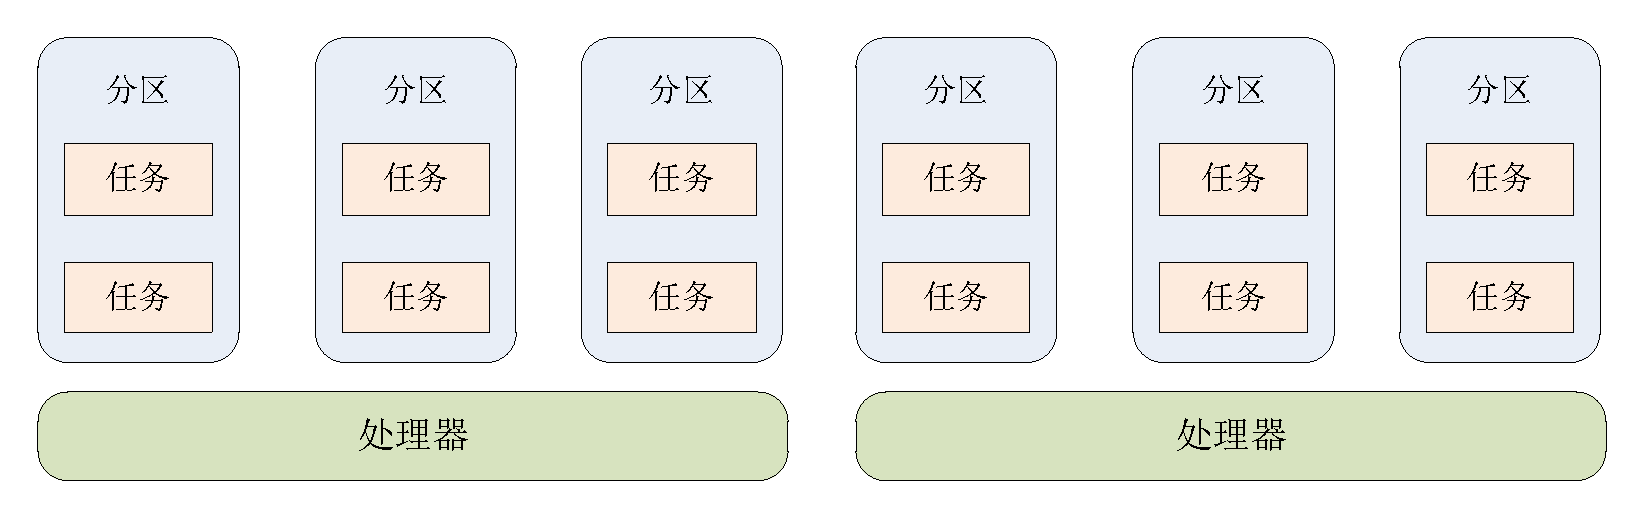
\includegraphics[height=25ex]{figure/basic-partition.pdf}\\
  \caption{分区与处理器的关系}\label{basic-fig-partition}
\end{figure}

\subsection{分区与任务调度的关系}

分区通过时间和空间两方面来实现,其中时间分区通过为各分区分配不同的处理器时间来实现,因此时间分区与调度系统直接相关。分区系统的调度通常分为两层,上层是处理器针对运行在其上的分区间调度,下层是各分区内部任务间的调度,两层可以各采用不同的调度策略。其中分区间调度可以是周期性的,也可以是非周期的,如果我们确切已知每个分区内部任务所需的总运行时间,则只需给每个分区分配其所需时间即可。

本文采用的是静态调度算法,在任务调度前即可知道任务数量、所有任务的时间信息等,因此可以根据任务属性,将所有任务均以分区隔离,每个分区内仅分配一个任务,使得任务与分区一一对应。这样即可使下层的分区内调度非常简单,分区内仅有一个任务,分区的运行时间即是分区内任务的运行时间。而上层调度所面对的各分区的时间属性与其内部所运行任务的时间属性相一致,因此上层针对分区的调度亦可认为是直接面向任务的调度,只需根据对应任务的时间属性分配即可。

\subsection{分区间通信}
\label{basic-partition-message}

处理器或核间通信可采用总线共享 Cache 或共享内存的方式来实现,也可采用片上互连的方式,如交叉开关或片上网络等。本文假定处理器或多核之间是基于片上互连的方案,各个处理器核心之间通过消息通信,其通信时间直接与通信数据量相关。如果核间消息传递速率为 s (即单位时间传递 s 的数据量),则传递 M 的数据需要 $M/s$ 的时间延迟。核间消息的传递是双向的,且同一个核可同时与多个与其有直接链路相连的核进行通信互不影响。

由于一个处理器或核上可以有多个分区,因此分区间通信包含同处理器上与不同处理器上的两种情况。同处理器上的分区间通信可直接通过缓存或共享内存来实现,本文假定其延时很小可忽略;而不同处理器上的分区之间通信则须采用处理器或核间通信的方式,如上段所述有一定延迟,并在此期间占用相应链路上的通信资源。

\section{本章小结}

本章主要介绍了与论文相关的理论与技术。首先对周期性与偶发实时任务模型的相关调度算法理论做了简单总结,从任务模型、时间约束、调度环境、单处理器及多处理器调度等方面做了讨论。其次介绍了多核平台下的几种计算模型及其各自的特点,并着重介绍了SDF 模型,这是论文中所述算法的切入点,然后简要介绍了从 SDF 图转化为 DAG 的一种 S 类算法。本章还介绍了从 DAG 生成静态调度表的现有算法分类,所解决的问题类型以及各自的特点,并着重介绍了可用于 APN 问题的 DLS 算法,它是从 DAG 得到最终的静态调度表的算法基础。本章最后对分区操作系统中的任务与分区的相关概念做了介绍。



% 改进的 SDF 算法
% !Mode:: "TeX:UTF-8"

\chapter{构建广义同步数据流图}
\label{chapter-SDF}

\section{COSS 算法简介}
% COSS 流程 及 优劣比较

\subsection{问题模型}

% 首先定义有效调度:
% 包括 任务调度表、消息调度表

首先对目标问题给出一个精确的描述。

(1)	给定一个任务集 $T=\{t_1, t_2, ..., t_n\}$。

(2)	对每个任务 $t_i$,存在两种可能的约束类型:时间约束或数据依赖约束,也可能两种约束都有。

(3)	任务 $t_i$的时间约束是指:任务的释放周期$T_i$、执行的相对时限$D_i$以及首次任务释放时间$O_i$。

(4)	任务的数据依赖约束是指:任务$t_i$与$t_j$之间存在数据依赖关系,每次$t_i$ 执行产生 $p_{ij}$ 个数据发送给 $t_j$ ,而每次 $t_j$ 执行消耗 $c_{ij}$ 个数据。初始时 $t_i$ 到$t_j$的 Delay 为 $D_{ij}$,表示系统启动时在 $t_j$ 第一次运行之前 $t_j$ 在这条依赖关系上有多少数据可用。

(5)	目标平台中处理器数目m(或核数),以及每两个核之间通信时单位时间传输的数据量 s。关于目标平台的抽象模型,在第 \ref{DLS-chapter-SSL} 章有更详细的描述。

针对以上问题,给出一个调度算法,此算法根据以上约束,生成任务集 T 在给定多核架构上的静态周期性调度表以及任务间通信在处理器之间链路上的调度表,使所有任务满足约束条件,或者在调度失败时给出无法调度的结果。



\subsection{算法流程}

% 来自 abstract
COSS 算法主要由三步构成:
\begin{enumerate}
   \item 从表示任务间数据流的 SDF 图构建含有虚拟数据和虚拟结点的广义同步数据流 (General Synchronous Dataflow, GSDF) 图,其同时反映了任务间的数据通信关系和时间约束。
   \item 提出 Improved Class S (ICS) 算法,将上一步中得到的 GSDF 转化为一个调度周期的有向无环图 (Directed Acyclic Graph, DAG),将每个任务的多次执行用不同结点表示,并去除任务间的循环依赖关系。
   \item 提出修改的动态层级调度 (Modified Dynamic Level Scheduling, MDLS) 算法将 DAG 中的任务结点分配至目标多核/处理器平台,得到每个核/处理器的任务调度表,并给出核/处理器之间链路上的通信调度。
 \end{enumerate}

COSS 算法的流程图如图\ref{SDF-fig-COSS-steps}所示。
\begin{figure}[!hbt]
  \centering
  
\includegraphics[height=14ex]{figure/SDF-COSS-steps.pdf}
  \caption{COSS 算法流程图}
  \label{SDF-fig-COSS-steps}
\end{figure}



% 来自 SDF改的特点、优势劣势.docx 总结

\subsection{算法特性}

\subsubsection{静态调度}

由离线调度的特征可知,对于实时任务,只能处理周期性任务,而对偶发性任务和非周期任务由于无法预知具体任务的释放时间,无法处理。

离线调度的优势在于,系统开始执行前就排出各个任务的具体调度表,并分配给每个处理器。处理器在具体调度时只需按照分配给自己的调度表执行即可,而不用在运行时占用较大的开销来动态计算调度。每个处理器只用处理自己核上的调度表这一特点和分区调度有些相似,但在允许任务 job-level 迁移的情况时(全局调度)需要处理不同处理器之间任务转移、上下文切换的问题。

离线调度的另一个优势是,调度结果对时间限的保证是容易验证的。尤其对于多处理器的系统,如果将任务间的优先关系放入 WCET 分析中来考虑将带来较大挑战。例如在最简单的分区调度系统上,一个处理器中任务的执行可能间接影响到另外一个处理器上对系统共享资源有竞争关系的另一个任务的执行。有文章指出,目前对这样复杂的硬件相互影响的关系还不存在静态分析方法\upcite{WCET}。


\subsubsection{灵活性}

COSS 算法的本质是将一种周期性和任务间(循环)依赖关系共存的约束转化为一个周期内任务多次执行之间的 DAG 关系,而并没有严格限制只能是分区调度或全局调度。属于分区调度还是全局调度取决于从DAG 到m 个同构多处理器平台的具体映射算法。
如果在映射中限制条件只能将相同任务执行在同一个处理器上,那么将产生分区调度的调度表。如果允许相同任务在不同处理器运行,但每次执行只能在一个处理器上,那么将产生允许 task-level 迁移的调度。%如果任务一次执行在一个处理器被抢占,然后到另一个处理器恢复执行,那么将产生 job-level 迁移的调度(全局调度)。

此外,COSS 算法可以是抢占或非抢占的。在允许抢占式的调度下,会产生更好的调度结果。在一些情况下,非抢占的可能无法找到有效调度。


\section{并行计算模型}

\subsection{同步数据流的优势}
如 \ref{basic-MoC} 节所述,针对多核并行调度问题,已存在一些计算模型。常用的并行计算模型(MoC)有KNP、SDF、FSM、PSM 等几种\upcite{FormalModelComp},% 分别介绍几段
相比其他几种计算模型来说,SDF 要求所有计算结点的数据流量必须预先指定,这是SDF 的最大特点和优势。体现在如下几个方面:
\begin{enumerate}
  \item 方便静态调度、静态检测和验证。通过预先确定各个运算结点的数据率,可以在系统运行前进行静态调度,并预估各个数据流通道的数据量大小及所需缓存的情况。并方便进行运行前的死锁检测和缓冲溢出检测,这相比其他计算模型是一个极大优势。
  \item 方便处理非一致数据率的情况。例如结点A运行3次产生的数据能够让结点B 运行2 次,这样的情况用SDF 处理起来非常方便,可直接在小调度周期内确定各运算结点的执行次数与每次执行的依赖序列。
  \item 预先指定数据率并按此构造 DAG 的方式为我们向其中加入时间约束条件提供了方便。
\end{enumerate}
%因此,我们采用 SDF 模型作为构建 COSS 调度算法第一步的基础。

\subsection{广义同步数据流}

在 SDF 中,连接两个结点的一条弧就决定了两结点间任务的一种数据依赖关系,或者称为优先依赖关系。如图\ref{SDF-fig-VArc}所示,在第一个图中,任务B的执行受到任务A的制约,A每运行完3次B 才能够运行1 次;在第二个图中,弧上的 2 Delay 使得B第一次运行只需等待A第一次运行结束即可开始,后面仍然保持A运行3次B运行1 次的制约条件;第三个图中弧上端点数字的改变使A 和B 的执行频率也随之发生变化,A与B之间也有不同的制约关系;同样在第四个图中随着 Delay 的改变,A、B在保持运行频率不变的情况下,任务的依赖关系稍有不同。

\begin{figure}[!hbt]
  \centering
  % Requires \usepackage{graphicx}
  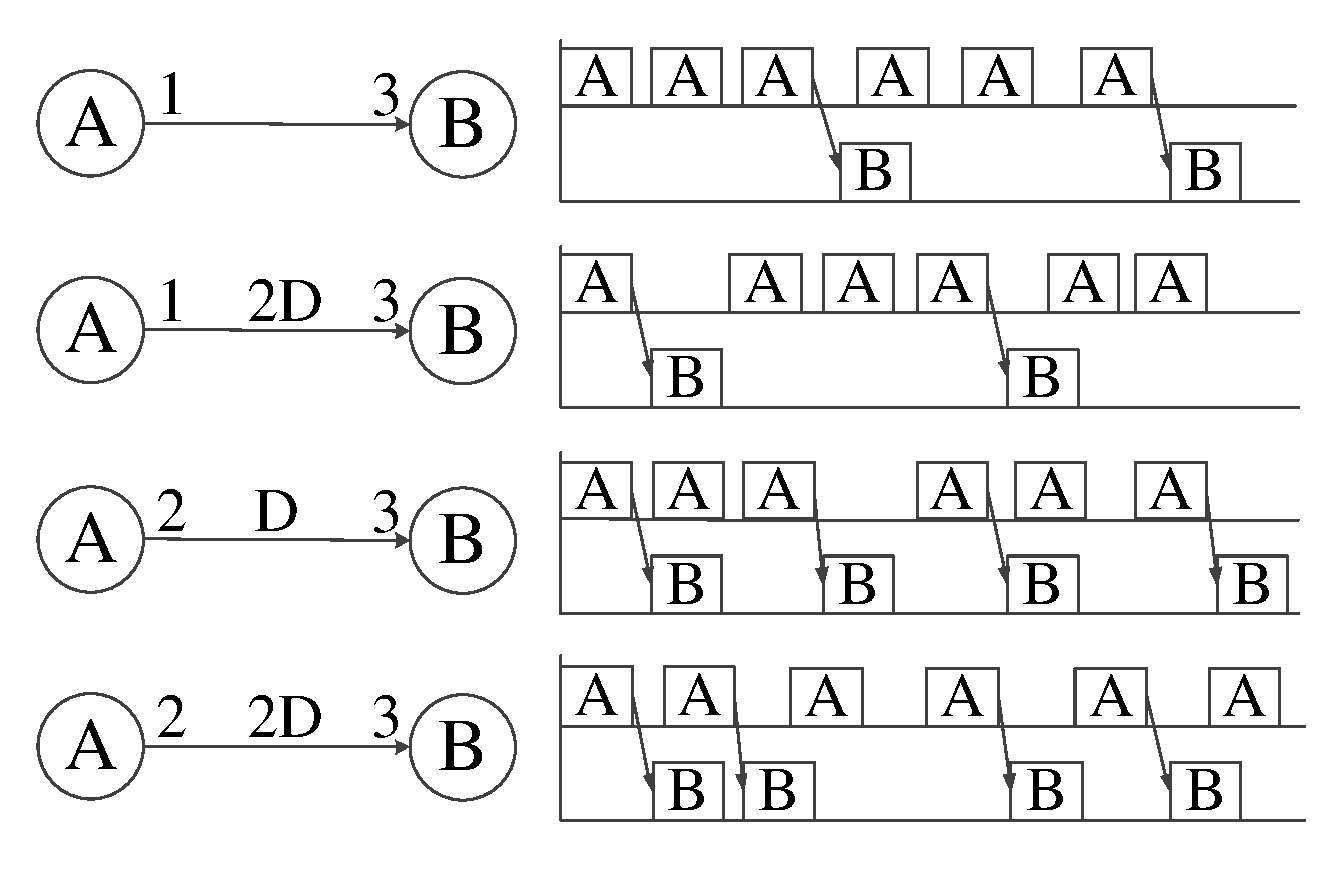
\includegraphics[height=30ex]{figure/SDF-VArc.pdf}\\
  \caption{SDF图中一些弧与优先关系的例子}\label{SDF-fig-VArc}
\end{figure}

从图\ref{SDF-fig-VArc}的例子可以看出,SDF 中不同的弧就对应了所连接两任务之间不同的制约关系。如果将弧上起点、终点的数字以及弧上的 Delay 都认为是虚拟数据,用这条弧表示一个虚拟数据流,那么该数据流也将决定任务间的一个优先依赖关系。而由于数据是虚拟的,其间并没有真正的数据通信,这样,如果要在已有的 SDF 任务之间加入新的优先依赖关系,那么只用向其中加入对应的虚拟数据流即可。本文称这类含有虚拟数据流的 SDF 为广义同步数据流 (General Synchronous Data Flow, GSDF)。

COSS 算法中对周期性释放时间和时间限的约束都是通过构建虚拟结点并在结点之间赋予特定的虚拟数据流来实现的。

%本算法的优势
\subsection{算法模型的选择}
COSS 算法选择SDF模型是因为SDF具有以下特点:

(1)	通过任务之间数据的产生和消耗值的设定,可灵活构建任务运行次数的比例关系。如$t_i$ -> $t_j$ 产生 m 个数据,消耗 n 个数据,可配比任务间运行频率为 n:m。 此产生和消耗的数据可以是真实的数据,也可是虚拟数据,如果是虚拟数据时,下一步从 DAG 构造静态表时不考虑数据通信的开销,只考虑任务间的运行次数比例及优先关系约束,可灵活实现各种任务间的优先关系。

(2)	将调度过程分为三步,构建 GSDF 图,从 GSDF 到 DAG,再从 DAG 生成静态调度表,也给该算法带来了灵活性。构建 GSDF 图的灵活性如(1)所述;此外,在从 DAG 到静态调度表前,还可根据特殊需求对 DAG 进行改动,使算法的使用范围更广(添加新的约束关系,改变任务间数据通信等)。此外,从 DAG 到静态调度表时任务是否可抢占也是可以灵活掌握的,如可在 DLS 算法中查找时间空隙时直接选取可最早开始的时间空隙,不足以完成任务时可继续使用下一时间空隙,有必要时还可将搜索策略由最早开始时间改为搜索最早结束时间等。


\section{释放时间约束}

在不考虑核间通信延时的情况下,由一个任务集数据依赖关系的SDF描述,可以得到在有限个核上的静态调度表。这离本文的目标还有一定的距离,因为任务的时间约束还没有处理。我们将时间约束分为任务周期性释放的时间约束和任务运行时间限 (deadline) 约束两部分分别处理。
%图\ref{SDF-fig-COSS-steps} 直观的给出目前待解决的问题存在于哪些过程,橙色底色的过程是研究的重点问题。

本节首先来考虑构建GSDF时,任务的周期性释放时间约束如何描述。它包括任务的释放周期$T_i$ 及首次任务释放时间$O_i$两方面。

\subsection{加入释放时间约束的方法}
\label{SDF-time-constraint}

在由任务集T根据约束关系构建SDF时,映射任务间数据依赖的约束关系是一件容易的事情,因为SDF本身就是描述数据在各运算结点间的流向的。首先在图中加入所有运算结点,然后按照SDF中弧的定义,依次加入所有任务间数据流向即可,弧上的数据反映有数据通信需求的任务间运行的频率比例。

下面重点考察周期性约束对SDF图的影响。由于SDF图是纯数据驱动型的,所有结点是否可调度完全取决于通向该结点的数据是否已准备充分,而实时系统中的周期性约束则完全是时间驱动型的。这样,要在SDF 中能处理时间层面上的问题,有必要在SDF中引入反应实际时间信息的单元。因此,考虑在SDF中加入一个虚拟的单位周期任务结点V,它要满足以下两个条件\label{SDF-V-conditions}

(1)	为了能够反映时间,V必须是串行执行的,并且相邻两次运行之间无时间间隔。

(2)	为了反映单位周期,V执行时间必须是1个单位时间。

由此可知V必须有一条自依赖的弧,以保证V的串行执行。从以上两个条件可知,虚拟结点 V 第k 次运行的释放时间为
\begin{equation}\label{SDF-eq-R0k}
  R_0[k]=k-1
\end{equation}
结束时间为
\begin{equation}\label{SDF-eq-F0k}
  F_0[k]=R_0[k]+1=k
\end{equation}

有了单位周期结点V 后,相当于整个SDF系统中有了标准时钟,假设任务$t_i$的释放周期和首次释放时间分别为$T_i$ 和$O_i$,那么只需在虚拟结点V和$t_i$ 结点间加入一条虚拟数据流,弧的起点为1,终点为$T_i$,弧上的 Delay 值设为
\begin{equation}
  \label{SDF-eq-r-time}
  D_{0i}=T_i-O_i
\end{equation}
即可,如图\ref{SDF-fig-time-constraint}所示,从 V 到 $t_i$ 的弧即为所添加的对 $t_i$ 的释放时间约束。

\begin{figure}[!hbt]
  \centering
  % Requires \usepackage{graphicx}
  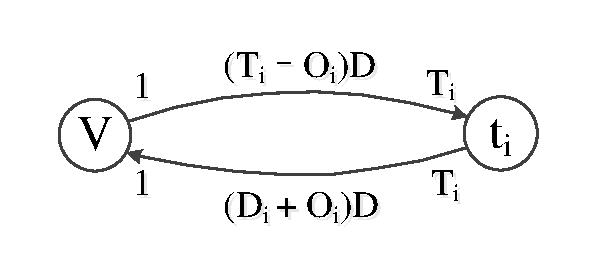
\includegraphics[height=13ex]{figure/SDF-time-constraint.pdf}\\
  \caption{在SDF中为$t_i$添加时间约束}\label{SDF-fig-time-constraint}
\end{figure}

%=======================================================================
%产生两个问题,一个是周期约束与数据约束的一致性问题,另一个如下所述


例如有以下周期性任务集 $T=\{t_1, t_2\}$,周期性时间约束为
\begin{gather*}
  t_1: T_1=2, O_1=0\\
  t_2: T_2=3, O_2=0
\end{gather*}

根据以上方法可以构建GSDF图如图\ref{SDF-fig-r-time}所示。

\begin{figure}[!htb]
  \centering
  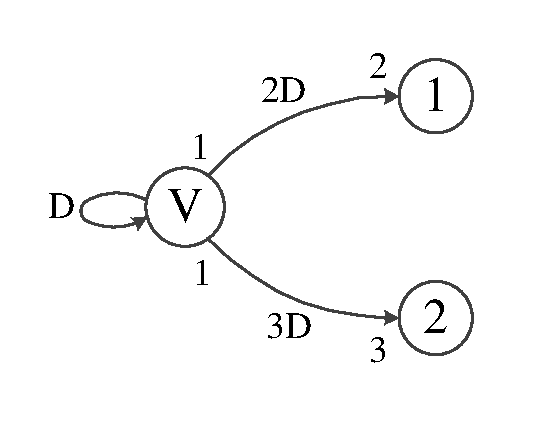
\includegraphics[height=20ex]{figure/SDF-1-r-time.pdf}
  \caption{一组周期性任务加入释放时间约束后得到的GSDF图}
  \label{SDF-fig-r-time}
\end{figure}

由于$O_1=O_2 = 0$,根据 \eqref{SDF-eq-r-time} 式得到两条弧上的 Delay 分别为2D 和3D。 该 GSDF 的拓扑矩阵为
\begin{equation*}
  \Gamma=\begin{bmatrix}
    1 & -2 & 0 \\
    1 & 0 & -3
  \end{bmatrix}
\end{equation*}
由此,根据 \eqref{basic-eq-matrix} 式可以解得周期内最小整数向量为
\begin{equation*}
  q=\begin{bmatrix}
    6 \\
    3 \\
    2
  \end{bmatrix}
\end{equation*}

以下按文献\cite{SDF1987}中的S类算法得到DAG如图\ref{SDF-fig-DAG} 所示。

\begin{figure}[!htb]
  \centering
  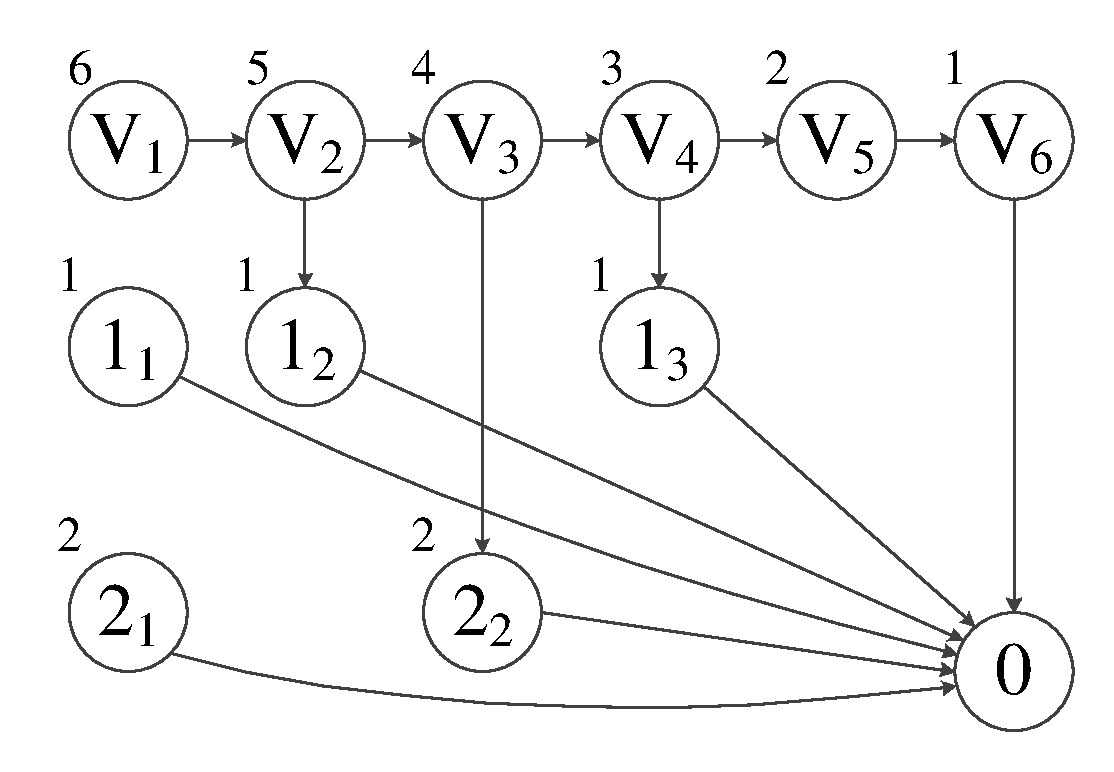
\includegraphics[height=22ex]{figure/SDF-2-DAG.pdf}
  \caption{一组周期性任务根据S类算法得到的DAG图}
  \label{SDF-fig-DAG}
\end{figure}

假设要将此任务集调度到2个处理器上,按照Hu-level的启发式算法\upcite{SDF1987} 可以得到如图\ref{SDF-fig-sch} 的调度结果。

\begin{figure}[!htb]
  \centering
  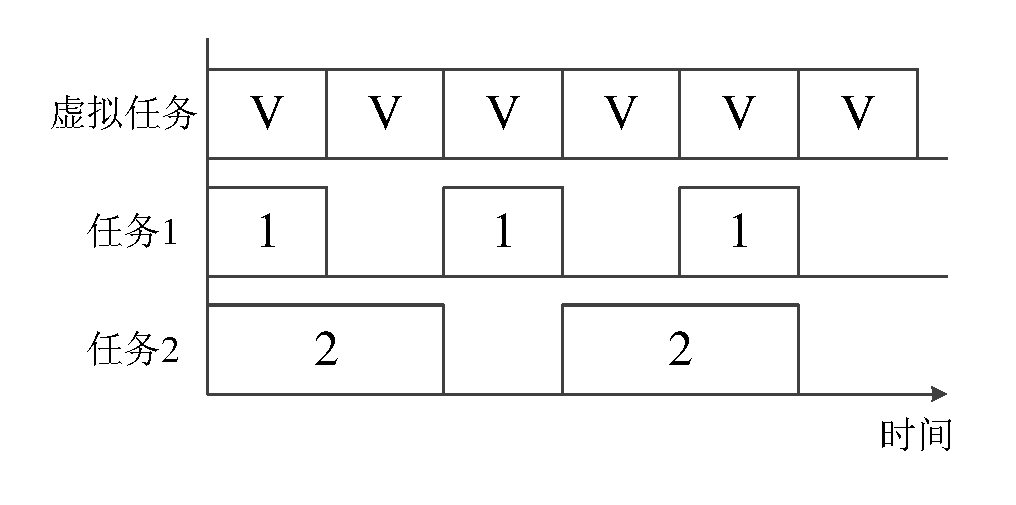
\includegraphics[height=20ex]{figure/SDF-3-sch.pdf}
  \caption{一组周期性任务根据DAG图分配到双核平台上的调度结果}
  \label{SDF-fig-sch}
\end{figure}

可以看到任务1和任务2分别满足了各自的周期性约束条件。

\subsection{加入时间约束的影响}
\label{SDF-time-constraint-influence}

加入时间约束会带来两个问题,首先是虚拟结点造成的影响,其次是关于时间约束与数据约束的一致性问题,以下分别讨论。

(1)加入虚拟结点产生的影响是,按正常调度算法将虚拟结点和其他普通运算结点一起调度的话,势必会使虚拟结点占用正常处理器的运算资源,而实际上这些都是闲置的。因此,在从DAG到生成静态调度表的过程中,也需对虚拟结点特殊处理,这将会在\ref{DLS-virtual-node}节详细论述。

(2)由于表述任务间数据关系的 SDF 图本身即表明了任务之间运行次数的比例关系,例如任务 A 到 B 的依赖关系中,A 每次产生 3 个数据,B 每次消耗 2 个数据,为了保证数据传输速率一致,两任务在调度周期内的运行次数比一定是 2:3 的关系。这样就要求我们在 A 和 B 上添加的周期性约束也必须符合两任务的运行次数比。例如将两任务的周期设为相同时,时间和数据约束的不一致性将导致任务无法调度。这个要求其实反映了 \ref{SDF-intro} 一节中 \eqref{basic-eq-rank} 式所描述的约束条件。如果任务的时间与数据约束不一致,将造成 GSDF 图的拓扑矩阵无零向量解。

但时间约束相比数据依赖约束并不是冗余的,它在任务之间运行次数比例关系以外对任务的释放与执行时间提出了新的要求。仍旧拿上一段中的例子来考虑,已知任务 A 与 B 在一个调度周期内的运行次数比例是 2:3,但如图 \ref{SDF-fig-consistent-constraint} 所示的两种运行分布都是符合数据依赖关系的,显然任务 $t_1$ 与 $t_2$ 不一定具有周期属性。在 (a) 图中任务 A 的两次运行都紧密排布于调度周期的开始,在 (b) 图中任务 B 的三次运行都处于调度周期的末尾,无论如何划分周期,它们都不可能成为周期运行的。

\begin{figure}[!hbt]
  \centering
  % Requires \usepackage{graphicx}
  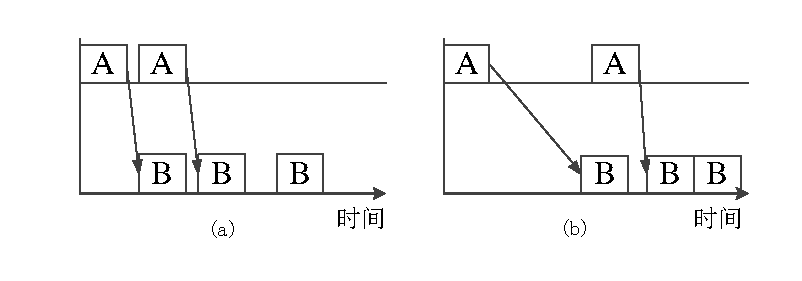
\includegraphics[height=18ex]{figure/SDF-consistent-constraint.pdf}\\
  \caption{SDF 中相同数据约束下的不同时间调度结果}\label{SDF-fig-consistent-constraint}
\end{figure}

但如果将任务 B 加入周期时间约束,就会产生类似图 \ref{SDF-fig-consistent-constraint-2} 所示调度结果,其中 B 在调度周期内仍均匀分布于三个小周期内,即同时符合了周期性与数据依赖关系。

\begin{figure}[!hbt]
  \centering
  % Requires \usepackage{graphicx}
  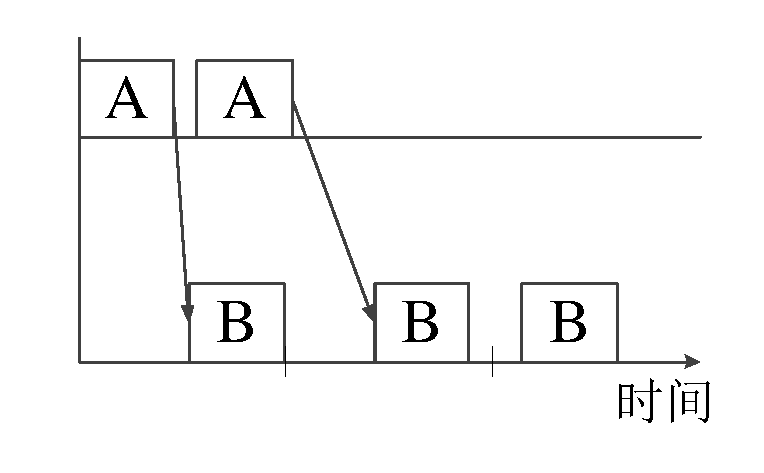
\includegraphics[height=15ex]{figure/SDF-consistent-constraint-2.pdf}\\
  \caption{SDF 中相同数据约束下的周期约束调度结果}\label{SDF-fig-consistent-constraint-2}
\end{figure}

综上所述,在 SDF 中添加周期约束是有必要的,且应与数据约束保持一致性。

\subsection{正确性证明}

下面对\ref{SDF-time-constraint}节所述方法的正确性给出证明。

%\emph{TODO}: 给出证明(待补全)
% 中期报告 + 英文小论文
由周期性任务时间限的定义可知,任务$t_i$第k次运行的释放时间为
\begin{equation}\label{SDF-eq-Rik}
  R_i[k]=(k-1)T_i+O_i
\end{equation}
根据 \eqref{basic-eq-d} 式可知,$t_i$的第k次运行依赖于虚拟结点的前
\begin{equation}\label{SDF-eq-di0k}
  d_{i0}[k]=\left\lceil\frac{T_ik-D_{0i}}{1}\right\rceil=(k-1)T_i+O_i
\end{equation}
次执行。再由 \eqref{SDF-eq-F0k} 式可知虚拟结点前 $d_{i0}[k]$ 次运行结束的时间为
\begin{equation}\label{SDF-eq-F0di0k}
  F_0[d_{i0}[k]]=d_{i0}[k]=(k-1)T_i+O_i
\end{equation}

从 \eqref{SDF-eq-Rik} 和 \eqref{SDF-eq-F0di0k} 式可以看出,$R_i[k]$ 与 $F_0[d_{i0}[k]]$ 相等,也即是说虚拟结点前 $d_{i0}[k]$ 次运行的结束的时间与任务 $t_i$ 第 k 次运行的释放时间相同,因此说明按前述方法在 GSDF 中加入的弧正确反映了任务 $t_i$ 在释放时间上的约束关系。



\section{时间限约束}

\subsection{加入时间限约束的方法}

时间限的约束相比周期性约束理解起来要复杂些。为了保证任务能够在规定时间内完成,仍然要将任务与作为系统时钟的虚拟结点V相联系,但这次需要使V限制任务的结束时间,因此需要从任务结点 $t_i$ 向虚拟结点 V 构建反向弧的制约关系。但这样只是有可能在生成静态调度表时使V在虚拟处理器的调度后移,虚拟处理器上对 V 的调度产生间隙,从而使 V 失去了作为系统时钟的功能。因此需要在下一阶段由DAG产生静态调度表时采用新的判断算法,一方面必须在满足所有约束条件的情况下将V 安排在虚拟处理器上,另一方面V之间的调度不能产生间隙,否则将不能保证实时任务对时间限约束的满足。

下面讨论具体将时间限约束加入SDF图的算法。假设任务 $t_i$ 的时间约束分别为 $T_i$,$D_i$ 和 $O_i$:在图中加入从结点$t_i$ 到虚拟结点V的弧,起点设为 $T_i$,终点为 1,并将弧上的 Delay 设为
\begin{equation}
  \label{SDF-eq-deadline}
  D_{i0}=D_i+O_i
\end{equation}
如图\ref{SDF-fig-time-constraint}所示,其中从 $t_i$ 到 V 的虚拟数据流即为添加的 $t_i$ 的时间限约束。


如有以下周期性任务集 $T=\{t_1, t_2\}$,周期性时间约束为
\begin{gather*}
  t_1: T_1=2, D_1=2, O_1=0\\
  t_2: T_2=3, D_2=3, O_2=0
\end{gather*}

根据前述方法可以构建 GSDF 图如图\ref{SDF-fig-deadline}所示。

\begin{figure}[!htb]
  \centering
  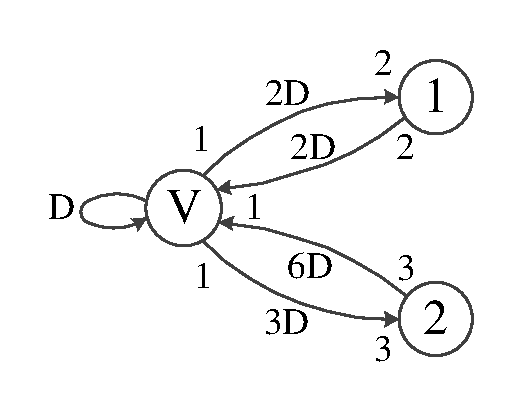
\includegraphics[height=20ex]{figure/SDF-4-deadline.pdf}
  \caption{在SDF图中加入时间限约束}
  \label{SDF-fig-deadline}
\end{figure}

\subsection{正确性证明}

下面证明此方法对实时任务时间限的保证。

%\emph{TODO}: 给出证明(待补全)
% 中期报告 + 英文小论文
由周期性任务时间限的定义可知,任务 $t_i$ 第k次运行的绝对时间限 (absolute deadline) 为
\begin{equation}\label{SDF-eq-Dik}
  D_i[k]=R_i[k]+D_i
\end{equation}

考察虚拟任务的第 $D_i[k]+1$ 次运行,由 \eqref{basic-eq-d} 式可知,它依赖于任务 $t_i$ 的前
\begin{equation}\label{d0iDik}
  d_{0i}[D_i[k]+1]=\left\lceil\frac{(D_i[k]+1)-D_{i0}}{T_i}\right\rceil=k
\end{equation}
次运行,即任务 $t_i$ 的第 k 次运行的结束时间一定不晚于虚拟任务第 $D_i[k]+1$ 次运行的释放时间。而从 \eqref{SDF-eq-R0k} 式可知,虚拟任务第 $D_i[k]+1$ 次运行的释放时间为
\begin{equation}
  R_0[D_i[k]+1]=(D_i[k]+1)-1=D_i[k]
\end{equation}
这与任务 $t_i$ 第 k 次运行的绝对时间限相等。因此,如果虚拟任务能够中间无间隔的被串行调度,那么任务 $t_i$ 的结束时间一定能够满足时间限 (deadline) 的约束。

\section{算法复杂度分析}

本章主要内容是从待调度任务的周期性约束和数据依赖约束生成 GSDF 图,按照以上所述方法,根据任务的周期属性和任务之间的数据依赖属性可直接构建出 GSDF 图中的一个顶点或一条边,因此假设建立图中的一个结点或一条边为一个基本操作。已知任务集中的任务个数为 n,其中周期性任务有 p 个,任务之间的数据依赖关系有 q 个,那么构建的 GSDF 图中,顶点数为 $V_G=n+1$,边数为 $E_G=q+2p$,由此得到总的操作数为
$$\textnormal{Op}=(n+1)+(q+2p)=n+q+2p+1$$
因此构建 GSDF 过程的时间复杂度为
$$O(V_G+E_G)=O(n+q+p)$$

COSS 算法总的复杂度将在\ref{COSS-complexity}节中得到。

\section{任务集的可调度性}
在\ref{SDF-time-constraint-influence}节中可以看到任务的时间和数据约束的不一致性将可能造成任务无法调度。下面讨论可调度任务集的必要条件。

由于 COSS 算法前两步对任务的描述主要采用 GSDF 图,而它在数学特性上与 SDF 是一致的,因此 GSDF 模型对任务集的要求与 SDF 的基本一致,主要有以下几点:
\begin{enumerate}
  \item 数据约束内部,以及数据约束与周期性时间约束之间应当是一致的,如 \ref{SDF-time-constraint-influence} 节所述。其数学上的表述即如 \ref{SDF-intro} 节的 \eqref{basic-eq-rank} 式,要使拓扑矩阵有零向量空间的非零整数解,拓扑矩阵的秩必须是 (结点数-1)。
  \item GSDF 中弧上的 Delay 必须保证任务能够持续运行。如图\ref{SDF-fig-requirement}所示的两个 GSDF,其拓扑矩阵显然满足第1 条约束,但由于弧上的 Delay 不足,导致任务无法启动。
\begin{figure}[!hbt]
  \centering
  % Requires \usepackage{graphicx}
  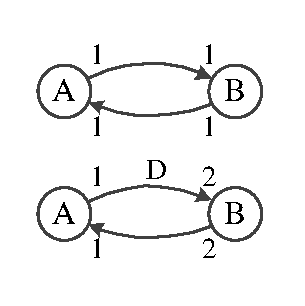
\includegraphics[height=22ex]{figure/SDF-requirement.pdf}\\
  \caption{Delay 不足导致 GSDF 任务无法启动}\label{SDF-fig-requirement}
\end{figure}

  \item \ref{SDF-time-constraint}节中对虚拟结点的约束也反映在任务的时间属性中。虚拟结点要求被串行且无间隔的调度,这要求在 GSDF 转化为 DAG 之后,所有虚拟结点的 SBL 以 1 为单位依次递减。如果虚拟结点的 SBL 值出现断层,则说明一定有任务在这些虚拟结点对应时间内的运行超过了时间限制,从而无法调度。
\end{enumerate}

任务集可调度的充分条件需要考虑目标平台的具体特征,如处理器的个数、连接情况、处理器之间传输速率等要素,无法确切得出,即使本调度算法对某一任务集无法找到有效调度,也不能下结论该任务集是不可调度的,可能存在有效调度只是算法没有找到,毕竟 DAG 的调度算法部分仅是一个启发式的算法,无法对所有可能的调度方案都一一搜索,那将会是 $O(n^m)$ 的复杂度。

\section{本章小结}

本章首先对 COSS 算法的总体设计给出了说明,包括要解决的问题模型、总体算法流程、研究过程中可能遇到的难点,并总结了 COSS 算法的优势所在。其次,本章第2节探讨了算法的构思过程,并论述了从几种并行计算模型中选择 SDF 模型作为算法切入点的原因,在此基础上提出了广义同步数据流模型,为在 SDF 图中灵活添加新的优先约束提供了条件。最后,本章从周期性任务的释放时间和时间限约束两方面分别论述了向 SDF 加入时间约束,构建 GSDF 图的方法,对方法的正确性给出了证明,并分析了算法的复杂度。



% ICS 算法,构建 DAG
% !Mode:: "TeX:UTF-8"


\chapter{广义同步数据流图转化为任务的有向无环图}
% ICS 算法
上一章得到了包含时间约束的 GSDF 图,下面需要生成对应的 DAG 图。通过 \ref{SDF-intro} 节中介绍的\cite{SDF1987}中的S类算法可以将GSDF转化为对应的DAG,但由于本文需要考虑通信问题,因此这个过程中也需要加入对数据的特殊处理。此外,虚拟结点在转化过程中也有其特殊含义。

\section{求解拓扑矩阵}
% 简述 从 GSDF 到 DAG 的过程
% 最小整数解中 q_0 的意义表示最小周期的长度

用 \ref{SDF-intro} 节中提到的方法可以得到 GSDF 图对应的拓扑矩阵 $\Gamma$。 为方便起见,假定 $\Gamma$ 的列的下标分别为 $0, 1, 2, \dots, n$,其中第 0 列对应的是虚拟结点,而 $1, \dots, n$ 列分别对应任务结点 $t_1, t_2, \dots, t_n$。 根据 \eqref{basic-eq-matrix} 式可以求得 $\Gamma$ 零向量空间的最小整数解为 $\textbf{q}$,其中虚拟结点所对应的 $\textbf{q}_0$ 即表示在一个最小周期中,虚拟任务将会被运行几次。根据 \ref{SDF-time-constraint} 节对虚拟结点所做的两点假定,可知虚拟结点在周期内一定串行且无间隔的连续执行,而每个虚拟任务的执行时间是单位时间,因此即有推论 $\textbf{q}_0$ 的值即为一个最小调度周期的长度。


\section{周期内结点间的数据传输}
\label{DAG-innerp}

SDF 图中任务之间数据吞吐速率可以是不同的,例如任务 A 与 B 之间,每次 A 执行产生 3 个数据,而每次 B 执行仅消耗 2 个数据,造成A 每次产生的数据需要分别传送给DAG图中B的两次不同的执行结点,这样才能够正确处理A、B 任务多次执行之间的消息传递。另外,在两个调度周期交界处,前一周期的任务结点也需要向后一周期的任务结点发送数据,且需要在前一周期结束前传输完毕,以使第二周期的任务在周期开始时能够回到与前一周期相同的状态,周期性调度才能够继续下去,因此也需要解决周期之间任务结点的数据传输问题。下面分别讨论。


本节讨论一般情况下周期内结点间数据传输的处理方式。现有任务$t_i$与$t_j$ 之间存在数据依赖关系,如图\ref{DLS-fig-gendep}所示,每次$t_i$ 执行产生 $p_{ij}$ 个数据,而每次 $t_j$ 执行消耗 $c_{ij}$ 个数据,初始时 $t_i$到$t_j$ 的 Delay 为 $D_{ij}$。

\begin{figure}[!hbt]
  \centering
  % Requires \usepackage{graphicx}
  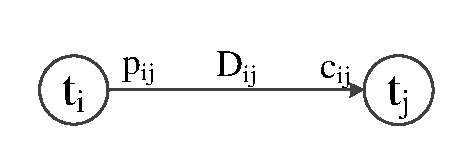
\includegraphics[height=8ex]{figure/DLS-gendep.pdf}\\
  \caption{SDF中$t_j$到$t_j$的一般依赖关系}\label{DLS-fig-gendep}
\end{figure}

需要解决的问题是求出$t_j$的第k次执行结点需要的数据分别来自$t_i$任务哪几次的运行结点,并求出分别需要的数据量是多少。从 \eqref{basic-eq-d} 式可以求得 $t_j$ 的第 k 次执行需要来自 $t_i$ 多少次执行的数据,但无法具体求出分别需要传输的数据量大小。为解决此问题,考察从 $t_i$ 到 $t_j$ 的数据量的对应关系,如图 \ref{DAG-fig-innerp-data} 所示。%如图所示。。。两行 分别表示产出 和 输入数据的对比图

\begin{figure}[!hbt]
  \centering
  % Requires \usepackage{graphicx}
  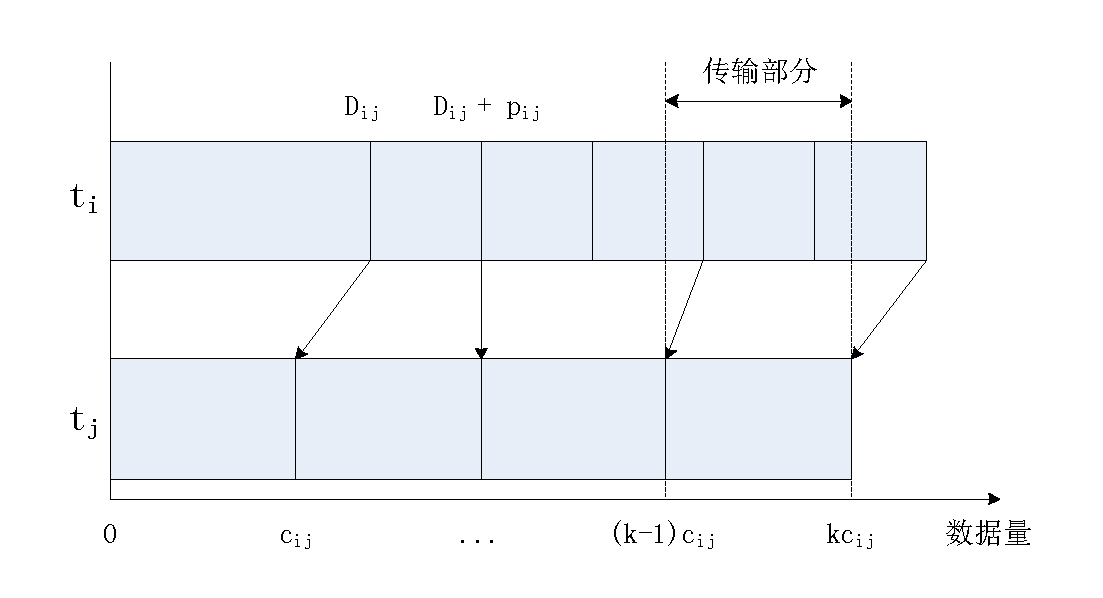
\includegraphics[height=30ex]{figure/DAG-innerp-data.pdf}\\
  \caption{DAG中$t_j$第k次运行与$t_i$的数据对应关系}\label{DAG-fig-innerp-data}
\end{figure}

任务 $t_j$ 的前k次执行共需数据量为
\begin{equation}
  \textnormal{Req}_{j}[k]=kc_{ij}
\end{equation}
前(k-1)次执行共需数据量为
\begin{equation}
  \textnormal{Req}_{j}[k-1]=(k-1)c_{ij}
\end{equation}
因此 $t_j$ 的第k次执行需要从 $(k-1)c_{ij}$ 到 $kc_{ij}$ 部分数据,如图 \ref{DAG-fig-innerp-data} 中虚线部分所示。下面来求这些数据与 $t_i$ 对应运行次数之间的数据关系,从图中可以看出,这部分数据来自 $t_i$ 与 $t_j$ 之间的 Delay 以及 $t_i$ 运行所产生的数据,即有
\begin{equation}\label{DAG-eq-innerp-eq1}
  D_{ij}+w_1p_{ij}+r_1=(k-1)c_{ij}
\end{equation}
和
\begin{equation}\label{DAG-eq-innerp-eq2}
  D_{ij}+w_2p_{ij}+r_2=kc_{ij}
\end{equation}
两式成立。其中 $r_1,r_2$ 表示边界情况时 $t_i$ 分别有部分数据需要传给不同的 $t_j$ 结点,$r_1,r_2$ 均为整数,且 $r_1\in[0,p_{ij})$ 而 $r_2\in[1,p_{ij}]$。
根据 \eqref{DAG-eq-innerp-eq1} 和 \eqref{DAG-eq-innerp-eq2} 式,以及以上对 $r_1,r_2$ 的约束可以解得
%\begin{equation*}
%  w_1=\left\lceil\frac{(k-1)c_{ij}-D_{ij}}{p_{ij}}\right\rceil
%\end{equation*}
%\begin{equation*}
%  r_1=(k-1)c_{ij}-D_{ij}-w_1p_{ij}
%\end{equation*}
%\begin{equation*}
%  w_2=\left\lceil\frac{kc_{ij}-D_{ij}-1}{p_{ij}}\right\rceil
%\end{equation*}
%\begin{equation*}
%  r_2=kc_{ij}-D_{ij}-w_2p_{ij}
%\end{equation*}
\begin{align}
  \label{DAG-eq-innerp-solve}
  w_1&=\left\lfloor\frac{(k-1)c_{ij}-D_{ij}}{p_{ij}}\right\rfloor\\
%  \label{DAG-eq-innerp-solve-2}
  r_1&=(k-1)c_{ij}-D_{ij}-w_1p_{ij}\\
%  \label{DAG-eq-innerp-solve-3}
  w_2&=\left\lfloor\frac{kc_{ij}-D_{ij}-1}{p_{ij}}\right\rfloor\\
  \label{DAG-eq-innerp-solve-ed}
  r_2&=kc_{ij}-D_{ij}-w_2p_{ij}
\end{align}

由以上四式可知,在边界条件下$t_i$的第$w_1$ 次运行需要传给$t_j$的第k次运行$p_{ij}-r_1$ 的数据量,而$t_i$的第$w_2$次运行需要传给$t_j$的第k次运行$r_2$的数据量。在边界条件中间的部分,每次 $t_i$ 运行产生的全部 $p_{ij}$ 数据都需要传给 $t_j$ 的第 k 次运行。当然,以上 $w_1$ 与 $w_2$ 也可能是相等的值,此时 $t_i$ 运行一次产生的数据量已大于 $t_j$ 的需求了,或者 $w_1<0$ 表示 $t_j[k]$ 结点有部分数据来自于 Delay 部分,这是下节要讨论的周期间数据传输的内容。

综上可知,$t_j$ 第 k 次运行的结点所需总数据满足以下关系:
\begin{equation}
  c_{ij}=(p_{ij}-r_1)+(w_2-w_1-1)p_{ij}+r_2
\end{equation}

根据以上所述内容,可以描述求出 $t_j[k]$ 结点依赖的周期内$t_i$结点数据传输量的过程如算法\ref{algo-DAG-innerp}所述。% 以后改为算法环境
\begin{algorithm}
  \caption{计算周期内结点间数据传输量}
  \label{algo-DAG-innerp}
  \KwIn{GSDF 图}
  \KwOut{DAG 中周期内结点间数据传输量}
  由\eqref{DAG-eq-innerp-solve}-\eqref{DAG-eq-innerp-solve-ed}四式求得 $w_1$、$r_1$、$w_2$ 和 $r_2$\;
  \uIf{$w_1==w_2$}{
      \If{$w_1 \geqslant 0$ AND $r_1 < r_2$}{
          添加从 $t_i[w_1+1]$ 到 $t_j[k]$ 结点的 $c_{ij}$ 大小的数据量\;
      }
  }
  \Else{
      \If{$w_1 \geqslant 0$}{
          添加从 $t_i[w_1+1]$ 到 $t_j[k]$ 结点的 $p_{ij}-r_1$ 大小的数据量\;
      }
      \For{$v=w_1+2$ TO $w_2$}{
          添加从 $t_i[v]$ 到 $t_j[k]$ 结点的 $p_{ij}$ 大小的数据量\;
      }
      \If{$w_2 \geqslant 0$}{
          添加从 $t_i[w_2+1]$ 到 $t_j[k]$ 结点的 $r_2$ 大小的数据量\;
      }
  }
\end{algorithm}

%\begin{Verbatim}[numbers=left,frame=single,xleftmargin=50pt,commandchars=\\\{\}]
%由上述四式求得 w1、r1、w2 和 r2。
%IF w1==w2 THEN
%    IF w1 >= 0 AND r1 < r2 THEN
%        添加从 ti[w1+1] 到 tj[k] 结点的 cij 大小数据量
%    END IF
%ELSE
%    IF w1 >= 0 THEN
%        添加从 ti[w1+1] 到 tj[k] 结点的 pij-r1 大小数据量
%    END IF
%    FOR v = w1 + 2 TO w2 DO
%        添加从 ti[v] 到 tj[k] 结点的 pij 大小数据量
%    END FOR
%    IF w2 >= 0 THEN
%        添加从 ti[w2+1] 到 tj[k] 结点的 r2 大小数据量
%    END IF
%END IF
%\end{Verbatim}

以上算法可加入 \cite{SDF1987} 所述的S 类算法过程中,在构造 DAG 的同时即可得到周期内结点间的具体数据传输量。在本章后面的小节中将给出一个包含了周期内数据传输以及周期间数据传输部分的改进的S 类算法,即 Imporved Class S Algorithm (ICS 算法)。


%\emph{TODO}: 给出周期内结点间数据传输的计算方法

\section{周期间结点间的数据传输}
\label{DAG-interp}

由于每个任务都需要将执行所产生的数据全部传输完毕才能保证下周期开始时系统回到相同的初始态,因此如果某个结点产生的数据向同周期内其他结点发送后仍留有剩余,那么该结点一定与下一周期内的任务存在数据传输关系,需要传输的数据量即为剩余的数据量。

另一方面,从GSDF图来看,只有$\textnormal{Delay}>0$的弧所指的结点在每周期开始时是有额外数据的,那么在周期间时,这些数据只能从上一周期的结点传来,因此周期间的数据传输只存在于GSDF图中由$\textnormal{Delay}>0$的弧所连接的结点之间。

仍然讨论一般情况下的处理方式,如图\ref{DLS-fig-gendep} 所示。任务$t_i$ 与$t_j$之间存在数据依赖关系,每次$t_i$执行产生 $p_{ij}$ 个数据,而每次 $t_j$ 执行消耗 $c_{ij}$ 个数据,初始时 $t_i$ 到$t_j$的 Delay 为 $D_{ij}$,且有 $D_{ij}>0$。

%\emph{TODO}: 给出周期间结点间数据传输的处理方法
Delay 是调度周期之间任务结点传输数据的缓冲区,因此跨周期传输的数据总量与GSDF 中所有弧上的 Delay 之和相等。针对上述一般情况,$t_i$ 任务结点在周期内产生的最后 $D_{ij}$ 个数据将会发送给下一周期 $t_j$ 所需前 $D_{ij}$ 个数据的任务结点,如图\ref{DLS-fig-interp} 所示。
\begin{figure}[!hbt]
  \centering
  % Requires \usepackage{graphicx}
  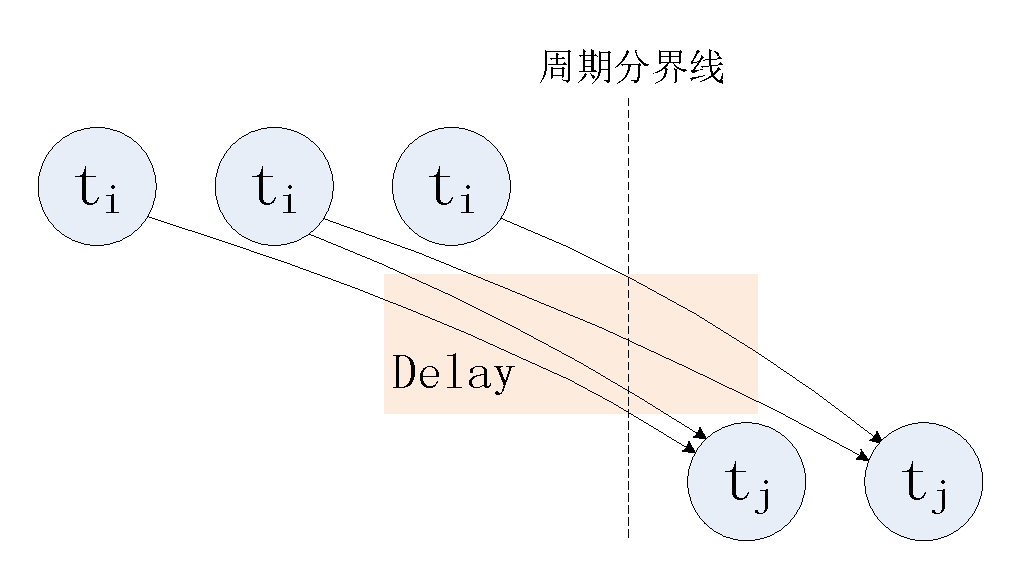
\includegraphics[height=20ex]{figure/DLS-interp.pdf}\\
  \caption{DAG周期间的数据传输关系}\label{DLS-fig-interp}
\end{figure}

明确了这个关系,就容易求得跨周期结点间的数据传输了。继续考察从 $t_i$ 到 $t_j$ 的数据量的对应关系,如图 \ref{DAG-fig-interp-data} 所示。

\begin{figure}[!hbt]
  \centering
  % Requires \usepackage{graphicx}
  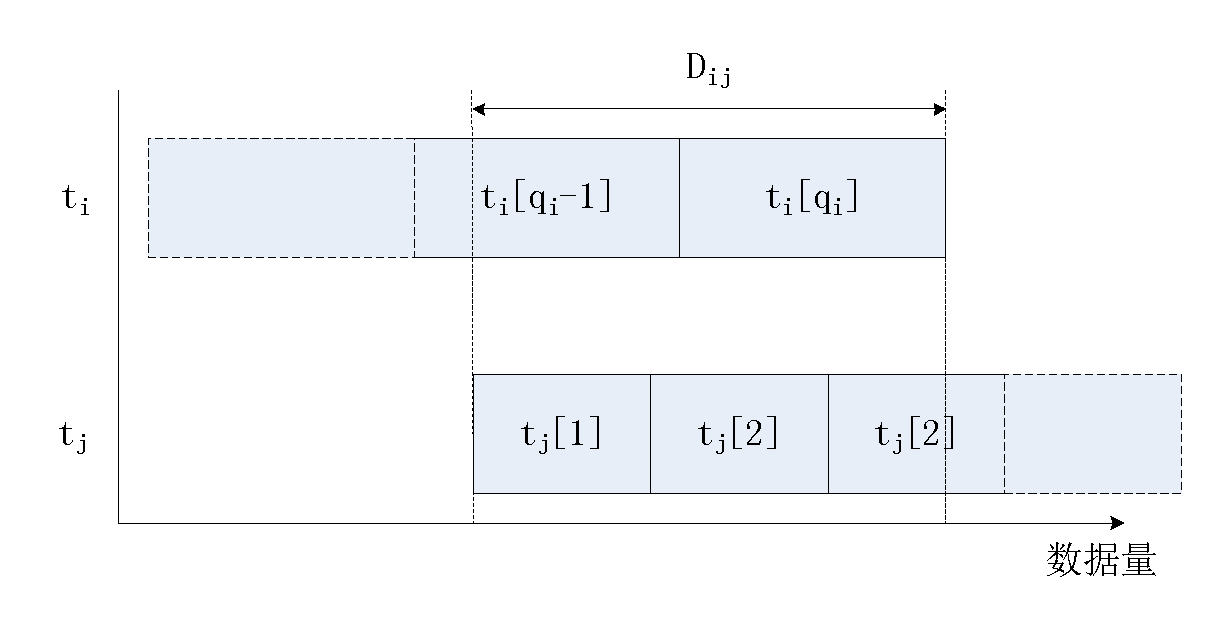
\includegraphics[height=25ex]{figure/DAG-interp-data.pdf}\\
  \caption{DAG中$t_i$与$t_j$周期间的数据对应关系}\label{DAG-fig-interp-data}
\end{figure}

注意到周期内 $t_i$ 的最后 $\left\lceil\frac{D_{ij}}{p_{ij}}\right\rceil$ 个结点发出的最后 $D_{ij}$ 个数据构成了跨周期的 Delay 部分,这些数据根据对应关系将会传给下一周期 $t_j$ 的前 $\left\lceil\frac{D_{ij}}{c_{ij}}\right\rceil$ 个结点。% 补充具体数据对应
与周期内结点间数据的处理方式不同,由于图 \ref{DAG-fig-interp-data} 中 Delay 部分对应数据在 $t_i$ 和 $t_j$ 上没有统一的起止点,无法由单一公式简单描述,只能从一端起逐个考虑 $t_i$ 结点与 $t_j$ 结点之间的数据传输关系。

根据图 \ref{DAG-fig-interp-data} 中 Delay 与 $t_i$ 部分的对应关系,可以求得 $t_i$ 从第
\begin{equation}\label{DAG-eq-interp-solve-w}
  w_i=q_i-\left\lceil\frac{D_{ij}}{p_{ij}}\right\rceil+1
\end{equation}
次运行开始将部分数据作为 Delay 部分传给下一周期的 $t_j$ 结点。该 $t_i$ 结点所要传输的数据大小为
\begin{equation}\label{DAG-eq-interp-solve-r}
  r_{i1}=D_{ij}-(w_i-1)p_{ij}
\end{equation}
而接收数据的 $t_j$ 的第一个结点  $t_j[0]$  需要 $c_{ij}$ 的数据,比较 $r_{i1}$ 与 $c_{ij}$ 的大小,即可知道需要将 $t_i[w_i]$ 结点产生的 $r_{i1}$ 数据部分还是全部传给 $t_j[0]$ 结点。如果 $r_{i1}>c_{ij}$,那么将 $c_{ij}$ 大小的数据传给 $t_j[0]$ 结点,剩余的 $$r_{i2}=r_{i1}-c_{ij}$$ 数据继续向后面的 $t_j$ 结点传送;而如果 $r_{i1}<c_{ij}$,那么 $r_{i1}$ 需要全部传给 $t_j[0]$ 结点,并且还需继续考察后面 $t_i[w_i+1]$ 结点所产生的 $$r_{i2}=p_{ij}$$ 有多少需要传给 $t_j[0]$ 结点……持续以上过程,直到所有 $D_{ij}$ 的数据全部分析完毕,即可求得跨周期的 $t_i$ 与 $t_j$ 结点之间分别有多少数据需要传输。

%下面将以上过程给出较详细的算法描述:
算法 \ref{algo-DAG-interp} 将以上过程给出了较详细的描述。
\begin{algorithm}
  \caption{计算两任务周期间结点间数据传输量}
  \label{algo-DAG-interp}
  \KwIn{GSDF 图}
  \KwOut{DAG 中周期间结点间数据传输量}
  由 \eqref{DAG-eq-interp-solve-w} 和 \eqref{DAG-eq-interp-solve-r} 两式求出 $w_i$ 和 $r_i$\;
  $w_j=0$\;
  $r_j=c_{ij}$\;
  \While{$w_i \leqslant q_i$}{
      \uIf{$r_i < r_j$}{
          trs = $r_i$\;
          添加从 $t_i[w_i]$ 到 $t_j[w_j]$ 结点 trs 大小的数据量\;
          $r_i=p_{ij}$\;
          $w_i=w_i+1$\;
          $r_j=r_j -$ trs\;
      }\Else{
          trs = $r_j$\;
          添加从 $t_i[w_i]$ 到 $t_j[w_j]$ 结点 trs 大小的数据量\;
          $r_j=c_{ij}$\;
          $w_j=w_j+1$\;
          $r_i=r_i -$ trs\;
      }
  }
\end{algorithm}

%\begin{Verbatim}[numbers=left,frame=single,xleftmargin=50pt,commandchars=\\\{\}]
%由以上两式求出 wi 和 ri
%wj = 0
%rj = cij
%WHILE wi <= qi DO
%    IF ri < rj THEN
%        trs = ri
%        添加从 ti[wi] 到 tj[wj] 结点的 trs 大小数据量
%        ri = pij
%        wi = wi + 1
%        rj = rj - trs
%    ELSE
%        trs = rj
%        添加从 ti[wi] 到 tj[wj] 结点的 trs 大小数据量
%        rj = cij
%        wj = wj + 1
%        ri = ri - trs
%    END IF
%END WHILE
%\end{Verbatim}

由以上算法即可容易求得 $t_i$ 到 $t_j$ 结点间跨周期的数据传输量。对 GSDF 内所有 Delay > 0 的结点之间如此进行即可求得所有跨调度周期结点间的数据传输量。

\section{改进的S类算法}
\subsection{算法流程}
结合以上两节周期内与周期间数据传输的不同处理方式,提出改进的S类算法 (ICS 算法)如算法 \ref{algo-ICS} 所述。
\begin{algorithm}
  \caption{Improved Class S (ICS) 算法}
  \label{algo-ICS}
  \KwIn{GSDF 图}
  \KwOut{DAG 中结点间数据传输量}
  求解 GSDF 对应的拓扑矩阵,得到零空间最小整数解向量 $q$\;
  建立初始 DAG 图\;
  向量 $e = 0$\;
  计算初始各边的 buffer 值得到向量 $b$\;
  建立 ready 任务集合 S,根据 $b$ 将满足输入条件的结点加入 S\;
  \While{S 不空}{
      从 S 中取出结点 i\;
      $e_i=e_i+1$\;
      在 DAG 中建立 i 的结点 $t_i[e_i]$\;
      根据 \ref{DAG-innerp} 节算法求出周期内结点间数据通信关系\;
      由 \eqref{basic-eq-SDF} 式更新 $b$\;
      \For{所有根据 $b$ 所得满足输入条件且不在 S 中的结点 $j$}{
          \If{$e_j < q_j$}{
              将结点 $j$ 加入 S\;
          }
      }
  }
  根据 \ref{DAG-interp} 节算法得到所有跨周期结点间数据通信关系\;
\end{algorithm}

%\begin{Verbatim}[numbers=left,frame=single,xleftmargin=50pt,commandchars=\\\{\}]
%求解 GSDF 对应的拓扑矩阵,得到零空间最小整数解向量 q
%建立初始 DAG 图
%向量 e = 0
%计算初始各边的 buffer 值得到向量 b
%建立 ready 任务集合 S,根据 b 将满足输入条件的结点加入 S
%WHILE S 不空 DO
%    从 S 中取出结点 i
%    ei = ei + 1
%    在 DAG 中建立 i 的结点 ti[ei]
%    根据第 2 节算法求出周期内结点间数据通信关系
%    由 2.2 式更新 b
%    FOR 所有根据 b 所得满足输入条件且不在 S 中的结点 j
%        IF ej < qj THEN
%            将结点 j 加入 S
%        END IF
%    END FOR
%END WHILE
%根据第 3 节算法得到所有跨周期结点间数据通信关系
%\end{Verbatim}

以上算法是在 \cite{SDF1987} 所述S类算法基础上改进而成,在将 GSDF 转化为 DAG 的同时还求出了每个运行结点与同其有数据依赖关系的结点之间的通信数据量,包括周期内的和周期之间的通信关系,因此称为改进的S类算法 (Improved Class S, ICS 算法)。

\subsection{复杂度分析}
假设 GSDF 图中顶点数为 $V_G$、边数为 $E_G$,转化出的 DAG 中顶点数为 $V_D$、边数为 $E_D$。
求解 GSDF 拓扑矩阵时,由于矩阵具有特殊性,结点之间是两两产生联系的,因此只用一遍深度优先遍历即可求得最小整数向量,最后再对得到的 $V_G$ 维向量归一化,复杂度为 $O(E_G+V_G)$。计算初始各边 buffer 值需对 GSDF 中各边依次进行,因此复杂度是 $O(E_G)$。

在循环过程中,建立结点的操作一共进行了 $V_D$ 次,复杂度为 $O(V_D)$。
求出周期内与周期间结点间的数据通信关系的过程,将得到 DAG 中所有边上的通信数据量,因此该步的复杂度为 $O(E_D)$。此外,对 GSDF 中每个结点的更新 b 的操作,相当于总的来说对 GSDF 所有边进行一次操作,因此复杂度为 $O(E_G)$。

综上,ICS 算法总的复杂度为 $$O(E_G+V_G)+O(E_G)+O(V_D)+O(E_D)+O(E_G)=O(E_G+V_G+E_D+V_D)$$



\section{本章小结}

本章设计了 COSS 算法的第二步,分析了从 GSDF 转化为 DAG 的方式,以及其过程中所遇到的周期内与周期间的数据传输量计算问题。本章分两节针对以上两个问题分别提出了解决方案,提出了 ICS 算法并详述了算法过程。通过 ICS 算法可以将上一章所得到的 GSDF 转化为对应的包含结点间数据传输量(带权)的DAG,为下一步得到最终的调度表做准备。



% 改进的 DAG 及 DLS 算法
% !Mode:: "TeX:UTF-8"

\chapter{生成调度表}
\label{DLS-chapter-SSL}

% 路由策略、调度策略(抢占、非抢占)、任务分配

COSS 算法的下一步需要从 DAG 生成最终任务和消息的调度表,除了面对一般的 DAG 调度问题外,在这个过程中,需要面对如下几个特殊问题:
\begin{description}
  \item[目标平台抽象] 本文调度的目标平台是多核分区操作系统。任务是系统调度的基本单位,而任务又必须在分区中执行,每个处理器上有多个分区,如何处理这三者间的关系是首先要考虑的问题。
      %从 DAG 到调度表的算法默认需要用户提供路由信息。因此,首先需要针对目标多核处理器平台,分析核间拓扑连接的关系,确定消息路由的策略。本文将考虑静态和动态路由两种方案,并分析其特点。
  \item[任务分配] %包括处理器排序 和 MH、DLS、BSA 算法的选择
      任务分配需要考虑三个问题:按怎样的顺序分配任务、将任务分配到哪个处理器核心的哪个分区上去运行以及任务如何调度(可抢占或非抢占式)。以下小节将从这几方面分别讨论。
  \item[虚拟结点] 与一般 DAG 调度不同的是,从 GSDF 得到的 DAG 中还包括一些并不需要真正执行的虚拟任务结点,它们与其他任务结点之间的数据传输也仅仅作为保证优先关系的手段而存在,并不会真的传递数据。因此在本文的算法中,针对虚拟结点也需要特殊处理。
\end{description}

下面将分小节分别讨论以上提到的问题。

\section{目标平台抽象}

本文调度的目标是多核处理器平台,处理器之间可以是全连接或部分连接的。如图 \ref{DLS-fig-connect}所示,(a)显示了4个处理器之间全相连的情况,(b)则是4 个处理器构成的一个环状网络,(c) 由5各处理器连成了不规则形状。处理器之间的连接情况由连接矩阵 C 表示,$C_{ij}=1$ 表示处理器 i 和 j 之间有链路直接相连,由于处理器之间链路是双向的,因此 C 是一个对称矩阵。以下三个矩阵分别对应图 \ref{DLS-fig-connect} 中 (a)、(b) 和 (c) 的连接情况。

\begin{gather*}
  C_1=\begin{bmatrix}
      -1 & 1 & 1 & 1 \\
      1 & -1 & 1 & 1 \\
      1 & 1 & -1 & 1 \\
      1 & 1 & 1 & -1
  \end{bmatrix},\quad
  C_2=\begin{bmatrix}
      -1 & 1 & 1 & 0 \\
      1 & -1 & 0 & 1 \\
      1 & 0 & -1 & 1 \\
      0 & 1 & 1 & -1
  \end{bmatrix},\quad
  C_3=\begin{bmatrix}
      -1 & 0 & 1 & 0 & 0\\
      0 & -1 & 1 & 0 & 0\\
      1 & 1 & -1 & 1 & 0\\
      0 & 0 & 1 & -1 & 1\\
      0 & 0 & 0 & 1 & -1
  \end{bmatrix}
\end{gather*}

\begin{figure}[!hbt]
  \centering
  % Requires \usepackage{graphicx}
  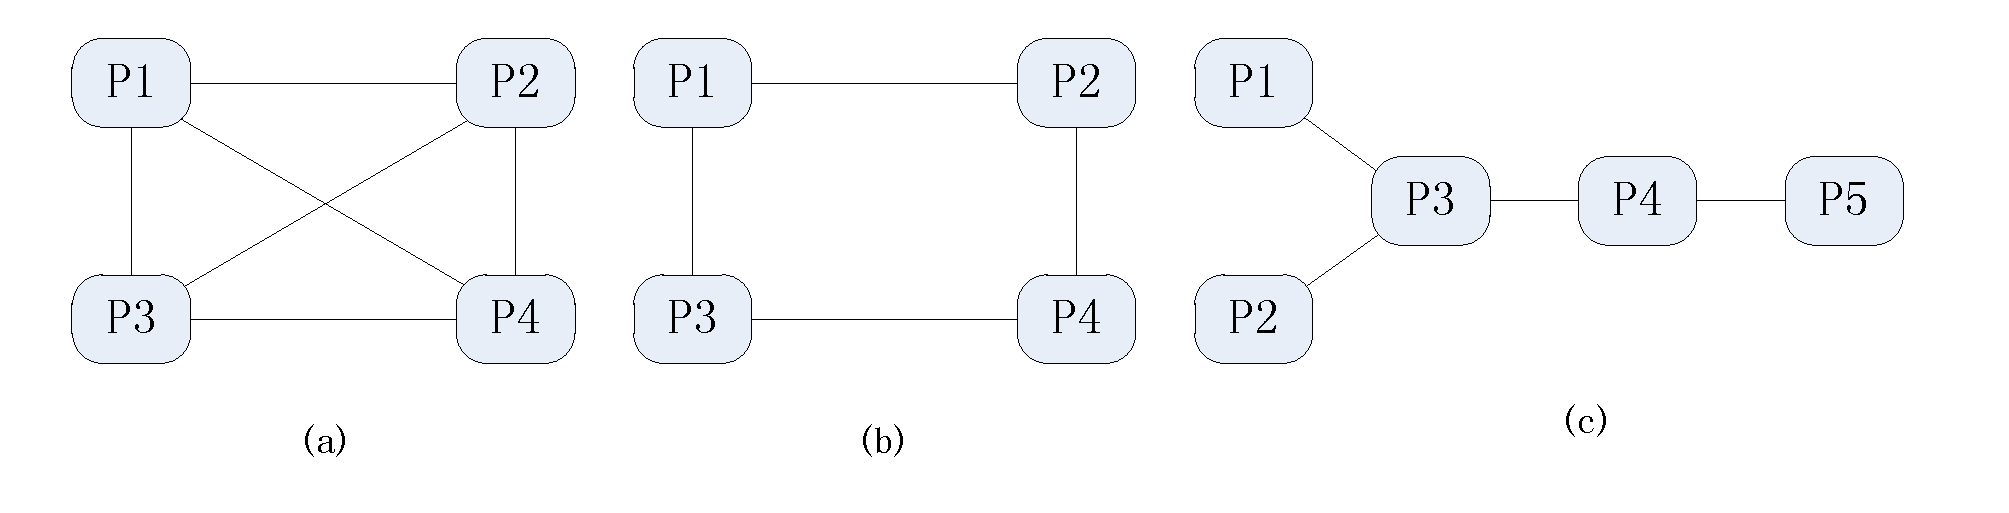
\includegraphics[height=17ex]{figure/DLS-p-connect.pdf}\\
  \caption{处理器连接示例}\label{DLS-fig-connect}
\end{figure}

本文假定直接相连的处理器之间具有相同的数据传输速率。没有链路直接相连的处理器之间在传输消息时需要通过其他处理器间接传递,消息的路由由平台本身给出。为输入方便,本文假定处理器之间消息的传递是静态路由,即具有相同起点和终点的消息通过相同的路径传递,消息传递选择具有最小跳数的路径。处理器间的路由信息由下一跳矩阵 H 给出,矩阵中 $H_{ij}$  表示当消息从处理器 i 要发往 j 时,要将其发往 $H_{ij}$ 号处理器。如下矩阵 $H_2$ 给出了图 \ref{DLS-fig-connect} 中 (b) 连接情况下的一种下一跳矩阵。

\begin{equation*}
  H_2=\begin{bmatrix}
      -1 & 2 & 3 & 2 \\
      1 & -1 & 1 & 4 \\
      1 & 1 & -1 & 4 \\
      2 & 2 & 3 & -1
  \end{bmatrix}
\end{equation*}

例如要从 1 号处理器发消息给 4 号处理器,由于没有链路直接相连,矩阵中 $H_{14}=2$ 表示先将消息发往 2 号处理器,再查看 $H_{24}=4$ 表示可直接从2 号处理器发往 4 号处理器。


根据 \ref{basic-partition} 节的描述,分区是分区操作系统分配资源的单位,任务单独运行于一个分区中,运行环境由分区所提供的资源来保证。分区系统对各分区之间的隔离性,保证了运行于不同分区中的任务不会相互影响。为了保证任务之间的隔离,在每个处理器中我们将任务与分区一一对应,其三者间的关系如图 \ref{DLS-fig-task-partition-relation}所示,图中表示4个处理器组成的环状网络以及其中的分区与任务对应关系。

\begin{figure}[!hbt]
  \centering
  % Requires \usepackage{graphicx}
  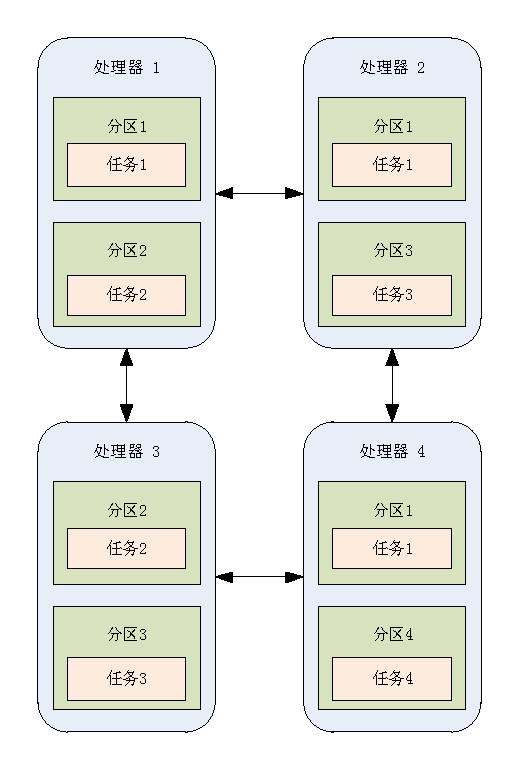
\includegraphics[height=60ex]{figure/DLS-task-partition-relation.pdf}\\
  \caption{处理器、分区和任务之间的关系}\label{DLS-fig-task-partition-relation}
\end{figure}

如在处理器 1 上,任务 $t_1$ 运行于分区1,我们在调度时为分区1分配的处理器时间分片的长度直接取决于其中运行的任务 $t_1$ 需要的运行时间,即 $t_1$ 的最坏运行时间 $C_1$。 这样,多核分区系统中对任务的调度,就转化为对分区的调度。由于每个任务的时间属性和任务之间的数据传输关系在调度前是已知的,我们就可以在系统运行前确定每个分区需要多少处理器时间,分别从哪个时刻开始到哪个时刻结束,这就是本文调度算法最后生成的针对每个处理器的任务调度表,同时也是每个处理器上的分区调度表。根据以上所述分区与任务间的一一对应关系,本文以下叙述中将不严格区分任务与分区的概念。

关于分区间的通信,如\ref{basic-partition-message}节所述,本文此处假定处于同一处理器的分区之间通信延迟可忽略,而不同处理器的分区间通信延迟与数据量和处理器之间的传输速率相关,在通信链路空闲的情况下,传递 M 的数据会造成 $M/s$ 的时间延迟。此外,本文将消息传递的距离也加入考虑:传递同样的数据量,随着消息跳数的增加,会稍稍增加传递延迟,使得跳数少的处理器结点被优先选择。
%\section{路由策略}
%
%在 \ref{basic-DAG-sch} 一节中介绍了 DAG 调度问题的几个分类,其中考虑处理器或核间消息路由的主要是 APN 类问题。在针对 APN 类问题的算法中,关注点主要集中于任务分配的顺序和任务向哪个处理器核心调度,至于消息路由则需要用户提供。因此在从DAG生成调度表时,首先也需要考虑了目标处理器平台的路由选择问题。%这里我们假定所有直接相连的核间通信的传输速率一致,也即相邻核间传输同样数据所花费的时间相同,这样,多核连接的拓扑结构就相当于一个边权值相等或无权的无向图。我们的路由选择策略总是选择路程最短,也即经过核数最少的路径。
%
%\subsection{静态路由}
%目标平台中,消息从一个核心发往另一个核心,对于静态路由来说,如果相同起点和终点,每次都选择同样的路径。最容易想到的,就是直接选择从起点到终点的最短路径。为简单起见,假定相邻(有链路直接相连的)处理器核心之间的数据传输速率都相同,那么目标处理器平台即成为一个无权无向连通图,处理器为顶点,链路为边,且所有边的权值都是1。在这个图上静态路由问题就化归为求解无权图任意顶点对之间的最短路径问题。假设图中顶点数为V,从图中一个顶点到达所有其他顶点的最短路径可以用一次广度优先顺序遍历得到,其复杂度为O$(V)$,那么求解所有顶点对之间最短路径的复杂度就是O$(V^2)$。
%
%静态路由的优点是路由信息可以事先计算,且算法实现方便。它的缺点在于不能根据消息在链路中的分布选择其他可以更早到达目标处理器核心的路径,这在非对称的处理器平台上有可能造成枢纽部分链路的消息过度密集而外围消息分布稀疏。
%
%\subsection{动态路由}
%
%动态路由在不同时刻从同一起点发往同一终点的消息可以选择不同的路径,其路径是在消息需要发送时才计算的,可以根据当时已调度消息在链路中的分布动态决定走哪条路径最快。这里的``快''指的是消息可以最早到达目标处理器核心,因此选择路径时势必要考虑不能覆盖所有可能链路上已分配的其他消息。
%
%即使是在无权连通图上,每次寻找从起点到终点的过程仍然是一个类似最短路问题中 Dijkstra 算法的过程,其复杂度为 O$(V\log{V})$,且在多次查找中仍需要针对同一起点和终点反复进行这一过程,大大提高了路由算法的开销,这是动态路由策略的一个劣势,开销较大、实现复杂。其优势是有可能找到更早到达的消息路由,使其后运行的任务有可能提前。但由于动态路由从路径上来说不一定是最短的,多次绕远路的消息路径有可能带来系统整体通信过大,也有造成原本可以更早调度的消息被多出来的通信开销给推后的结果。
%
%综合考虑以上两种路由策略的优劣,本文选择静态路由策略来实现算法。

% 路由算法描述:寻找最短路、生成下一跳矩阵





\section{任务分配}

本节首先假定任务调度是非抢占的,后面再对抢占式调度给出解决方案。

\subsection{任务排序与算法选择}

% DLS 最小松弛时间优先
% MH  最早时间限优先(未考虑不同任务可能由于约束条件 开始时间不同)
% 因此 DLS > MH

在\ref{basic-DAG-sch}一节中简要介绍了现有的几类 DAG 调度问题及其对应的算法。除了个别特殊条件下,DAG 调度本身几乎都是 NP 完全问题\upcite{DAGNP},在考虑数据通信的条件下,更进一步加大了问题的复杂性。文章 \cite{Comparison} 比较了解决 APN 问题的几种算法,并对不同条件下的调度结果做出了比较。% 描述优劣选择依据
%综合考虑调度优劣、算法本身的流程与我们这里所要解决问题的特殊性(虚拟结点的处理),我们选择 DLS 算法\upcite{DLS} 作为从 DAG 构建静态调度表的基础算法。

下面结合当前问题考虑相关算法的优劣。MH 算法\upcite{MHScheduling}根据 DAG 中每个结点的静态层数 (SBL) 属性排序,从大到小依次分配。由于 SBL 反映了该结点后面最少还有多少任务需要调度,SBL 越大说明任务需要越早完成。因此 MH 算法相当于单处理器实时调度中 EDF 算法的思想,时间限越早的任务具有更高的优先级。Dynamic Level Scheduling (DLS) 算法\upcite{DLS}则使用了一个动态层次 DL(Dynamic Level)作为排序标准。DL 是一个结点的 SBL 与它在一个处理器核心上的最早开始时间之差,具有最大 DL 的 (结点-核心) 对被挑选出来进行调度。这个值反映了该任务在满足时间限的前提下还有多大的调度空余度,相当于单处理器实时调度中最短空闲时间优先 (LLF) 算法的思想。

考虑在含有优先关系的多核调度环境下,不同任务由于制约条件不同,即使都处在可以运行的状态,能够开始的最早时间也可能不同。DLS 算法同时考虑了任务的开始与结束时间,而 MH 仅考虑任务的结束时间,这在所有就绪任务的最早开始时间不同的情况下未全面考虑所有因素。因此认为在当前问题的环境下,调度效果上 DLS 应当是优于 MH 算法的。

此外,如\ref{basic-DAG-sch}节所述,解决 DAG 调度 APN 问题的还有 BU 和 BSA 算法。这两类算法都是针对 DAG 调度问题的特点,首先将所有任务调度到枢轴处理器上去,再渐渐优化为更好的调度序列。但 DAG 调度问题不受虚拟任务结点的约束,在优化的过程中每一步都是一种可行调度方案,而在本文的 DAG 中,虚拟结点关于时间和连续调度的约束使得不能简单的将所有任务调度到一个处理器上,因此这两个算法都不太适合本文所述的情况。

综上所述,本文在此步骤中考虑使用 DLS 算法作为调度框架。

DLS 算法在调度的过程中,对就绪池中的每个结点,计算它们在所有处理器核心上的 DL,具有最大 DL 的 (结点- 核心) 对被挑选出来进行调度。其中在考虑各个任务于每个核心上的最早开始时间时,需要根据上一节提到的路由策略来决定,并同时记录下达到此开始时间时消息在链路上的调度信息。

% 为何不选用 BSA 。。。

\subsection{处理器排序}
\label{DLS-processor-sort}

% 来自 BSA 算法的思想,说明好处
% 最好有实验结果说明有必要对处理器核心排序

在将任务向处理器分配时,需要按一定顺序依次尝试将任务调度到各个处理器上。当某个任务在多个处理器上都具有相同的开始时间时,任务将被更优先于分配到排在前面的处理器上,因此,尝试分配的顺序对最终结果也会产生一定影响。如果排在前面的都是分布比较边缘的处理器,任务在目标平台上的分布也易分布于边缘,而边缘区处理器间连接数较少,造成通信路径比较长,整体通信开销变大。

我们借鉴 BSA 算法\upcite{BSA} 中任务分配顺序的思路,如果按照每个处理器的连接数从大到小排序,任务将更倾向于被分配到目标处理器平台的中枢地区,处理器间连接比较充分,之间的消息通信也比较通畅,使得整体系统通信开销减小。

\subsection{调度策略}

% 按时间段的查找方式分为
% 抢占、非抢占 两种

最终需要针对每个处理器核心,和每条链路都生成一个调度表。当需要将新任务加入某个处理器核心,或是将新消息加入对应链路上的消息调度表时,可以抢占或非抢占两种方式处理。如果是非抢占式调度,根据新添加任务所需的运行时间,需要在调度表中找到一块足够长的时间段将其分配给新任务;而对于抢占式调度,只需将任务按照时间限制尽早开始即可,如果一个时间段不够,则顺延至调度表的下一个时间段继续执行。

抢占与非抢占式调度在时间上的一大区别是,非抢占式调度根据任务的开始时间即可明确知道任务会在何时结束,而抢占式调度任务开始的早晚与任务结束的早晚并没有必然联系。这样,处理抢占式任务时,在以上 MDLS 算法中,在寻找 (任务-核心) 对时,需要将任务的最早开始时间改为考虑任务的最早完成时间,其他按原算法处理即可。

\section{虚拟结点}
\label{DLS-virtual-node}

DAG中的虚拟结点的处理需要考虑以下两个方面:
\begin{itemize}
  \item 它们不应当被分配到正常的处理器上去,否则将占用CPU 资源,延误普通任务的执行
  \item 它们和其他任务之间的通信数据不应当占用通信开销,因为所有数据也都是虚拟的,只用于表示先后依赖关系,并没有真正的数据流通。
\end{itemize}

可以在系统中加入一个虚拟分区专门用来分配虚拟任务。该分区与其他所有分区直接相连,且数据在与虚拟分区的链路传输不耗费时间。

在处理每个结点时,需要判断是否是虚拟结点,如果是则将其分配至虚拟处理器核心。根据 \ref{SDF-time-constraint} 一节所述,如果虚拟任务可以在虚拟处理器上连续分布,则所有任务的时间限都得到满足;否则,必有任务的时间限无法得到满足,调度失败。

\section{修改的DLS算法}
\subsection{算法流程}
综合考虑以上几节所讨论的问题,本文提出了修改的 DLS (Modified DLS, MDLS) 算法如算法 \ref{algo-MDLS} 所述。
\begin{algorithm}
  \caption{Modified DLS 算法}
  \label{algo-MDLS}
  \KwIn{包含虚拟结点的 DAG 任务图,目标处理器平台}
  \KwOut{任务和消息的静态调度表}
  向目标平台添加虚拟处理器\;
  将所有处理器按连接数降序排列\;
  计算 DAG 中所有结点的 SBL\;
  建立 ReadyTask 集合 S,并加入所有就绪结点\;
  \While{S 不空}{
      \uIf{S中有虚拟结点}{
          将结点尽可能早的调度至虚拟处理器\;
          \If{虚拟结点与前一个任务间有时间间隙}{
              无法得到有效调度\;
              算法结束\;
          }
      }\Else{
          考察 S 中所有任务与核组成的(任务-核)对,选择能够最早开始的任务,将其调度到对应的处理器上去\;
      }
  }
  更新 S 集合\;
\end{algorithm}

%\begin{Verbatim}[numbers=left,frame=single,xleftmargin=50pt]
%向目标平台添加虚拟处理器
%将所有处理器按连接数降序排列
%计算 DAG 中所有结点的 SBL
%建立 ReadyTask 集合 S,并加入所有就绪结点
%WHILE S不空 DO
%    IF S中有虚拟结点 THEN
%        将结点尽可能早的调度至虚拟处理器
%        IF 虚拟结点与前一个任务间有时间间隙 THEN
%            无法得到有效调度
%            算法结束
%        END IF
%    ELSE
%        考察S中所有任务与核组成的(任务-核)对,
%          选择能够最早开始的任务,将其调度到对
%          应的处理器上去
%    END IF
%    更新 S 集合
%END WHILE
%\end{Verbatim}

这样,即可得到目标平台每个处理器上的静态调度表,以及对应链路上的消息调度。

\subsection{复杂度分析}
\label{COSS-complexity}
假设 DAG 中结点个数为 $V_D$,目标平台处理器或核心数为 m。在上述算法过程中,对处理器按连接数降序排列的时间复杂度为 $O(m\log{}m)$,计算所有结点的 SBL 可由一遍深度优先遍历来完成,因此时间复杂度为 $O(V_D)$。

根据 \ref{basic-DLS-intro} 节的介绍可知,DLS 算法的时间复杂度为 $O({V_D}^{2}m f(m))$。与之相比,我们在 DLS 算法的循环内部添加了一个对虚拟结点的判断过程,该过程自身是$O(1)$的,而循环是对每个结点进行,因此与原 DLS 算法相比,总体多了一个 $O(V_D)$ 的过程。模型假设目标平台是静态路由,$f(m)=m$。

综上可知,对 MDLS 算法来说,总的复杂度为 $$O(m\log{}m)+O(V_D)+O({V_D}^{2}m^2)+O(V_D)=O({V_D}^{2}m^2)$$

再结合前两章中复杂度的分析,得到 COSS 算法总的复杂度为
$$O(V_G+E_G)+O(E_G+V_G+E_D+V_D)+O({V_D}^{2}m^2)=O(E_G+V_G+E_D+{V_D}^{2}m^2)$$
从 GSDF 到 DAG 的转换中,GSDF 中的每个结点都至少在 DAG 中出现一次,因此 $V_D\geqslant{}V_G$,对边来说也有类似关系 $E_D\geqslant{}E_G$,而 DAG 中边数最多为 $O({V_D}^2)$ 量级,因此上式可进一步化简为$$O({V_D}^{2}m^2)$$ 此即为 COSS 算法总的时间复杂度。

\section{本章小结}

本章设计了 COSS 算法的第三步,论述了从 DAG 求得静态调度表时所遇到目标平台抽象、任务分配和虚拟结点的处理等几个问题,针对每一问题分别讨论了可行方案及算法选择,最终提出了 MDLS 算法并给出了详细的描述。通过本章所述内容,COSS 算法主体部分结束,结合前两章,即可实现周期性任务集从时间、通信约束到目标平台的静态调度表。




% 算法实现 及 程序说明
% !Mode:: "TeX:UTF-8"
\chapter{程序设计与实现}
\label{chapter-program}

以上三章分别介绍了 COSS 算法的整个流程以及各部分要解决的问题,并分别讨论了针对各问题的解决方案。本章将依据以上思路,用模拟程序分模块实现整个算法。
%本章介绍实现算法模拟的程序功能、各部分所用的数据结构及实现中所考虑的一些细节。

\section{程序结构及功能}
\label{sec-prgraom-structure}
% 总体功能,包括需要哪些输入信息,程序分成哪几块,各完成什么任务,最后输出什么信息等
% 不需要具体格式及数据结构
由于算法的功能是将带有周期性时间约束和数据依赖约束的任务在满足以上约束的条件下调度到一定拓扑结构的多核处理器(或多处理器结构)上去,因此程序的输入输出信息主要也就围绕这些内容来设置。

\subsection{输入信息}
%输入内容包括每个任务的属性、任务之间的数据依赖关系、多核之间的拓扑连接情况以及数据传输率。其中任务的自身属性包括在单个处理器上最坏情况下的执行时间(Worst Case Execution Time, WCET)、任务是否是自依赖的,对与周期任务$t_i$,还包括它的周期长度$T_i$、 首次释放时间$O_i$、 相对时间限$D_i$等情况。任务的数据依赖关系$\textnormal{Dep}_{ij}=\{i,j,p_{ij},c_{ij},D_{ij}\}$ 是指两个任务$t_i$ 与$t_j$之间,$t_i$ 每执行一次,将向$t_j$ 发送$p_{ij}$ 个数据,而$t_j$ 每执行一次,将消耗从$t_i$ 发来的$c_{ij}$ 个数据。此外,$\textnormal{Dep}_{ij}$还包括初始状态下$t_i$ 与$t_j$ 之间已存在的可由$t_j$直接使用的数据量$D_{ij}$。最后,为得到较理想的调度结果,还需输入周期倍数参数$J$,表示程序在寻找可行调度时需在大周期中包含多少个最小周期。

程序的输入信息主要包括任务属性以及目标平台属性两方面内容。

\begin{enumerate}
  \item 任务属性
    \begin{itemize}
      \item 对每个任务 $t_i$,最坏情况下的执行时间$C_i$(Worst Case Execution Time, WCET)
      \item 任务是否是自依赖的(即是否必须串行执行)
      \item 对于周期性任务 $t_i$,包括周期长度$T_i$、 首次释放时间$O_i$、 相对时间限$D_i$ 等。
      \item 任务之间的依赖关系 $\textnormal{Dep}_{ij}=\{i,j,p_{ij},c_{ij},D_{ij}\}$。 指的是两个任务$t_i$ 与$t_j$之间,$t_i$ 每执行一次,将向$t_j$ 发送$p_{ij}$ 个数据,而$t_j$每执行一次,将消耗从$t_i$ 发来的$c_{ij}$ 个数据,以及初始状态下$t_i$ 与$t_j$ 之间已存在的可由$t_j$直接使用的数据量$D_{ij}$。
    \end{itemize}
  \item 目标平台属性
    \begin{itemize}
      \item 处理器的核数 M
      \item 两两核之间的连接情况,即连接矩阵
      \item 核间数据传输速率 s
    \end{itemize}
\end{enumerate}

此外,为得到更好的调度结果,有时还需要指定在一个调度大周期中包含多少个最小调度周期,即周期倍数 $J$。


\subsection{输出信息}

根据以上输入信息,如果程序针对目标平台能够找到可行调度,程序将输出两类调度列表:
\begin{enumerate}
  \item 针对每一个处理器核心生成任务调度表
  \item 针对每一条核间链路生成其上的消息调度表
\end{enumerate}

为补充输出信息的完整性,每个任务在周期内的多次执行在各个核上的空间与时间分布情况也将输出。此外,为反映算法过程,程序各步的中间结果信息也将会输出。

\subsection{程序结构}
从结构上来说,算法的模拟程序与 COSS 算法的整体流程相一致,主要分为数据输入、构建GSDF 图、从GSDF 构建DAG 最终由 DAG 生成调度表等几个模块。程序总的数据流程如图 \ref{PROG-fig-flow} 所示。

\begin{figure}[!hbt]
  \centering
  % Requires \usepackage{graphicx}
  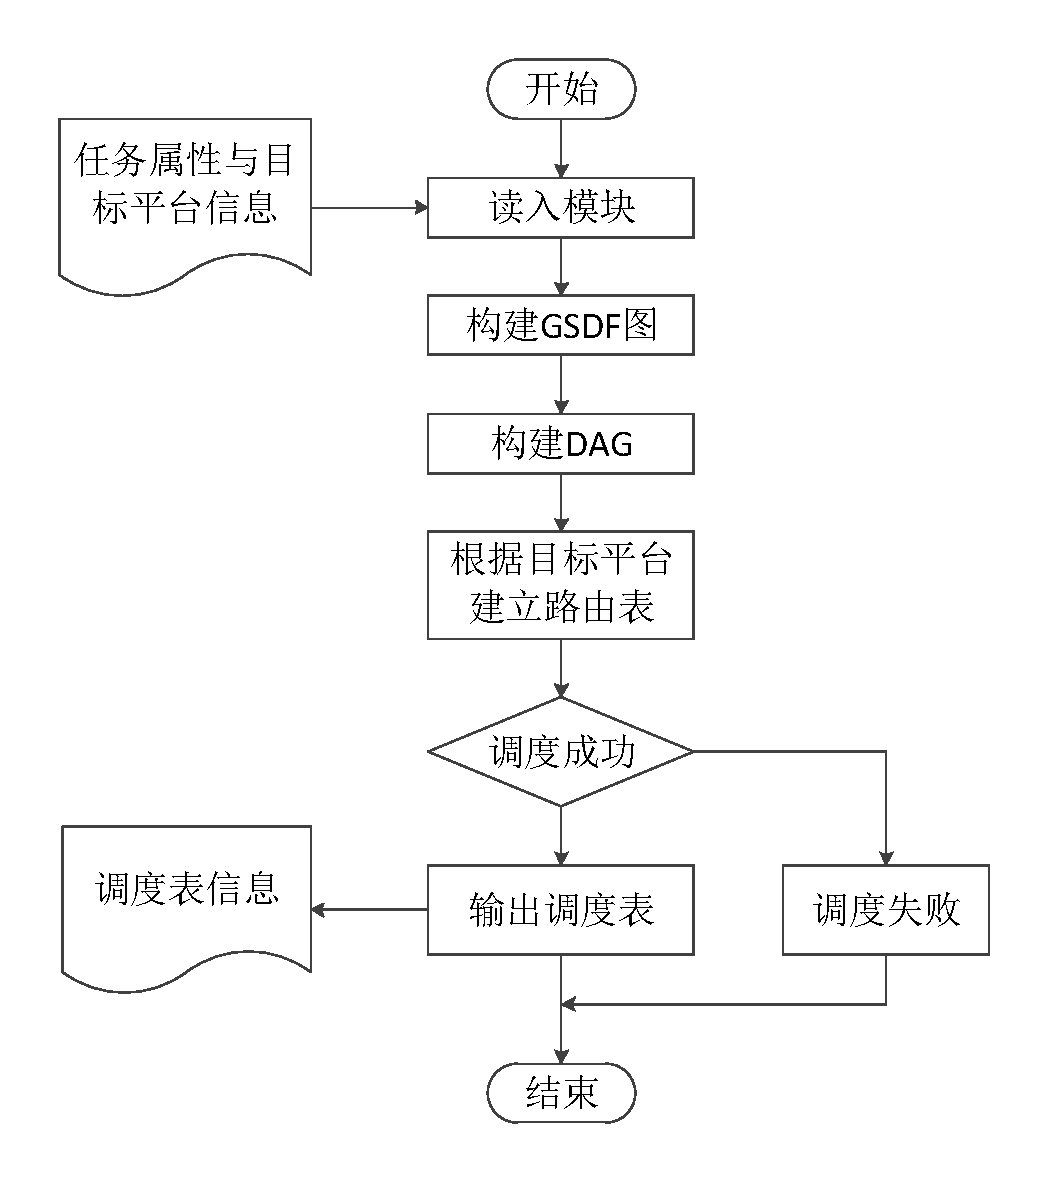
\includegraphics[height=55ex]{figure/PROG-flow.pdf}\\
  \caption{算法程序流程图}\label{PROG-fig-flow}
\end{figure}

根据以上流程,程序的功能模块划分如图\ref{PROG-fig-module}所示,各模块对应文件如表\ref{program-tab-file}所示。

\begin{figure}[!hbt]
  \centering
  % Requires \usepackage{graphicx}
  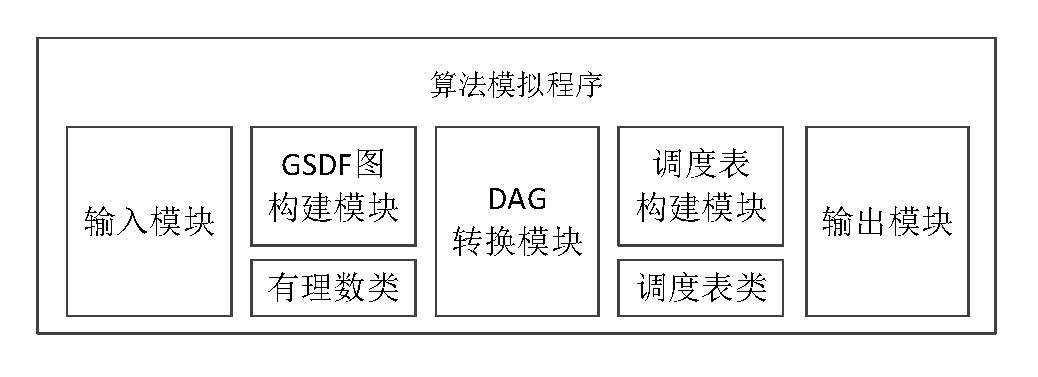
\includegraphics[height=20ex]{figure/PROG-module.pdf}\\
  \caption{模拟程序功能模块划分}\label{PROG-fig-module}
\end{figure}

{\renewcommand{\arraystretch}{1.5}
\begin{table}
  \centering
  \caption{程序文件描述}
  \label{program-tab-file}
  \begin{tabular}{|l|l|}
    \hline
    % after \\: \hline or \cline{col1-col2} \cline{col3-col4} ...
    Config.h & 设定任务数上限、调整浮点数计算精度等程序设置 \\
    input.cpp & 输入模块,读取输入数据并储存 \\
    Rational.h & 提供用于分数计算的类,解矩阵方程时用到 \\
    SDF.cpp & 从时间约束和数据约束构建 GSDF 图,并求解最小周期 \\
    DAG.cpp & ICS 算法从 GSDF 构建 DAG \\
    ScheduleList.h & 提供调度表类,方便对调度表的添加任务、查找空闲时间等操作 \\
    StaticSchedule.cpp & 消息路由、MDLS 算法从 DAG 求得调度表 \\
    main.cpp & 主程序\\
    \hline
  \end{tabular}
\end{table}
}

\section{详细设计}
每一模块的功能实现部分主要按照三、四、五章中的具体算法来完成。本节介绍在实现过程中存储结构的选择以及遇到的一些细节优化问题。

\subsection{数据输入}
\label{sec-data-structure}

每个任务的时间属性用一个 Task 结构体来表示,任务间通信关系用一个 Arc 结构体来表示,如表 \ref{program-tab-code-task} 所示。

{\renewcommand{\arraystretch}{1.5}
\begin{table}
  \caption{任务属性的结构体}
  \label{program-tab-code-task}
  \begin{lstlisting}[
      language={C},
      caption={}
      %label={program-code-task},
  ]
    // 时间约束
    struct Task
    {
        int wcet;        // 最坏运行时间
        int T;           // 周期
        int offset;      // 首次释放偏移
        int deadline;    // 时间限
        int selfdelay;   // 任务是否是自依赖的
                         // >0: 任务自依赖,运行时间需要数据通信
                         // =0: 任务自依赖,需要串行调度,但无数据通信
                         // <0: 任务不是自依赖,可以并行调度
    };

    // 数据依赖约束
    struct Arc
    {
        int src;         // 源任务结点
        int produce;     // 每次执行产生的数据
        int snk;         // 目标任务结点
        int consume;     // 每次执行消耗的数据
        int delay;       // 初始时弧上的 Delay
    };
  \end{lstlisting}
\end{table}
}

输入任务的信息和通信关系分别用一个数组 tasks 和 arcs 表示。

\subsection{GSDF图数据结构}

按第\ref{chapter-SDF}章所述算法可构建 GSDF 图。常用的图存储模式有邻接矩阵与邻接表,一般邻接矩阵适合于边稠密的图,而 GSDF 图中边数主要与任务间的数据依赖关系数有关,全部任务两两之间都有数据依赖的情况较少见,因此程序选择邻接表存储方式,空间占用与边的多少相关。GSDF 图的存储结构如图 \ref{PROG-fig-GSDF-structure} 所示。
为了方便遍历,我们不仅将某结点的出弧存储在此结点对应链表中,该结点的入弧同样也存储进来,这样从一个结点出发即可访问所有和它有数据依赖关系的全部结点,为求解拓扑矩阵提供方便。此外,在存储结构中将 GSDF 的反向弧也保存在邻接表中,这样,在修改某条弧上的缓冲区数值时,对应反向弧也方便一起修改,免去查找过程。

\begin{figure}[!hbt]
  \centering
  % Requires \usepackage{graphicx}
  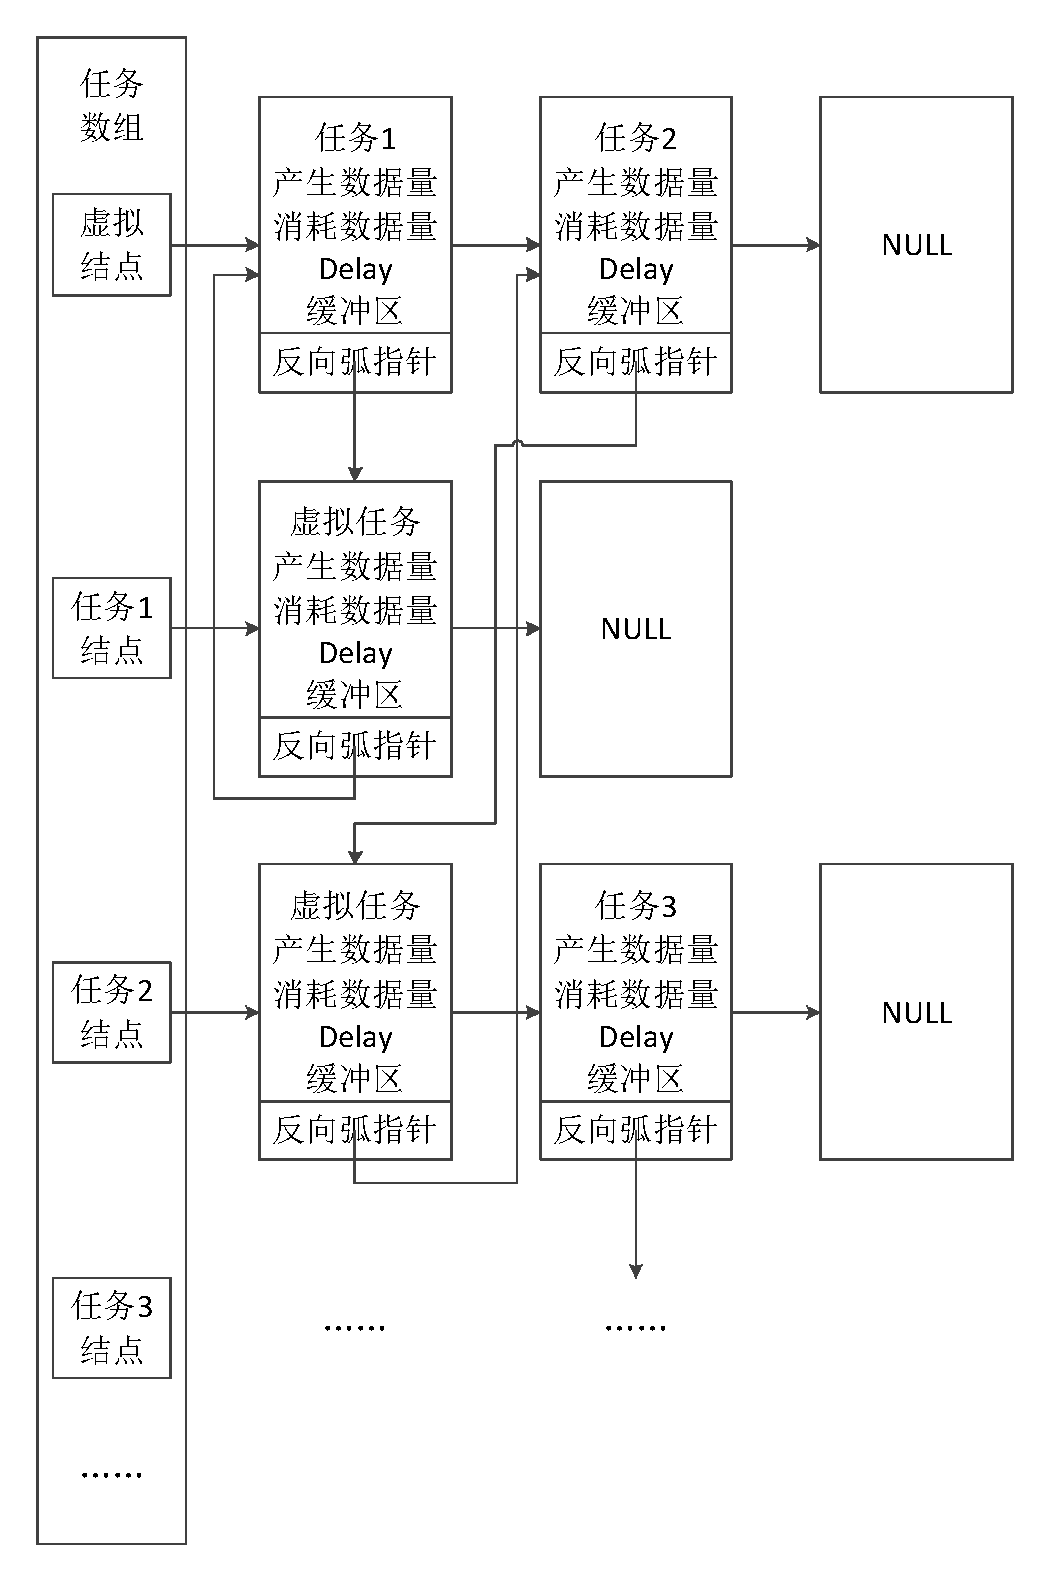
\includegraphics[height=63ex]{figure/PROG-fig-GSDF-structure.pdf}\\
  \caption{GSDF 数据结构图}\label{PROG-fig-GSDF-structure}
\end{figure}


%边的数据结构如代码 \ref{program-code-GSDF} 所述
%
%\begin{lstlisting}[
%    language={C},
%    caption={GSDF 的数据结构},
%    label={program-code-GSDF},
%]
%struct AdjNode
%{
%    int toTaskIdx;
%    int produce;    // < 0 on revarcs in sdf
%    int consume;    // < 0 on revarcs in sdf
%    int delay;      // always 0 on revarcs in sdf
%    int buffer;     // always 0 on revarcs in sdf
%    AdjNode *revarc;
%};
%
%list<AdjNode> sdf[MAXTASKNUM];    // sdf[0] is the virtual node,
%                                  // sdf[1]~sdf[N] are task nodes.
%\end{lstlisting}

在求解拓扑矩阵时,考虑到矩阵的特殊性质:每行仅有两个非零值,且一正一负。由以上特性可知向量解中两两分量间的比例关系,直接在 GSDF 图中采用一次深度优先遍历即可求得所有分量间的比例关系,取其最小公倍数,即容易得出拓扑矩阵的最小整数解向量,大幅降低了解方程的复杂度。为了求解拓扑矩阵,本模块还对有理数的运算做了封装,用于对分数运算的精确处理,以及最后求解分数的公倍数提供方便。

%\subsection{从GSDF到DAG}
% 矩阵解法
% 等等
%\emph{TODO: 矩阵解法}


%\emph{TODO: 结点间数据传输的处理}
%关于上一章提到的处理周期内与周期间数据传输的问题,由于细节处理方面判断分支很多,代码量较大,请具体参阅程序源码对应部分。

\subsection{目标平台的下一跳矩阵}
% 所有点对间最短路
%\emph{TODO: 所有点对间无权图最短路径}
按上一章所述,处理器间消息传递的路由选择按最少跳数进行。模拟程序为输入方便,仅输入了目标处理器平台的连接矩阵,因此程序在确定消息路径之前需要计算核之间的无权最短路径,并得到目标平台的下一跳矩阵。
模拟程序中由处理器之间连接关系的邻接矩阵直接构建所有核之间的下一跳矩阵,采用层级广度优先遍历的顺序,在找到最短消息路径的同时,也将下一跳信息储存下来,形成下一跳矩阵。


%在进行 DLS 算法之前,首先求出目标平台所有核间的最短通路,并求出指向最短通路的下一跳矩阵。
% 给出求下一跳矩阵的算法描述

\subsection{用MDLS方法构建静态调度表}

在调度表构建模块中,为方便对调度表的操作,模拟程序设计了 ScheduleList 类,将与调度表的有关操作封装起来,专用来处理与调度表相关的任务。其类声明如表 \ref{program-code-SchList} 所示。

{\renewcommand{\arraystretch}{1.5}
\begin{table}
  \caption{调度表类}
  \label{program-code-SchList}
    \begin{lstlisting}[
        language={C},
        caption={}
    ]
    template<class DataType>
    class ScheduleList
    {
    public:
        double lastSlot() const;
        double findSlot(double stTime, double span) const;
        bool insertWork(double time, double span, const DataType &data);

        // 保存当前状态
        void save();
        // 回退到上一次保存的状态
        void drawback();

        void print(FILE *fp, char *preStr) const;
    };
    \end{lstlisting}
  \end{table}
}

在实现 MDLS 算法中,需要频繁操作对应各个处理器和链路上的调度表,因此有必要将其独立出来作为一个类专门处理关于调度表的各项操作,例如添加一个新任务安排,查找满足一定条件的时间空隙等等。特别的,为了处理 MDLS 中因尝试调度计算最早开始时间而产生的回溯情况,在此类中添加保存状态和恢复保存的状态接口,为程序编排和代码逻辑清晰度都带来很大好处。ScheduleList 类的主要接口功能如表 \ref{program-tab-SchList-mem} 所示。其中 drawback() 在恢复时实际使用 swap 方法,只交换指针不交换调度表内容即可将调度表状态还原,减少了数据复制的开销。

{\renewcommand{\arraystretch}{1.5}
\begin{table}
  \centering
  \caption{调度表类的接口功能说明}
  \label{program-tab-SchList-mem}
  \begin{tabular}{l|l}
    \hline
    lastSlot() & 返回最后一个空闲时间段的起始时间 \\
    findSlot() & 从给定的时间开始向后,找到一个大于给定值的空闲时间段,返回开始时间 \\
    insertWork() & 想调度表中添加新的任务安排\\
    \hline
    save() & 为方便 MDLS 调度中储存临时状态以便调度不成功时回溯,此函数可保存调\\
           & 度表当前状态 \\
    drawback() & 将调度表恢复到上一次保存的状态。\\
    \hline
    print() & 打印调度表\\
    \hline
  \end{tabular}
\end{table}
}


\section{本章小结}

本章设计并实现了COSS算法的模拟程序。文中首先根据算法流程对模拟程序的功能模块做了划分,并设计了程序的输入输出文件格式。其次,针对程序实现过程中相关信息存储时数据结构的选择等问题提出了代码优化方案,并给出了实现方式。最后,本章对调度表构建模块中对调度表所需的一些具体操作进行了封装,并提出了采用 swap 方式优化状态保存及返回状态两个操作。



% 例子分析
% !Mode:: "TeX:UTF-8"

\chapter{程序结果分析}

%\emph{TODO}: 按通信量与计算时间的比例大小分类、按拓扑结构分类(消息拥塞)、按时间与数据依赖的相对多少分类

%本节通过几个例子分别验证 COSS 算法的流程、处理器排序优化、目标平台的连接对调度结果的影响等,分析几种不同类型任务集的调度结果。
本节通过例子来具体演示 COSS 算法的流程,并分析调度结果在时间约束、数据约束以及子依赖约束等方面的正确性。
\section{算法流程示例}

%\emph{TODO: 给出一个具体例子的输入输出,并结合例子分析说明}

例如有周期任务 A 和 B,运行时间分别为 $C_1=1$ 和 $C_2=2$,周期性时间属性分别为:
\begin{gather*}
  T_A=2, O_A=0, D_A=2 \\
  T_B=3, O_B=0, D_B=3
\end{gather*}
且 A、B 任务之间具有如图 \ref{program-fig-sample-SDF} 所示的通信关系。即任务 A 每次执行向 B 发送 2 个数据,任务 B 每次执行需要消耗由 A 发来的 3 个数据,初始时 B 有 3 个数据可用。由此通信关系造成的数据依赖约束如图中右侧关系所示,任务 B 的第 1 次执行需要受 A 第 1 次运行结束的制约,B 的第 2 次执行受到 A 第 2 次运行结束的制约。

\begin{figure}[!hbt]
  \centering
  % Requires \usepackage{graphicx}
  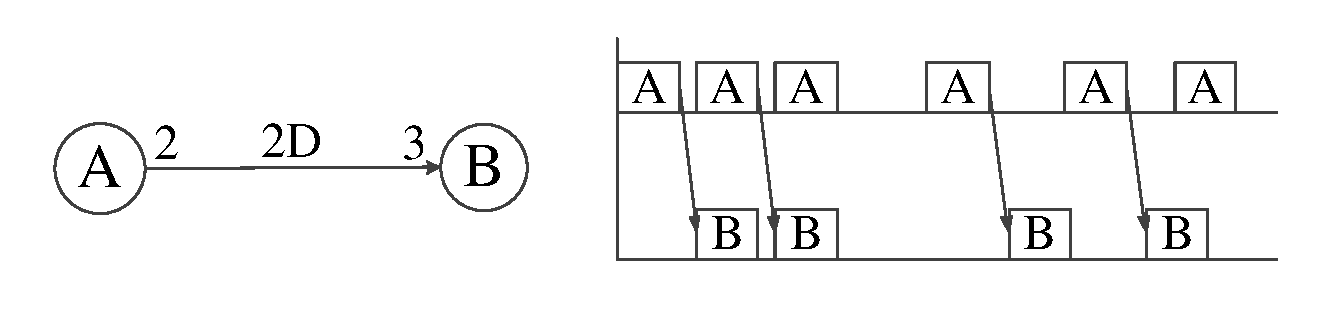
\includegraphics[height=12ex]{figure/program-sample-SDF.pdf}\\
  \caption{A、B 任务之间的通信关系}\label{program-fig-sample-SDF}
\end{figure}

假设将 A、B 调度到由两个处理器组成的目标平台,其连接矩阵为
$$C=\begin{bmatrix}-1 & 1 \\ 1 & -1\end{bmatrix}$$
处理器间通信速率 $s=10$,表示每单位时间从一个处理器向另一个处理器可发送 10 个单位的数据。根据附录所述输入格式,将其整理为如下输入文件:%如表\ref{program-tab-input} 所示。
%{\renewcommand{\arraystretch}{1.5}
%\begin{table}
%  \centering
%  \caption{输入文件示例}
%  \label{program-tab-input}
%  \begin{tabular}{r|l|l}
%    \hline
%      行号 & 文件内容 & 说明\\
%    \hline
%      1 & 2 & 任务数\\
%      2 & 1 2 0 2 -1 & 任务 A 的时间属性\\
%      3 & 2 3 0 3 -1 & 任务 B 的时间属性\\
%      4 & 1 & 任务间数据依赖的个数\\
%      5 & 1 2 2 3 2 & 数据依赖关系\\
%      6 & 1 & 周期倍数\\
%      7 & 2 & 处理器个数\\
%      8 & 10 & 消息传输速率\\
%      9 & 1 & 连接数\\
%      10 & 1 2 & 处理器间连接\\
%    \hline
%  \end{tabular}
%\end{table}
%}
\begin{Verbatim}[numbers=left,frame=single,xleftmargin=50pt,
samepage=true,fontsize=\small,baselinestretch=1.2]
2
1 2 0 2 -1
2 3 0 3 -1
1
1 2 2 3 2
1
2
10
1
1 2
\end{Verbatim}

其中第一行数字 2 表示任务个数,下面 2 行分别表示任务 A 和 B 的时间约束,每行最后的数字 -1 表示该任务不是自依赖的,即没有数据需要在同任务的相邻两次执行之间传递。第四行的数字 1 表示任务间通信关系的个数,下面 1 行表示任务 A、B 之间的具体通信关系。第六行数字 1 表示周期倍数,第七行数字 2 表示目标平台的处理器个数,下面的数字 10 表示处理器之间的通信速率。第九行数字 1 表示处理器之间的连接数,最后 1 行表示哪两个编号的处理器之间有链路相连。

模拟程序按以上信息调度,输出内容分为求解拓扑矩阵、DAG、生成的静态路由表、调度表等几部分。

程序输出拓扑矩阵为:
\begin{equation*}
  \Gamma=\begin{bmatrix}
    1 & -2 & 0 \\
    1 & 0 & -3 \\
    -1 & 2 & 0 \\
    0 & 2 & -3 \\
    -1 & 0 & 3
  \end{bmatrix}
\end{equation*}

由输入任务的时间属性以及任务间的通信关系,用第\ref{chapter-SDF}章介绍的方法,可以构建 GSDF 如图\ref{EXP-fig-GSDF} 所示。考虑到矩阵第1列对应虚拟结点V,第2 列对应任务结点A,第3列对应任务结点B,矩阵的每一行分别对应从 V 到 A 的弧、从 V 到 B 的弧、从 A 到 B 的弧、从 A 到 V 的弧以及从 B 到 V 的弧。可以看到,以上拓扑矩阵与任务 A、B 构建的 GSDF 相符。

\begin{figure}[!hbt]
  \centering
  % Requires \usepackage{graphicx}
  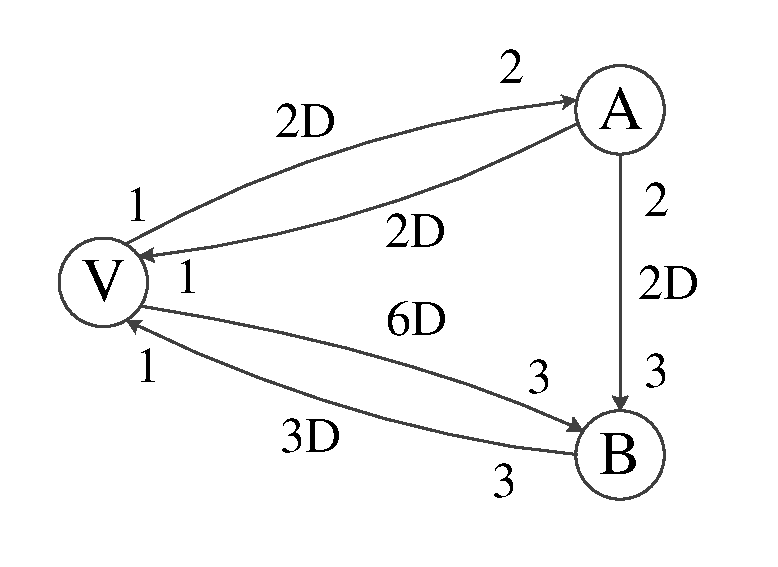
\includegraphics[height=20ex]{figure/EXP-GSDF.pdf}\\
  \caption{A、B 任务构建的 GSDF}\label{EXP-fig-GSDF}
\end{figure}

程序求出以上拓扑矩阵零空间向量的最小整数解为

\begin{equation*}
  q=\begin{bmatrix}
    6 \\
    3 \\
    2
  \end{bmatrix}
\end{equation*}

由以上 GSDF 和 q 构建 DAG,程序输出如下:
\begin{Verbatim}[numbers=left,frame=single,xleftmargin=50pt,
samepage=true,fontsize=\small,baselinestretch=1.2]
======== DAG ========
Task 1:
  (1, 0): (0 2) 0; (2 0) 1; (2 1) 1;
  (1, 1): (0 4) 0; (2 1) 2;
  (1, 2): NP (0 0) 0; NP (0 1) 0; NP (2 0) 2;

Task 2:
  (2, 0): (0 3) 0;
  (2, 1): NP (0 0) 0; NP (0 1) 0; NP (0 2) 0;
\end{Verbatim}

其中 Task 0 表示虚拟任务 V,Task 1 表示任务 A,Task 2 表示任务 B。 任务 i 的第 j 次运行以一对整数 (i, j) 表示,每一行对应从 (i, j) 发出的,向其他任务结点发送的通信信息以及传输数据量。如 (1, 0): (2 0) 1 表示任务 1 的首次运行会向任务 2 的首次运行发送 1 的数据量。如果数据量为 0,表明任务间仅有时间上的制约关系,没有实际的数据通信,这种情况多发生于周期性任务与虚拟任务结点之间。
输出信息中的 NP 表示跨周期结点间的消息传输目标与数据传输量。以上一个调度周期的 DAG 可以表示为图 \ref{EXP-fig-DAG} 所示,其中 $A_2$ 与 $B_0$ 结点间表示跨周期结点间的消息。 图中弧上的数字表示结点间的通信数据量,结点旁的数字为该结点的 SBL 值。从图中可以看出,任务间的通信消息(包括调度周期内和周期间)一共有 4 条。

\begin{figure}[!hbt]
  \centering
  % Requires \usepackage{graphicx}
  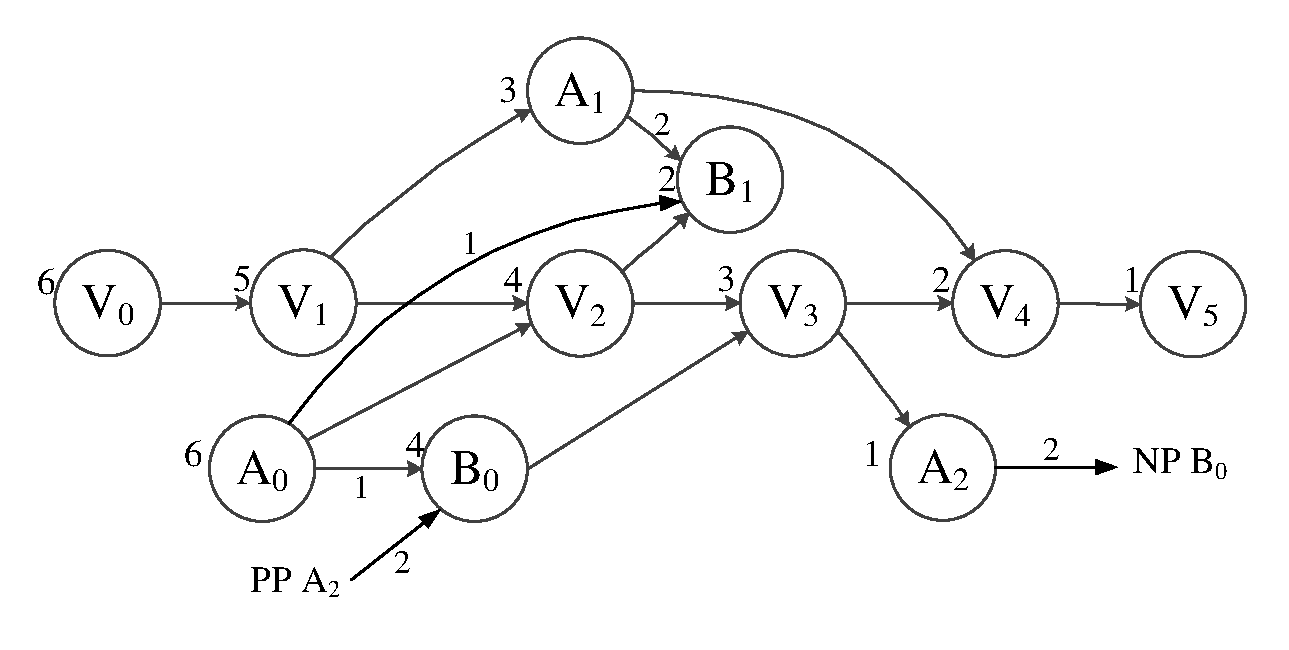
\includegraphics[height=28ex]{figure/EXP-DAG.pdf}\\
  \caption{A、B 任务构建的 DAG}\label{EXP-fig-DAG}
\end{figure}


目标平台是仅有两个核心的处理器,因此路由表非常简单,链路也只有一条,程序输出的下一跳矩阵为
$$H=\begin{bmatrix}-1 & 2\\ 1 & -1\end{bmatrix}$$
最终根据以上 DAG
得到的调度结果为:
\begin{Verbatim}[numbers=left,frame=single,xleftmargin=50pt,
samepage=true,fontsize=\small,baselinestretch=1.2]
===== Schedules =====
Processor 1:
     0.00 -->  1.00: Task (1 0), time 1
     1.00 -->  3.00: Task (2 0), time 2
     4.00 -->  5.00: Task (1 2), time 1

Processor 2:
     2.00 -->  3.00: Task (1 1), time 1
     3.00 -->  5.00: Task (2 1), time 2

Link 1 --- 2:
     1.00 -->  1.10: Task (1 0) --> (2 1), Processor 1 --> 2, data 1

  ---- Task ----
Task 1:
    (1 0): [Processor   1] time  0.00 -->  1.00
    (1 1): [Processor   2] time  2.00 -->  3.00
    (1 2): [Processor   1] time  4.00 -->  5.00

Task 2:
    (2 0): [Processor   1] time  1.00 -->  3.00
    (2 1): [Processor   2] time  3.00 -->  5.00
\end{Verbatim}
由调度结果可以看出,Task 1 的 3 次运行分别在 [0.0, 2.0)、[2.0, 4.0)、[4.0, 6.0) 的时间范围内,Task 2 的 2 次运行分别在 [0.0, 3.0)、[3.0, 6.0)] 的时间范围内,他们的周期性时间约束得到了保证。通信约束方面,Task 2 的第一次执行 (2 0) 是在 [1.0, 3.0) 时段,在 Task 1 的第一次运行 (1 0) 结束后,两者位于同一处理器核心,因此链路上没有这条消息调度。Task 2 的第 2 次执行 (2 1) 是 [3.0, 5.0) 时段,也在 Task 1 的第 2 次执行 ([2, 3] 时段) 结束后,因此周期内的优先关系制约得到了满足,且这两次执行均处于同一处理器,因此也不需在链路上进行消息调度。而 Task 2 的第 2 次执行 (2 1) 需要从 Task 1 第 1 次执行 (1 0) 得到数据,因此在链路上有这条消息的调度。最后,任务 1 的第三次执行 (1 2) 需要向下一周期任务 2 的第一次执行 (2 0) 发送 2 数据的消息,而从调度表可以看出这两者都位于处理器1,因此链路上也无需对这条消息调度。以上调度如图 \ref{EXP-fig-sch1} 所示。

\begin{figure}[!hbt]
  \centering
  % Requires \usepackage{graphicx}
  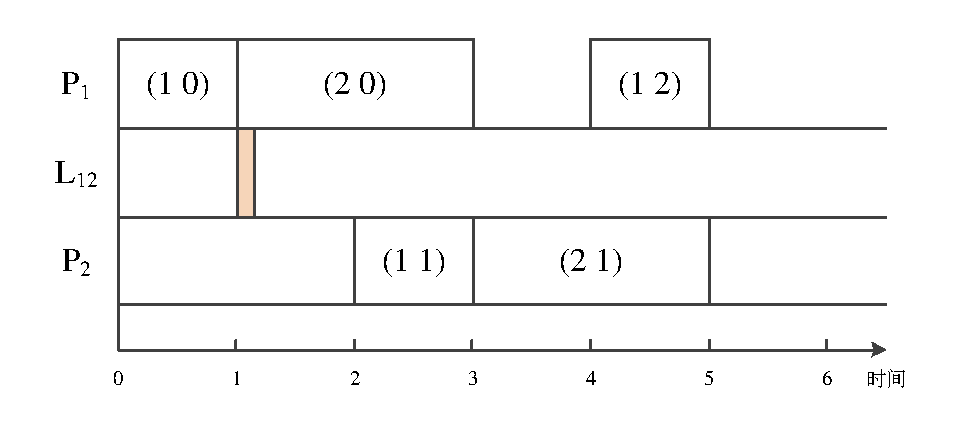
\includegraphics[height=25ex]{figure/EXAMP-sch1.pdf}\\
  \caption{简单例子的调度图}\label{EXP-fig-sch1}
\end{figure}

经过以上分析可以看到,两个任务均在时间限制约束的范围内,且满足了 A、B 之间数据通信的关系。其跨核的消息调度也得以体现。

%\section{处理器排序对调度结果的影响}
%在第 \refl{DLS-processor-sort} 节我们讨论了通过对处理器排序来优化调度结果,使任务更倾向于分配在连接数较多的处理器上,

\section{任务自依赖约束的验证}

为了验证任务自依赖属性对调度结果的影响,下面考虑由六个任务组成的任务集,其任务的时间约束如表\ref{EXP-table-6task-time} 所示,其任务间的数据通信关系如图\ref{EXP-fig-6task-SDF}所示。可以看到六个任务分成了两组各自连通的 SDF 图,其调度关系通过任务的时间约束联系起来。
{\renewcommand{\arraystretch}{1.5}
\begin{table}
  \centering
  \caption{6个任务的时间约束}
  \label{EXP-table-6task-time}
  \begin{tabular}{|c|c|c|c|c|c|}
    \hline
    % after \\: \hline or \cline{col1-col2} \cline{col3-col4} ...
    任务 & 最坏执行时间$C_i$ & 周期$T_i$ & 偏移$O_i$ & 时间限$D_i$ & 自依赖\\
    \hline
    1 & 25 & 60 & 0 & 60 & 否\\
    2 & 30 & 0 & 0 & 0 & 否\\
    3 & 20 & 45 & 0 & 45 & 否\\
    4 & 15 & 0 & 0 & 0 & 否\\
    5 & 10 & 60 & 20 & 30 & 否\\
    6 & 30 & 0 & 0 & 0 & 否\\
    \hline
  \end{tabular}
\end{table}
}
\begin{figure}[!hbt]
  \centering
  % Requires \usepackage{graphicx}
  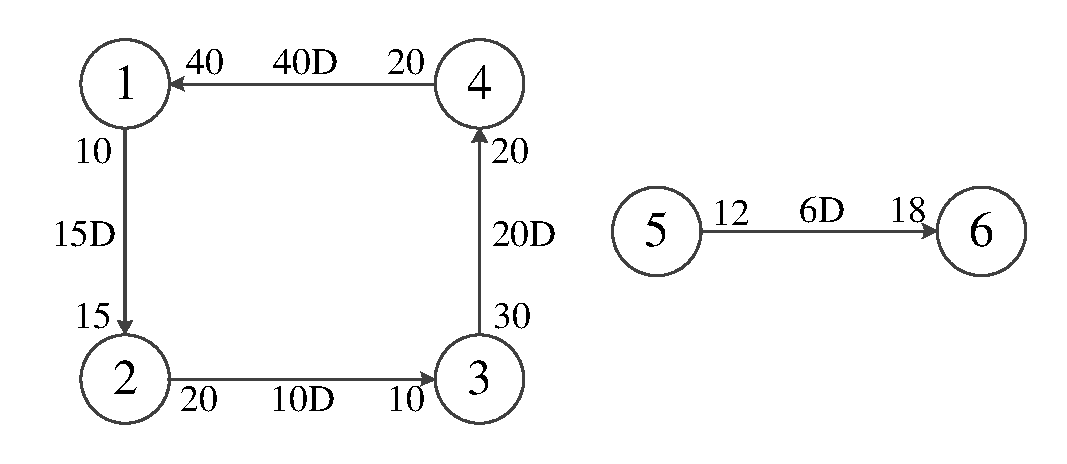
\includegraphics[height=24ex]{figure/EXP-6task-SDF.pdf}\\
  \caption{6个任务的 SDF 图}\label{EXP-fig-6task-SDF}
\end{figure}

调度的目标平台由三个处理器组成,其中处理器1和2相连,2和3相连。另外,为了明确反应数据通信延迟对调度所造成的影响,处理器之间的数据传输速率设为每单位时间1 个数据。我们调用算法模拟程序,可以得到如图\ref{EXP-fig-6task-sched1} 所示的调度结果。由于在表\ref{EXP-table-6task-time} 中所有任务都不是自依赖的,即同一任务在周期内的多次执行不必是串行的,可以看到以下调度图中任务4的几次运行中 (4,0) 和 (4,1) 在时间上有相互重叠的部分,(4,4) 和 (4,5) 也有重叠的部分。如果我们改变任务参数,将任务 4 改为自依赖的,其相邻两次执行之间需要传递10单位的数据,则调度图成为图\ref{EXP-fig-6task-sched2} 所示的结果。
\begin{figure}[!hbt]
  \centering
  % Requires \usepackage{graphicx}
  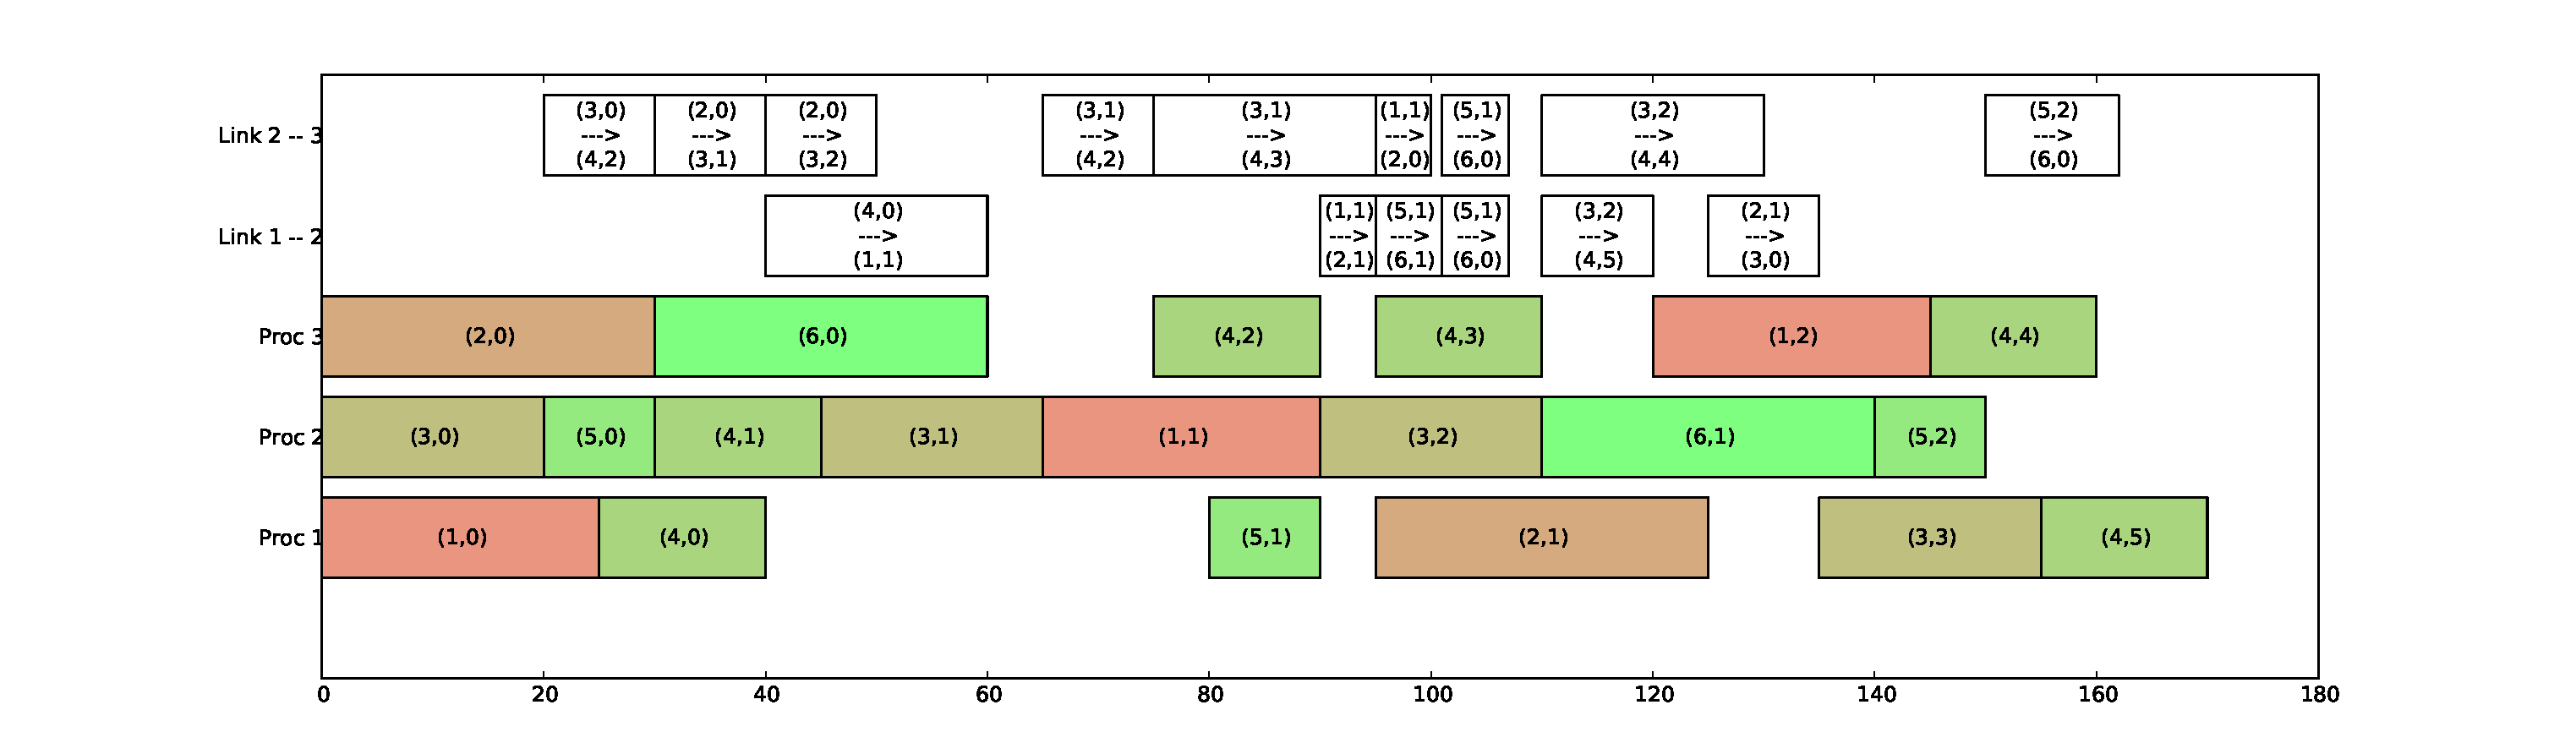
\includegraphics[width=40em]{figure/EXP-6task-sched1.pdf}\\
  \caption{6 个任务的调度表}\label{EXP-fig-6task-sched1}
\end{figure}
\begin{figure}[!htb]
  \centering
  % Requires \usepackage{graphicx}
  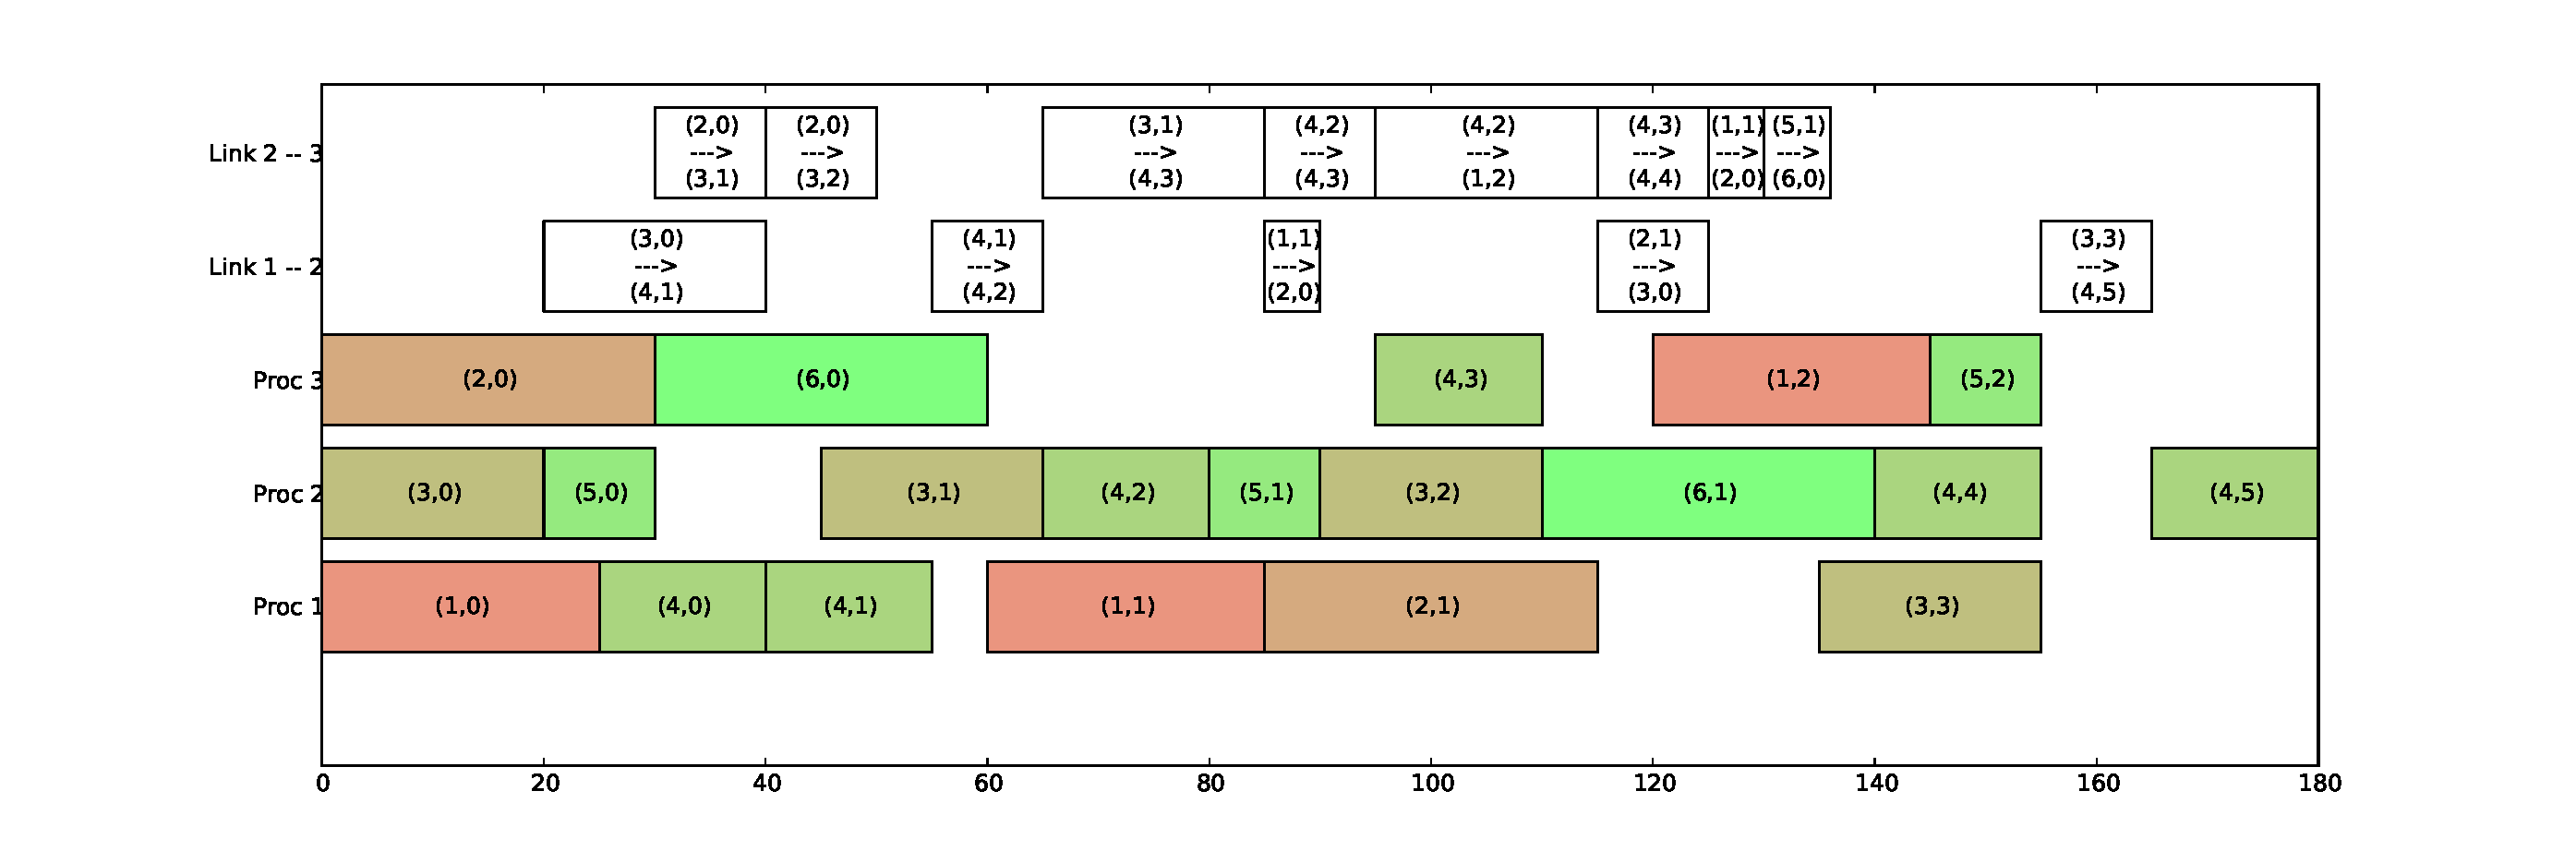
\includegraphics[width=40em]{figure/EXP-6task-sched2.pdf}\\
  \caption{添加自依赖后 6 个任务的调度表}\label{EXP-fig-6task-sched2}
\end{figure}

从图\ref{EXP-fig-6task-sched2}中可以看到任务4的执行区间 (4,0)、(4,1)、...、(4,5) 在时间上已不再有重叠,全部变为了串行执行,执行之间的通信开销也被考虑进了链路上的消息调度中。

\section{处理器排序对调度结果的影响}
下面我们来考察处理器排序对调度结果所造成的影响。在以上六个任务组成的任务集中,再添加三个任务,得到如表\ref{EXP-table-9task-time}所示的任务集,任务间的通信关系如图\ref{EXP-fig-9task-SDF}所示。其中 1---4 号任务和 7---9 号任务分别组成一个循环的通信关系,5号和6号任务组成单向的通信关系。
{\renewcommand{\arraystretch}{1.5}
\begin{table}
  \centering
  \caption{9个任务的时间约束}
  \label{EXP-table-9task-time}
  \begin{tabular}{|c|c|c|c|c|c|}
    \hline
    % after \\: \hline or \cline{col1-col2} \cline{col3-col4} ...
    任务 & 最坏执行时间$C_i$ & 周期$T_i$ & 偏移$O_i$ & 时间限$D_i$ & 自依赖\\
    \hline
    1 & 25 & 60 & 0 & 60 & 否\\
    2 & 30 & 0 & 0 & 0 & 否\\
    3 & 20 & 45 & 0 & 45 & 否\\
    4 & 15 & 0 & 0 & 0 & 否\\
    5 & 10 & 60 & 20 & 30 & 否\\
    6 & 30 & 0 & 0 & 0 & 否\\
    7 & 20 & 36 & 0 & 36 & 否\\
    8 & 30 & 0 & 0 & 0 & 否\\
    9 & 20 & 0 & 0 & 0 & 否\\
    \hline
  \end{tabular}
\end{table}
}
\begin{figure}[!hbt]
  \centering
  % Requires \usepackage{graphicx}
  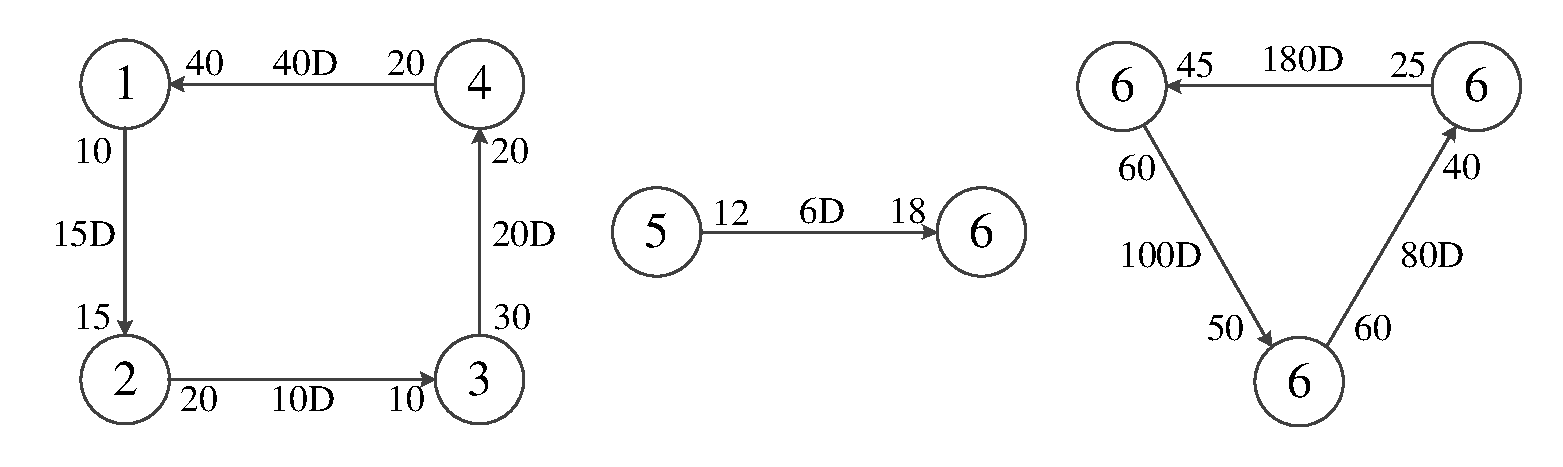
\includegraphics[height=24ex]{figure/EXP-9task-SDF.pdf}\\
  \caption{9个任务的 SDF 图}\label{EXP-fig-9task-SDF}
\end{figure}

在由7个处理器组成的目标平台上,处理器之间的拓扑连接如图\ref{EXP-fig-7p-link}所示。7 号处理器处于中枢位置,与其余 6 个处理器都相连,此外 1 和 2 号以及 4 号和 5 号处理器也分别相连。处理器之间的数据传输速率依然设为 1。
\begin{figure}[!hbt]
  \centering
  % Requires \usepackage{graphicx}
  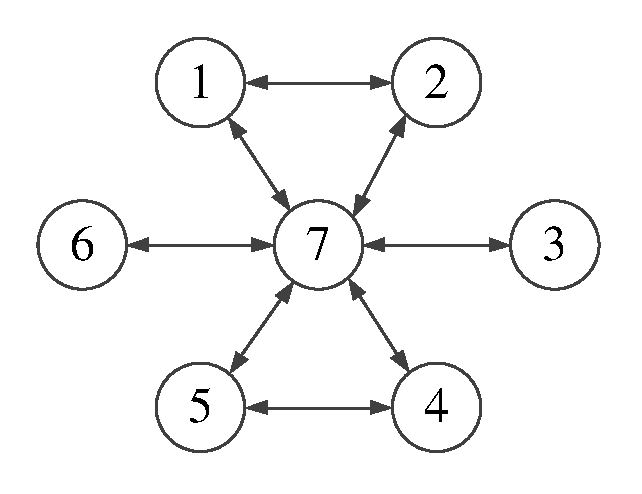
\includegraphics[height=20ex]{figure/EXP-7p-link.pdf}\\
  \caption{目标平台7个处理器间的拓扑连接}\label{EXP-fig-7p-link}
\end{figure}

将以上信息构建输入调度算法模拟程序,可以得到如图\ref{EXP-fig-9task}所示的调度表,说明此任务集可以调度。从以上处理器的托普连接可以看出,7号处理器的连接数是 6 为最多,其次是 1、2、4、5 号处理器,连接数均为 2,最后是 3 和 6 号处理器,连接数只有 1。按照处理器排序的情况下,程序的搜索顺序即为 7、1、2、4、5、3、6,当任务的开始时间相同时,且消息传递跳数相同的情况下,任务倾向于排布在靠前的处理器上,处理器之间连接通畅,易于消息调度。
\begin{figure}[!hbt]
  \centering
  % Requires \usepackage{graphicx}
  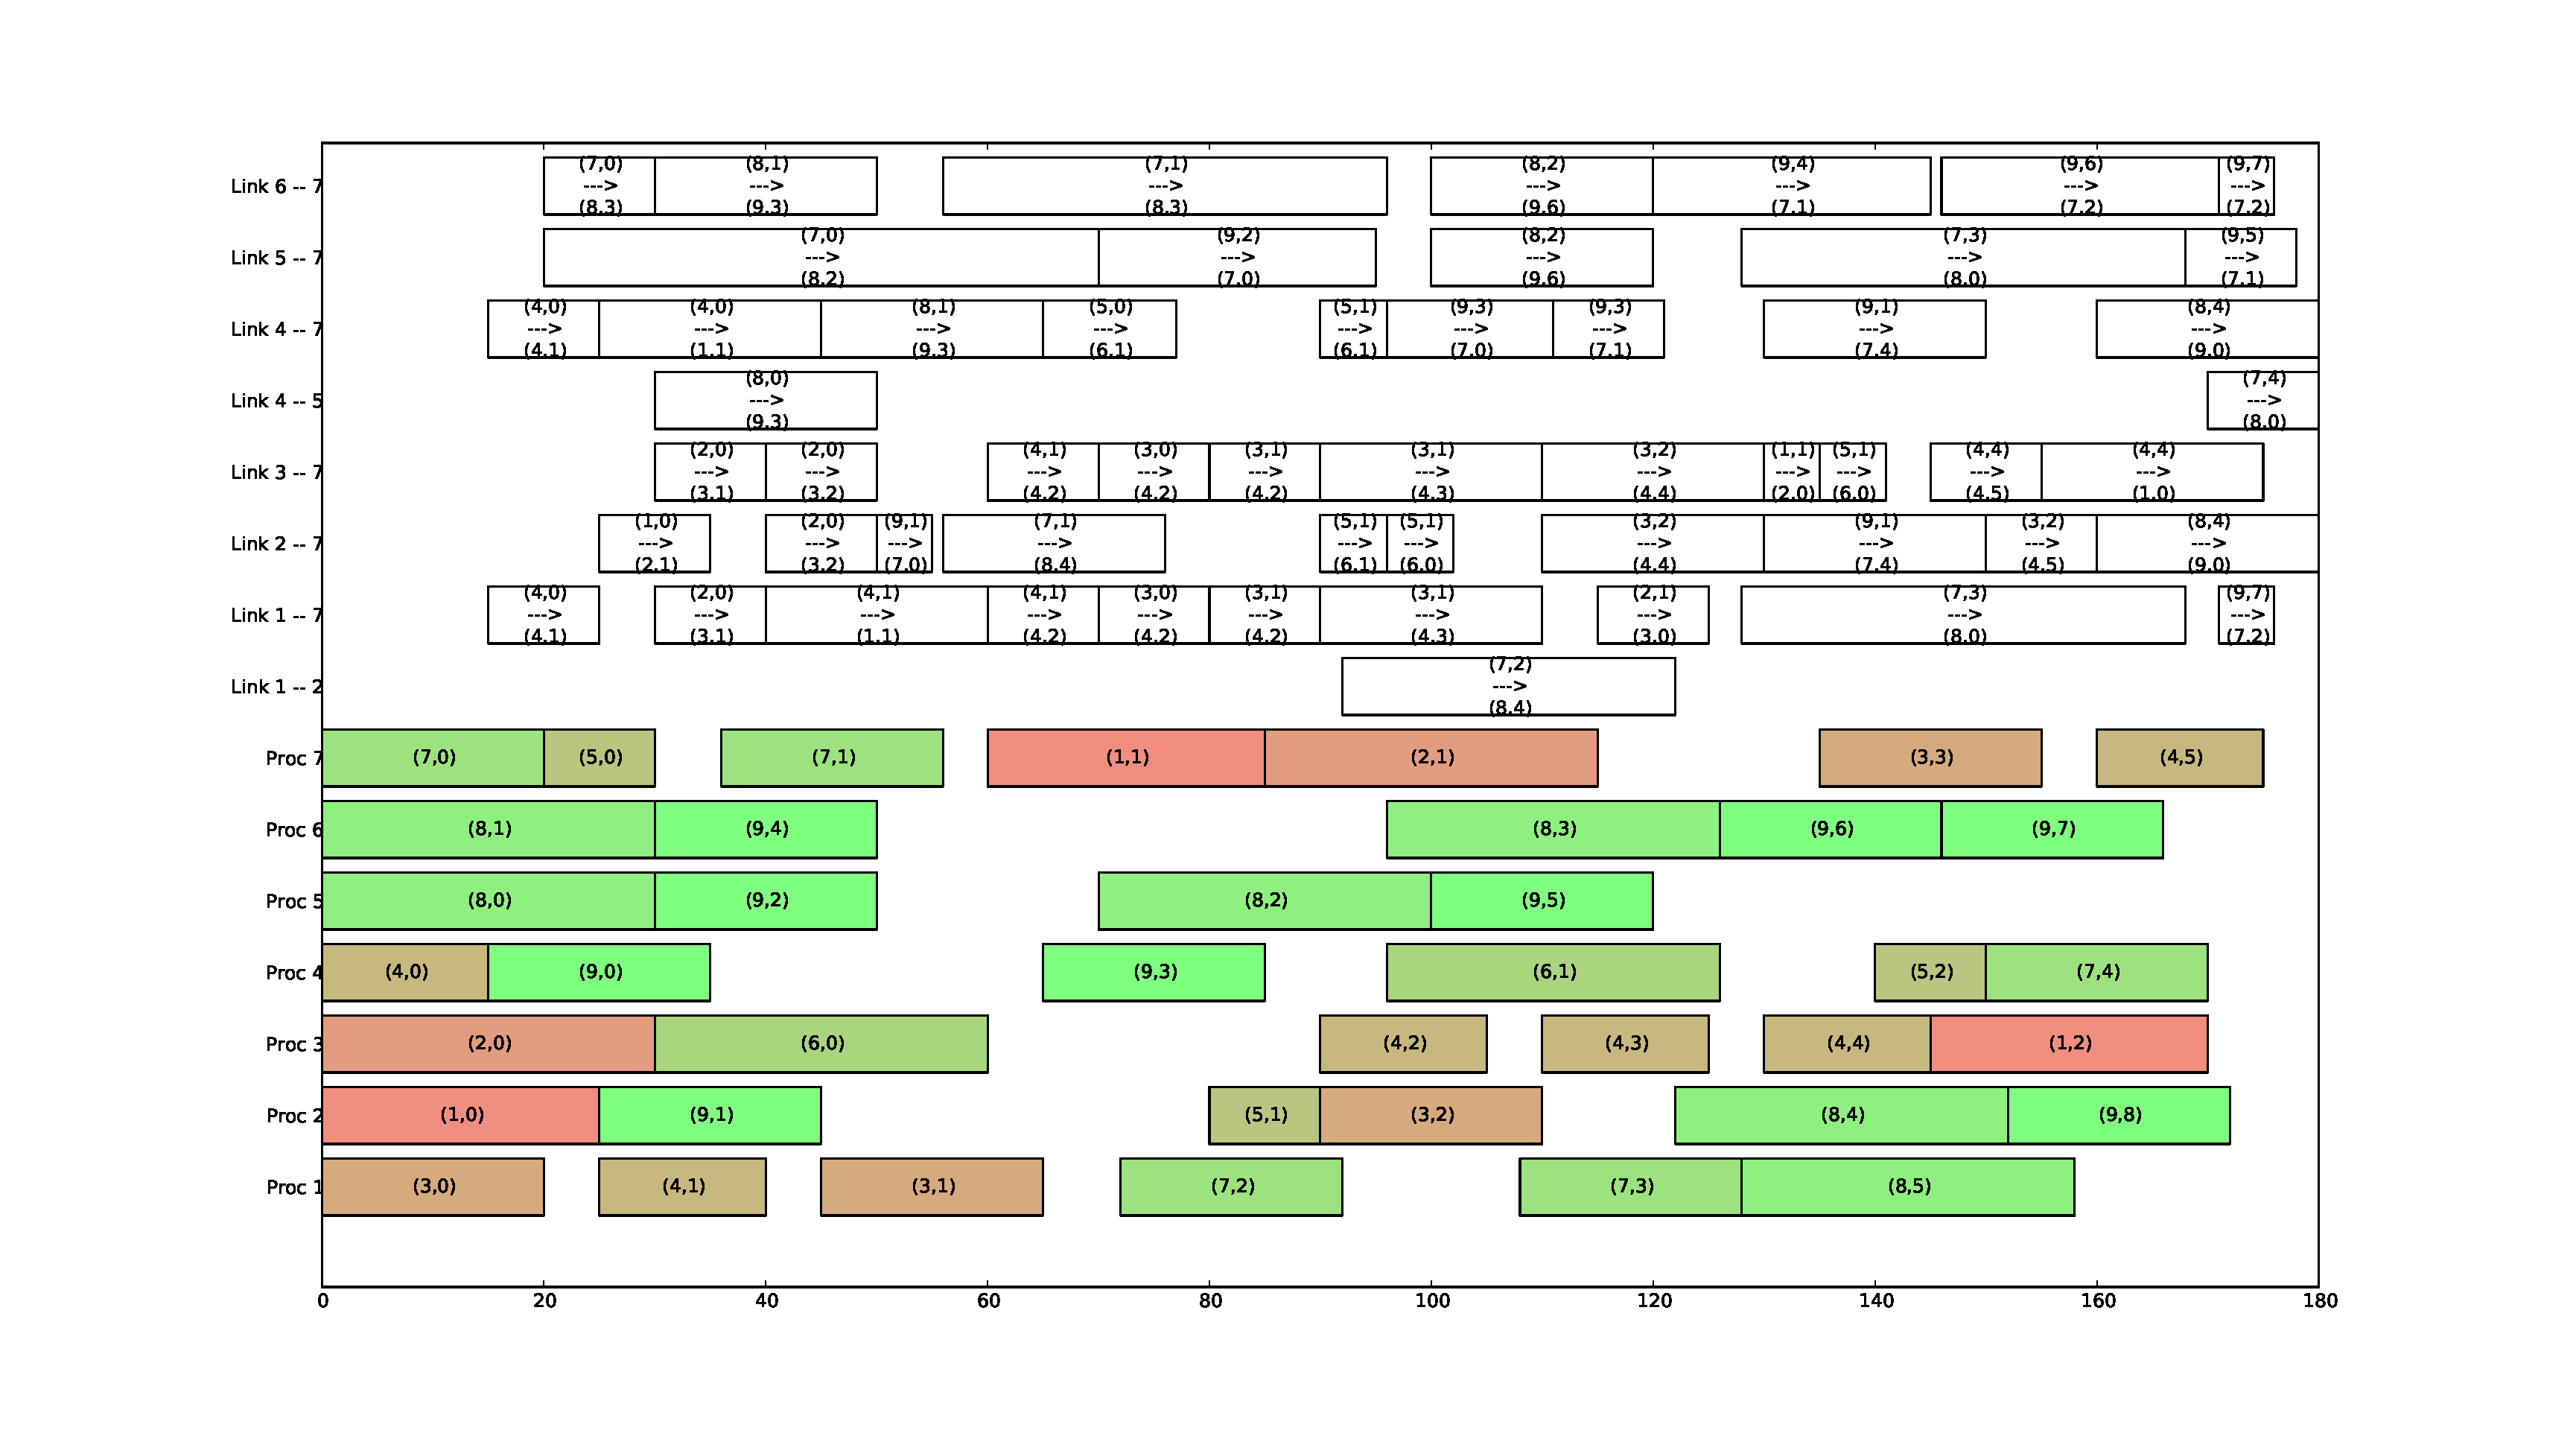
\includegraphics[width=40em]{figure/EXP-9task-sched.pdf}\\
  \caption{9个任务的调度表}\label{EXP-fig-9task}
\end{figure}

如果我们在程序中去除处理器排序部分,使得搜索仅仅按照处理器的序号依次进行。此时,当任务被排在 3 或 4 号结点均可时,未对处理器排序的情况下会将任务排在 3 号处理器上,那么此任务与其他处理器的通信都要经过 7 号处理器,通信较频繁的情况下会造成该链路上消息拥塞,难以调度开。如在上例中,去掉处理器排序后算法模拟程序即无法得到调度结果。

\section{本章小结}

本章首先用例子演示了模拟程序的计算流程,各步的具体结果,并结合最终产生的调度表分析验证了调度结果满足任务的时间及通信约束。本章第二个例子验证了任务的自依赖约束对调度结果产生的影响,最后一个例子验证了处理器排序优化在某些情况下有助于调度过程的搜索。


% 结论与展望
% !Mode:: "TeX:UTF-8"

\chapter*{结论与展望}
\addcontentsline{toc}{chapter}{结论与展望}

\section*{总结论文内容}
本文对包含数据通信而产生数据依赖关系的一组周期性实时任务调度问题提出了针对多核分区系统平台的静态调度算法,解决了任务间同时存在时间约束与数据约束的问题,在进行任务调度的同时,也生成了任务在处理器之间链路上的消息调度。

本文的主要工作内容包括以下几点:

首先,本文针对待解决的调度问题调研了现有的周期性与偶发任务模型和数据驱动的任务模型两类实时任务模型的多核调度算法。分析了现有方法在调度同时包含周期性时间约束和数据通信约束的任务集时的不足之处,并比较了各算法所解决的问题范围以及各自的优劣。

其次,本文在已有算法的基础上设计了面向通信的多核分区静态调度算法,为同时包含通信关系造成的数据依赖以及周期性时间约束任务的调度问题提出了一种解决方案。本文对算法的正确性给出了证明,并提出了处理器排序等优化对调度结果的影响。

最后,本文设计并实现了算法模拟程序,并结合例子验证了算法流程、算法自依赖约束以及处理器排序等因素对调度结果的影响。

\section*{下一步工作展望}

处理跨周期任务及跨周期消息的调度问题,以解决任务时间限大于释放周期的周期性任务的调度,以及某些情况下由于周期内排在后面的任务与下周期任务间消息传递过久,使得消息调度无法在本周期结束,导致的无法调度情况。

研究寻找更好的消息路由方法。最短路有可能造成消息在枢纽节点周围形成拥塞,而不能有效利用外围链路。

虽然由数据依赖造成的优先关系可用SDF描述,但还有一些任务间的优先关系无法用SDF 描述。需要进一步界定用虚拟数据结合SDF可表示的任务间优先关系的集合。

%%%%%%%%%%%%%%%%%%%%%%%%%%%%%%%%%%%%%%%%%%


% Reference
\nocite{*}
\bibliography{subfiles/bibs}
\addcontentsline{toc}{chapter}{参考文献}
\cleardoublepage


% 附录
\appendix
% !Mode:: "TeX:UTF-8"

\chapter{调度程序输入格式}

程序的输入格式如下:

第1行整数 N 表示待调度的总任务数。

接下来 N 行,每行5个整数 C T O D S 分别表示每个任务的最坏执行时间、释放周期、首次释放时间偏移、相对时间限以及任务是否是自依赖的。其中 T 或 D $\leqslant$ 0 则认为该任务非周期任务。

下一行一个整数 K 表示任务间数据通信关系的个数

接下来 K 行,每行5个整数 Tp p Tc c Dpc 分别表示从任务 Tp 产生 p 个数据发送给任务 Tc,每次读入 c 个数据,开始时的 Delay 是 Dpc。

下一行一个整数 J 表示周期倍数因子

下一行一个整数 M 表示目标平台的处理器数

下一行一个整数 s 表示核间通信速率(单位时间传输的数据量)

下一行一个整数 L 表示核间连接数

下面 L 行,每行两个整数 p1 p2 表示处理器 p1 与 p2 相连

%% !Mode:: "TeX:UTF-8"
\chapter{常见问题}
\label{chapter-faq}
\begin{enumerate}
\item 本模板如何使用?
\label{faq-howtouse}
\begin{itemize}
    \item 按照第2章的要求,先下载和安装相应的软件,推荐使用\TeX{}Live2012或更新的版本;
    \item 下载cls文件;
    \item 使用tex的编辑器或其他编辑器,编写论文,注意保存为UTF-8编码;
    \item xelatex编译。
\end{itemize}
注意:\TeX{}Live2012的ISO镜像在\href{http://buaabt.cn/showtopic-214948.aspx}{未来花园BT站}上
有相应的种子可下载,亦可从TUG的\href{http://www.tug.org/texlive/acquire-iso.html}{官方网站}上下载。
\item Windows下的msmake.bat如何使用?
\label{faq-msmake}
\begin{itemize}
    \item 使用Windows的CMD命令行,进入到msmake.bat所在目录;
    \item 键入~msmake~后会显示相应的帮助文件;
    \item 按照所显示的相关信息再键入相应命令即可。
\end{itemize}
注意:由于此批处理文件为编者自行编写,学识有限,代码有许多不如人意之处,
如对此批处理文件有问题可直接邮件联系我(mrpeng000@gmail.com)即可。
\item 使用TexLive如何更新?
\label{faq-texliveupdate}
TUG官方推荐\TeX{}Live通过镜像站进行更新,具体步骤为:
\begin{itemize}
    \item 在“开始”目录下的TeXLive2012文件夹下,找到有TeX Live Manage程序;
    \item 在菜单“tlmgr”下选择“载入其他仓库”,选择最近的仓库即可(如果是北航校内用户并能够
    访问到\href{http://mirror.buaa.edu.cn/}{北航开源镜像站}的话,可以在仓库地址中
    输入\texttt{http://mirror.buaa.edu.cn/CTAN/systems/texlive/tlnet/});
    \item 按照目录选择更新。
\end{itemize}
\end{enumerate}

%% !Mode:: "TeX:UTF-8"
\chapter{联系我们}


% 附页标题样式
\backmatter

% 附页
% !Mode:: "TeX:UTF-8"

\chapter{攻读硕士学位期间取得的学术成果}
%% 此处标题及内容请自行更改
\noindent 发表论文:

\begin{enumerate}
  \item Jinlin Wang. Scheduling of Periodic Tasks with Data Dependency on Multiprocessors[A]. {\em International Conference on Computer Science and Communication Technology}[C], 青岛, 2012. 已录用
\end{enumerate}



%\noindent 发表论文:
%\begin{enumerate}
%
%\item
%Gang Bai and Yue Qi. An Interactive 3D Exhibition System with
% Global Illumination for Digital Museum. In Lecture Notes in
% Computer Science, 2009, Volume 5670, Learning by Playing.
%Game-based Education System Design and Development, Pages 85-92.
%
%\item
%Hu Yong, Qi Yue and Bai Gang. Modeling and Editing Isotropic BRDF.
%In proceedings of the Second International Conference on Modeling,
%Simulation and Visualization Methods (WMSVM). 15-16 May, 2010,
%Sanya, China. Pages 74-77.
%
%\end{enumerate}


%\noindent 申请专利:
%\begin{enumerate}
%
%\item
%齐越,马宗泉,白刚.基于任意位置多球的光源方向标定[P]. 中国发明专利(200910092909), 公开日2010年2 月17 日
%
%\end{enumerate}


\chapter{致谢}

时光荏苒,我的研究生生活即将结束。在这两年多中的时光中,我经历了很多,有过欢笑,有过收获,有过困难,也有过挫折。最重要的是,我从周围的老师、同学、朋友身上学到了很多,有知识方面的积累,也有生活阅历的充实。在此,我要感谢各位老师、同学和家人的关心和帮助。

首先,我要感谢我的导师龙翔教授。龙老师在学科方向上的洞察力和清晰准确的思路让我非常敬佩,与龙老师的讨论使我能够及时发现研究内容的重点,指出我的问题所在,使我收获良多,思路豁然开朗。龙老师严谨治学的态度和对学生悉心关怀使我在学习和生活上都有很大收获。

感谢姜博老师对我的研究内容和论文提出的指导和建议,使我对论文的组织和内容安排有了更清晰的认识。

感谢杨经纬博士在我的研究和准备毕设期间一直对我提供帮助和鼓励,对我研究的内容提出了很多启发性的建议,同时也鞭策我不断努力奋斗。

感谢实验室的所有同学,我们一同生活、一同学习。感谢陈龙、刘乃溪、韩楠、史彪、端文宗,我们一起玩闹、一起吃饭、一起K歌、一起为了共同的目标奋斗,我们互相帮助,使我的研究生生活充实而丰富多彩。

还要感谢家人的养育之恩,感谢他们在我读研期间的关怀和支持,不论遇到任何困难,他们都给我提供最坚实的支持与鼓励,让我能够向着自己的目标不断前进。


\end{document}
